% appendix/whymb/whymemorybarriers.tex

\QuickQuizChapter{chp:app:whymb:Why Memory Barriers?}{Why Memory Barriers?}

그래서 무엇이 CPU 설계자들을 불쌍하고 의심할 줄 모르는 SMP 소프트웨어
설계자들에게 메모리 배리어를 주게 만들었을까요?

한마디로, 메모리 참조 순서 재배치는 성능을 훨씬 좋게 만들고, 따라서 올바른 동작
여부가 메모리 참조 순서에 의존적인 동기화와 같은 작업에는 순서를 강제하기 위해
메모리 배리어가 필요해졌습니다.
\iffalse

So what possessed CPU designers to cause them to inflict memory barriers
on poor unsuspecting SMP software designers?

In short, because reordering memory references allows much better performance,
and so memory barriers are needed to force ordering in things like
synchronization primitives whose correct operation depends on ordered
memory references.
\fi

이 질문에 더 자세한 답변을 얻기 위해선 어떻게 CPU 캐시들이 동작하는지, 특히
캐시가 정말 잘 동작하게 하기 위해 필요한게 무엇인지에 대한 깊은 이해가
필요합니다.
다음의 섹션들은:
\begin{enumerate}
\item	캐시의 구조를 보이고,
\item	캐시 일관성 프로토콜이 어떻게 CPU 들이 메모리의 각 위치의 값들에 대해
	합의하며, 마지막으로,
\item	어떻게 스토어 버퍼들과 인밸리데이트 큐들이 캐시와 캐시 일관성
	프로토콜이 높은 성능을 얻을 수 있게 돕는지 알아봅니다.
\end{enumerate}
우린 메모리 배리어들이 좋은 성능과 확장성을 위한 필요악이고, CPU 들이 그들
사이의 접합부보다도, 그들이 접근하려 시도하는 메모리 보다도 훨씬 빠르다는
사실로부터 기인했음을 보게 될 것입니다.
\iffalse

Getting a more detailed answer to this question requires a good understanding
of how CPU caches work, and especially what is required to make
caches really work well.
The following sections:
\begin{enumerate}
\item	present the structure of a cache,
\item	describe how cache-coherency protocols ensure that CPUs agree
	on the value of each location in memory, and, finally,
\item	outline how store buffers and invalidate queues help
	caches and cache-coherency protocols achieve high performance.
\end{enumerate}
We will see that memory barriers are a necessary evil that is required
to enable good performance and scalability, an evil that stems from
the fact that CPUs are orders of magnitude faster than are both the
interconnects between them and the memory they are attempting to access.
\fi

\section{Cache Structure}
\label{sec:app:whymb:Cache Structure}

현대의 CPU 들은 현대의 메모리 시스템들보다 훨씬 빠릅니다.
2006 년의 CPU 는 나노세컨드당 열개의 인스트럭션들을 수행할 수 있습니다만, 메인
메모리에서 데이터 아이템 하나를 가져오는데엔 수십 나노세컨드를 필요로 할겁니다.
이 속도의 간극 --- 100 배가 넘는 --- 이 현대 CPU 에서 볼 수 있는 수
메가바이트의 캐시를 있게 했습니다.
이런 캐시들은 Figure~\ref{fig:app:whymb:Modern Computer System Cache Structure}
에 보여졌듯, CPU 들과 연관되어지고 수 사이클만에 접근될 수 있습니다.\footnote{
	CPU 에 가깝게 작고 한 사이클의 액세스 타임을 갖는 1단계 캐시를, 그
	다음엔 더 크고, 약 10 사이클 정도의 긴 액세스 타임을 갖는 2단계 캐시를
	두는 식으로 여러 단계의 캐시를 사용하는건 표준적인 일입니다.
	고성능 CPU 는 종종 세단계 또는 네단계까지도 캐시를 둡니다.}
\iffalse

Modern CPUs are much faster than are modern memory systems.
A 2006 CPU might be capable of executing ten instructions per nanosecond,
but will require many tens of nanoseconds to fetch a data item from
main memory.
This disparity in speed --- more than two orders of magnitude --- has
resulted in the multi-megabyte caches found on modern CPUs.
These caches are associated with the CPUs as shown in
Figure~\ref{fig:app:whymb:Modern Computer System Cache Structure},
and can typically be accessed in a few cycles.\footnote{
	It is standard practice to use multiple levels of cache,
	with a small level-one cache close to the CPU with
	single-cycle access time, and a larger level-two cache
	with a longer access time, perhaps roughly ten clock cycles.
	Higher-performance CPUs often have three or even four levels
	of cache.}
\fi

\begin{figure}[htb]
\begin{center}
\resizebox{3in}{!}{\includegraphics{appendix/whymb/cacheSC}}
\end{center}
\caption{Modern Computer System Cache Structure}
\label{fig:app:whymb:Modern Computer System Cache Structure}
\end{figure}

CPU 의 캐시와 메모리 사이의 데이터 흐름은 ``캐시 라인'' 이라 불리는, 일반적으로
16 과 256 사이의 2의 거듭제곱 바이트 크기인, 고정된 길이의 블록 단위로
이루어집니다.
한 데이터 아이템이 한 CPU 에 의해 처음 액세스 되면, 그 아이템은 해당 CPU 의
캐시에 없을 것이고, 이는 곧 ``캐시 미스'' (또는, 보다 분명히 말하면,
``스타트업'' 또는 ``웜업'' 캐시 미스) 를 의미합니다.
이 캐시 미스는 CPU 는 해당 아이템이 메모리로부터 얻어져 오는 동안 수백 사이클을
기다려야 (또는 ``스톨'' 되어야) 함을 의미합니다.
하지만, 해당 아이템은 해당 CPU 의 캐시 위에 로드될 것이고, 따라서 다음의 액세스는
해당 아이템을 캐시에서 찾아낼 것이고, 따라서 최대 속도로 처리될 것입니다.
\iffalse

Data flows among the CPUs' caches and memory in fixed-length blocks
called ``cache lines'', which are normally a power of two in size,
ranging from 16 to 256 bytes.
When a given data item is first accessed by a given CPU, it will
be absent from that CPU's cache, meaning that a ``cache miss''
(or, more specifically, a ``startup'' or ``warmup'' cache miss)
has occurred.
The cache miss means that the CPU will
have to wait (or be ``stalled'') for hundreds of cycles while the
item is fetched from memory.
However, the item will be loaded into that CPU's cache, so that
subsequent accesses will find it in the cache and therefore run
at full speed.
\fi

시간이 지난 후, 이 CPU 의 캐시는 꽉 찰 것이고, 이후의 미스들은 새로 가져온
아이템들을 위한 공간을 만들기 위해 캐시로부터 아이템을 비울 것을 필요로 할 수
있습니다.
그런 캐시 미스는 캐시의 제한된 용량으로 인해 발생하기 때문에 ``용량 미스'' 라고
불리웁니다.
하지만, 대부분의 캐시들은 아직 용량이 꽉 차지 않았다 해도 새 아이템의 공간을
만들기 위해 오래된 아이템을 비우도록 강제되기도 합니다.
이는 커다란 캐시들은 Figure~\ref{fig:app:whymb:CPU Cache Structure} 체이닝 없이
고정된 크기의 해시 버켓 (CPU 설계자들이 부르는 용어로는 ``set'') 들을 사용하는
하드웨어 해시 테이블로 구현되어 있기 때문입니다.
\iffalse

After some time, the CPU's cache will fill, and subsequent
misses will likely need to eject an item from the cache in order
to make room for the newly fetched item.
Such a cache miss is termed a ``capacity miss'', because it is caused
by the cache's limited capacity.
However, most caches can be forced to eject an old item to make room
for a new item even when they are not yet full.
This is due to the fact that large caches are implemented as hardware
hash tables with fixed-size hash buckets (or ``sets'', as CPU designers
call them) and no chaining, as shown in
Figure~\ref{fig:app:whymb:CPU Cache Structure}.
\fi

이 캐시는 16개의 ``set'' 들과 두개의 ``way'' 를 가져서 총 32개의 ``라인'' 을
가지며, 각 엔트리는 256 바이트의 ``캐시 라인'' 하나를 담는, 256 바이트 정렬
블록의 메모리입니다.
이 캐시 라인 크기는 좀 작지만, 16진수 계산을 훨씬 간단하게 해줄 겁니다.
하드웨어 용어로, 이것은 two-way set-associative 캐시 라고 불리우며, 16개의
버켓을 가지고, 각 버켓은 최대 두개의 원소를 가질 수 있는 해시 체인인 소프트웨어
해시 테이블로 비유될 수 있습니다.
사이즈 (이 경우 32 개의 캐시 라인들) 와 associativity (이 경우 2) 는 함께
캐시의 ``기하 도형적 배열 (geometry)'' 이라 불립니다.
이 캐시는 하드웨어로 구현되었기 때문에, 해시 함수는 엄청 간단합니다: 메모리
어드레스에서 네개의 비트를 뽑아냅니다.
\iffalse

This cache has sixteen ``sets'' and two ``ways'' for a total of 32
``lines'', each entry containing a single 256-byte ``cache line'',
which is a 256-byte-aligned block of memory.
This cache line size is a little on the large size, but makes the hexadecimal
arithmetic much simpler.
In hardware parlance, this is a two-way set-associative cache, and
is analogous to a software hash table with
sixteen buckets, where each bucket's hash chain is limited to
at most two elements.
The size (32 cache lines in this case) and the associativity (two in
this case) are collectively called the cache's ``geometry''.
Since this cache is implemented in hardware, the hash function is
extremely simple: extract four bits from the memory address.
\fi

\begin{figure}[t]
\begin{center}
\small
\begin{picture}(170,170)(0,0)

	% Addresses

	\put(0,0){\makebox(20,10){\tt 0xF}}
	\put(0,10){\makebox(20,10){\tt 0xE}}
	\put(0,20){\makebox(20,10){\tt 0xD}}
	\put(0,30){\makebox(20,10){\tt 0xC}}
	\put(0,40){\makebox(20,10){\tt 0xB}}
	\put(0,50){\makebox(20,10){\tt 0xA}}
	\put(0,60){\makebox(20,10){\tt 0x9}}
	\put(0,70){\makebox(20,10){\tt 0x8}}
	\put(0,80){\makebox(20,10){\tt 0x7}}
	\put(0,90){\makebox(20,10){\tt 0x6}}
	\put(0,100){\makebox(20,10){\tt 0x5}}
	\put(0,110){\makebox(20,10){\tt 0x4}}
	\put(0,120){\makebox(20,10){\tt 0x3}}
	\put(0,130){\makebox(20,10){\tt 0x2}}
	\put(0,140){\makebox(20,10){\tt 0x1}}
	\put(0,150){\makebox(20,10){\tt 0x0}}

	% Way 0

	\put(20,163){\makebox(80,10){Way 0}}
	\put(20,0){\framebox(80,10){\tt }}
	\put(20,10){\framebox(80,10){\tt 0x12345E00}}
	\put(20,20){\framebox(80,10){\tt 0x12345D00}}
	\put(20,30){\framebox(80,10){\tt 0x12345C00}}
	\put(20,40){\framebox(80,10){\tt 0x12345B00}}
	\put(20,50){\framebox(80,10){\tt 0x12345A00}}
	\put(20,60){\framebox(80,10){\tt 0x12345900}}
	\put(20,70){\framebox(80,10){\tt 0x12345800}}
	\put(20,80){\framebox(80,10){\tt 0x12345700}}
	\put(20,90){\framebox(80,10){\tt 0x12345600}}
	\put(20,100){\framebox(80,10){\tt 0x12345500}}
	\put(20,110){\framebox(80,10){\tt 0x12345400}}
	\put(20,120){\framebox(80,10){\tt 0x12345300}}
	\put(20,130){\framebox(80,10){\tt 0x12345200}}
	\put(20,140){\framebox(80,10){\tt 0x12345100}}
	\put(20,150){\framebox(80,10){\tt 0x12345000}}

	% Way 1

	\put(100,163){\makebox(80,10){Way 1}}
	\put(100,0){\framebox(80,10){\tt }}
	\put(100,10){\framebox(80,10){\tt 0x43210E00}}
	\put(100,20){\framebox(80,10){\tt }}
	\put(100,30){\framebox(80,10){\tt }}
	\put(100,40){\framebox(80,10){\tt }}
	\put(100,50){\framebox(80,10){\tt }}
	\put(100,60){\framebox(80,10){\tt }}
	\put(100,70){\framebox(80,10){\tt }}
	\put(100,80){\framebox(80,10){\tt }}
	\put(100,90){\framebox(80,10){\tt }}
	\put(100,100){\framebox(80,10){\tt }}
	\put(100,110){\framebox(80,10){\tt }}
	\put(100,120){\framebox(80,10){\tt }}
	\put(100,130){\framebox(80,10){\tt }}
	\put(100,140){\framebox(80,10){\tt }}
	\put(100,150){\framebox(80,10){\tt }}

\end{picture}
\end{center}
\caption{CPU Cache Structure}
\label{fig:app:whymb:CPU Cache Structure}
\end{figure}

Figure~\ref{fig:app:whymb:CPU Cache Structure} 에서 각 박스는 256 바이트 캐시
라인을 담는 캐시 엔트리를 나타냅니다.
하지만, 캐시 엔트리는 그림의 빈 박스처럼 비어있을 수도 있습니다.
그 외의 박스들은 각 엔트리가 담고 있는 캐시 라인의 메모리 주소들을 표시하고
있습니다.
캐시 라인들은 256 바이트로 정렬되어야 하기 때문에, 각 주소의 하위 8 비트는
0입니다, 그리고 하드웨어 해시 함수는 그 다음 4개 상위 비트를 해시 라인 넘버로
매치시킵니다.
\iffalse

In Figure~\ref{fig:app:whymb:CPU Cache Structure},
each box corresponds to a cache entry, which
can contain a 256-byte cache line.
However, a cache entry can be empty, as indicated by the empty boxes
in the figure.
The rest of the boxes are flagged with the memory address of the cache line
that they contain.
Since the cache lines must be 256-byte aligned, the low eight bits of
each address are
zero, and the choice of hardware hash function means that the next-higher
four bits match the hash line number.
\fi

그림에 그려진 상황은 프로그램의 코드가 메모리 주소로 0x43210E00 부터 0x43210EFF
사이에 위치하고, 이 프로그램이 0x12345000 부터 0x12345EFF 까지의 데이터를
순차적으로 접근했다면 나타날 것입니다.
이 프로그램이 이제 0x12345F00 을 접근하려 한다고 생각해 봅시다.
이 위치는 0xF 열로 해시되고, 이 라인의 두 way 는 모두 비어있으므로, 이로 인한
256 바이트 라인은 캐시에 들어올 수 있습니다.
만약 프로그램이 0x1233000 위치를 액세스 하려 한다면, 0x0 열로 해시되고, 이로
인한 256 바이트 캐시 라인은 way 1 에 들어올 수 있습니다.
하지만, 만약 프로그램이 0x1233E00 위치에 액세스 한다면, 0xE 열로 해시되는데,
여기 존재하는 것들 중 하나는 새로 들어올 캐시 라인을 위한 공간을 만들기 위해
비워져야 합니다.
만약 이렇게 비워진 캐시 라인이 나중에 액세스 된다면, 캐시 미스가 날겁니다.
그러한 캐시 미스를 ``associativity miss'' 라고 합니다.
\iffalse

The situation depicted in the figure might arise if the program's code
were located at address 0x43210E00 through 0x43210EFF, and this program
accessed data sequentially from 0x12345000 through 0x12345EFF.
Suppose that the program were now to access location 0x12345F00.
This location hashes to line 0xF, and both ways of this line are
empty, so the corresponding 256-byte line can be accommodated.
If the program were to access location 0x1233000, which hashes to line
0x0, the corresponding 256-byte cache line can be accommodated in
way 1.
However, if the program were to access location 0x1233E00, which hashes
to line 0xE, one of the existing lines must be ejected from the cache
to make room for the new cache line.
If this ejected line were accessed later, a cache miss would result.
Such a cache miss is termed an ``associativity miss''.
\fi

지금까지는 CPU 가 데이터 아이템을 읽는 경우만 생각해봤습니다.
쓰기를 하면 어떻게 될까요?
주어진 데이터 아이템의 값에 대해 모든 CPU 가 동의를 하는 것이 중요하기에, CPU
는 어떤 데이터 아이템에 값을 쓰기 전에, 먼저 그 아이템을 다른 CPU 의 캐시에서
삭제하거나, ``무효화 (invalidate)'' 시켜야만 합니다.
무효화 작업이 완료되면, 이 CPU 는 안전하게 해당 데이터 아이템을 수정할 수
있습니다.
만약 해당 데이터 아이템이 이 CPU 의 캐시에 존재했다면, 그러나 읽기
전용이었다면, 이 작업은 ``write miss'' 라고 합니다.
CPU 가 주어진 데이터 아이템을 다른 CPU 의 캐시들로부터 무효화 시키는데
성공하면, 이 CPU 는 해당 데이터 아이템을 반복적으로 쓸 수 (그리고 읽을수도)
있습니다.
\iffalse

Thus far, we have been considering only cases where a CPU reads
a data item.
What happens when it does a write?
Because it is important that all CPUs agree on the value of a given
data item, before a given CPU writes to that data item, it must first
cause it to be removed, or ``invalidated'', from other CPUs' caches.
Once this invalidation has completed, the CPU may safely modify the
data item.
If the data item was present in this CPU's cache, but was read-only,
this process is termed a ``write miss''.
Once a given CPU has completed invalidating a given data item from other
CPUs' caches, that CPU may repeatedly write (and read) that data item.
\fi

나중에, 다른 CPU 가 해당 데이터 아이템에 접근하려 하면, 이번엔 첫번째 CPU 가 그
아이템에 쓰기를 하려고 그 아이템을 무효화 시켰기 때문에 캐시 미스가 납니다.
이런 캐시 미스는 일반적으로 일부 CPU 들이 데이터 아이템을 커뮤니케이션에
사용하려 해서 (예를 들어, 락은 CPU 들 사이에서 상호 배제적 알고리즘을 위한
커뮤니케이션에 사용되는 데이터 아이템입니다) 발생하기 때문에, ``커뮤니케이션
미스'' 라고 합니다.

분명히, 모든 CPU 들이 해당 데이터에 일관된 시야를 유지하도록 보장하는데 많은
주의를 기울여야만 합니다.
이 데이터 가져오기, 무효화 하기, 쓰기 작업을 통해, 데이터를 잃어버리거나 (더
나쁘게도) 다른 CPU 들이 같은 데이터 아이템에 대해 각자의 캐시에 다른 값을 갖게
되는 경우를 상상해 볼 수 있습니다.
이런 문제는 다음 섹션에서 다루는 ``캐시 일관성 프로토콜'' 에 의해 방지됩니다.
\iffalse

Later, if one of the other CPUs attempts to access the data item, it
will incur a cache miss, this time because the first CPU invalidated
the item in order to write to it.
This type of cache miss is termed a ``communication miss'', since it
is usually due to several CPUs using the data items to communicate
(for example, a lock is a data item that is used to communicate among
CPUs using a mutual-exclusion algorithm).

Clearly, much care must be taken to ensure that all CPUs maintain
a coherent view of the data.
With all this fetching, invalidating, and writing, it is easy to
imagine data being lost or (perhaps worse) different CPUs having
conflicting values for the same data item in their respective
caches.
These problems are prevented by ``cache-coherency protocols'',
described in the next section.
\fi

\section{Cache-Coherence Protocols}
\label{sec:app:whymb:Cache-Coherence Protocols}

캐시 일관성 프로토콜은 비일관적인 상황이나 데이터 유실을 막기 위해 캐시 라인
상태를 관리합니다.
이런 프로토콜은 열개 이상의 상태를 가져서 매우 복잡할 수 있습니다만, \footnote{
	SGI Origin2000 의 9개 상태, Sequent (이제는 IBM) NUMA-Q 의 26개 상태
	그림을 보기 위해 Culler et al.~\cite{DavidECuller1999} 670 페이지와 671
	페이지를 참고하세요.
	두 그림 모두 실제보다는 단순합니다.}
우리의 목적을 위해서는 MESI 캐시 일관성 프로토콜의 네가지 상태에 대해서만
신경쓰면 됩니다.
\iffalse

Cache-coherency protocols manage cache-line states so as to prevent
inconsistent or lost data.
These protocols can be quite complex, with many tens
of states,\footnote{
	See Culler et al.~\cite{DavidECuller1999} pages 670 and 671
	for the nine-state and 26-state diagrams for SGI Origin2000
	and Sequent (now IBM) NUMA-Q, respectively.
	Both diagrams are significantly simpler than real life.}
but for our purposes we need only concern ourselves with the
four-state MESI cache-coherence protocol.
\fi

\subsection{MESI States}
\label{sec:app:whymb:MESI States}

MESI 는 한 캐시 라인이 이 프로토콜을 통해 가질 수 있는 네가지 상태인
``modified'', ``exclusive'', ``shared'', 그리고 ``invalid'' 의 약자입니다.
따라서 이 프로토콜을 사용하는 캐시는 캐시라인마다 해당 라인의 물리 주소와
데이터 이외에도 두 비트의 상태 ``tag'' 를 갖습니다.

``modified'' 상태의 라인은 연관된 CPU 가 최근에 메모리 스토어를 했고, 연관된
메모리는 다른 CPU 의 캐시에 존재하지 않음이 보장됩니다.
따라서 ``modified'' 상태의 캐시 라인들은 해당 CPU 에 의해 ``소유된 상태''
라고도 이야기 합니다.
이 캐시는 최신 상태의 데이터 카피만을 가지고 있으므로, 이 캐시는 메모리의 예전
데이터를 최신 데이터로 갱신하거나 다른 캐시에게 넘기거나 할 의무를 가지고
있으며, 그 의무는 이 라인이 다른 데이터를 가지게 되기 전에 반드시 수행되어야만
합니다.
\iffalse

MESI stands for ``modified'', ``exclusive'', ``shared'', and ``invalid'',
the four states a given cache line can take on using this
protocol.
Caches using this protocol therefore maintain a two-bit state ``tag'' on each
cache line in addition to that line's physical address and data.
% cite Schimmel's book on virtual caches.

A line in the ``modified'' state has been subject to a recent memory store
from the corresponding CPU, and the corresponding memory is guaranteed
not to appear in any other CPU's cache.
Cache lines in the ``modified'' state can thus be said to be ``owned''
by the CPU.
Because this cache holds the only up-to-date copy of the data, this
cache is ultimately responsible for either writing it back to memory
or handing it off to some other cache, and must do so before reusing
this line to hold other data.
\fi

``exclusive'' 상태는 ``modified'' 상태와 유사합니다만, 해당 캐시 라인은 연관된
CPU 에 의해 수정되지 않은 상태라는 점이 유일한 차이점으로, 메모리에 있는 캐시
라인의 데이터의 복사본이 최신 버전이란 뜻입니다.
하지만, CPU 는 다른 CPU 의 눈치를 보지 않고 언제든 이 라인에 언제든 스토어를 할
수 있으므로, ``exclusive'' 상태의 라인은 연관된 CPU 에 소유되어 있다고 이야기
할 수 있습니다.
그렇다곤 하나, 메모리에 있는 값이 최신 상태이므로, 이 캐시는 데이터를 메모리에
다시 돌려넣거나 다른 CPU 에게 넘기지 않고 버릴 수 있습니다.
\iffalse

The ``exclusive'' state is very similar to the ``modified'' state,
the single exception being that the cache line has not yet been
modified by the corresponding CPU, which in turn means that the
copy of the cache line's data that resides in memory is up-to-date.
However, since the CPU can store to this line at any time, without
consulting other CPUs, a line in the ``exclusive'' state can still
be said to be owned by the corresponding CPU.
That said, because the corresponding value in memory is up to date,
this cache can discard this data without writing it back to memory
or handing it off to some other CPU.
\fi

``shared'' 상태의 라인은 적어도 한개의 다른 CPU 의 캐시에는 복사되어 있으며,
따라서 이 PU 는 먼저 다른 CPU 에게 이야기를 하지 않고서는 해당 라인에 스토어를
할 수 없습니다.
``exclusive'' 상태처럼, 메모리에 있는 값은 최신 버전이므로, 이 캐시는 메모리에
값을 다시 돌려놓거나 다른 CPU 에게 넘기지 않고 그 데이터를 버릴 수 있습니다.
\iffalse

A line in the ``shared'' state might be replicated in at least
one other CPU's cache, so that this CPU is not permitted to store
to the line without first consulting with other CPUs.
As with the ``exclusive'' state, because the corresponding value
in memory is up to date,
this cache can discard this data without writing it back to memory
or handing it off to some other CPU.
\fi

``invalide'' 상태의 라인은 비어있는데, 달리 말하자면, 아무 값도 들고 있지
않습니다.
새로운 데이터는 캐시에 들어올 때, 가능하다면 ``invalid'' 상태의 캐시 라인에
위치합니다.
다른 상태에 있는 라인을 교체하는 것은 교체된 라인이 미래에 다시 참조될 때 비싼
캐시 미스가 발생할 수 있기 때문에 이런 방법이 선호됩니다.

캐시 라인의 데이터에 대해 모든 CPU 가 일관적인 뷰를 유지해야 하기 때문에, 이
캐시 일관성 프로토콜은 시스템 사이의 캐시 라인의 이동을 조정하기 위해 메세지를
제공합니다.
\iffalse

A line in the ``invalid'' state is empty, in other words, it holds
no data.
When new data enters the cache, it is placed into a
cache line that was in the ``invalid'' state if possible.
This approach is preferred because replacing a line in any other
state could result in an expensive cache miss should the replaced
line be referenced in the future.

Since all CPUs must maintain a coherent view of the data carried in
the cache lines, the cache-coherence protocol provides messages
that coordinate the movement of cache lines through the system.
\fi

\subsection{MESI Protocol Messages}
\label{sec:app:whymb:MESI Protocol Messages}

앞 섹션에서 이야기한 많은 작업들은 CPU 간의 통신을 필요로 합니다.
만약 CPU 들이 하나의 공유된 버스만을 사용한다면, 다음과 같은 메세지들 만으로도
충분합니다:
\iffalse

Many of the transitions described in the previous section require
communication among the CPUs.
If the CPUs are on a single shared bus, the following messages suffice:
\fi
\begin{itemize}
\item	Read:
	``Read'' 메세지는 읽혀질 캐시 라인의 물리 주소를 담습니다.
\item	Read Response:
	``Read response'' 메세지는 앞의 ``read'' 메세지에서 요청받은 데이터를
	담습니다.
	이 ``read response'' 메세지는 메모리에서 또는 캐시들 중 하나에서
	얻어와질 수도 있습니다.
	예를 들어, 캐시들 가운데 하나가 현재 필요로 하는 데이터를 ``modified''
	상태로 가지고 있다면, 그 캐시가 ``read response'' 메세지를 보내야
	합니다.
\item	Invalidate:
	``Invalidate'' 메세지는 무효화할 캐시 라인의 물리 주소를 담습니다.
	모든 다른 캐시들은 그 데이터를 각자의 캐시에서 제거하고 답장을 해야
	합니다.
\item	Invalidate Acknowledge:
	``Invalidate'' 메세지를 받은 CPU 는 반드시 요청된 데이터를 자신의 CPU
	로부터 제거한 후 ``nvalidate acknowledge'' 메세지를 보내야 합니다.
\iffalse

\item	Read:
	The ``read'' message contains the physical address of the cache line
	to be read.
\item	Read Response:
	The ``read response'' message contains the data requested by an
	earlier ``read'' message.
	This ``read response'' message might be supplied either by
	memory or by one of the other caches.
	For example, if one of the caches has the desired data in
	``modified'' state, that cache must supply the ``read response''
	message.
\item	Invalidate:
	The ``invalidate'' message contains the physical address of the
	cache line to be invalidated.
	All other caches must remove the corresponding data from their
	caches and respond.
\item	Invalidate Acknowledge:
	A CPU receiving an ``invalidate'' message must respond with an
	``invalidate acknowledge'' message after removing the specified
	data from its cache.
\fi
\item	Read Invalidate:
	``Read Invalidate'' 메세지는 읽음과 동시에 다른 캐시들로부터는 제거할
	캐시 라인의 물리 주소를 담습니다.
	따라서, 이름으로부터 알 수 있듯 이것은 ``read'' 와 ``invalidate'' 의
	조합인 셈입니다.
	``read invalidate'' 메세지는 ``read response'' 와 ``invalidate
	acknowledge'' 메세지 둘 다 응답으로 받습니다.
\item	Writeback:
	``writeback'' 메세지는 메모리에 도로 쓰여질  (그리고 그 과정에서 다른
	CPU 의 캐시에 ``snooped'' 를 보낼 수 있을 겁니다) 데이터와 주소를 모두
	담습니다.
	이 메세지는 캐시들이 ``modified'' 상태의 라인을 다른 데이터를 위한
	공간을 만들어야 하거나 할 때 제거할 수 있도록 합니다.
\iffalse

\item	Read Invalidate:
	The ``read invalidate'' message contains the physical address
	of the cache line to be read, while at the same time directing
	other caches to remove the data.
	Hence, it is a combination of a ``read'' and an ``invalidate'',
	as indicated by its name.
	A ``read invalidate'' message requires both a ``read response''
	and a set of ``invalidate acknowledge'' messages in reply.
\item	Writeback:
	The ``writeback'' message contains both the address and the
	data to be written back to memory (and perhaps ``snooped''
	into other CPUs' caches along the way).
	This message permits caches to eject lines in the ``modified''
	state as needed to make room for other data.
\fi
\end{itemize}

\QuickQuiz{}
	Writeback 메세지는 어디서 와서 어디로 가나요?
	\iffalse
	Where does a writeback message originate from and where does
	it go to?
	\fi
\QuickQuizAnswer{
	Writeback 메세지는 해당 CPU 에서, 또는 일부 설계에서는 해당 CPU 의
	캐시의 해당 레벨에서 발생합니다---또는 심지어 여러 CPU 들 사이에 공유된
	캐시에서도.
	핵심은 해당 캐시는 현재 데이터 아이템을 위한 공간이 없어서 공간을
	만들기 위해 캐시에서 일부 데이터를 제거해야 한다는 겁니다.
	다른 캐시나 메모리에 데이터의 복사본이 일부 존재한다면, 그 부분은
	writeback 메세지 필요 없이 그냥 버려질 수도 있습니다.

	반면, 만약 제거될 데이터의 모든 부분이 수정된 상태여서 최신 버전이 이
	캐시에만 존재한다면, 그런 데이터 아이템들은 어딘가 다른곳에
	복사되어야만 합니다.
	이 복사 과정이 ``writeback 메세지'' 를 통해 이루어집니다.
	\iffalse

	The writeback message originates from a given CPU, or in some
	designs from a given level of a given CPU's cache---or even
	from a cache that might be shared among several CPUs.
	The key point is that a given cache does not have room for
	a given data item, so some other piece of data must be ejected
	from the cache to make room.
	If there is some other piece of data that is duplicated in some
	other cache or in memory, then that piece of data may be simply
	discarded, with no writeback message required.

	On the other hand, if every piece of data that might be ejected
	has been modified so that the only up-to-date copy is in this
	cache, then one of those data items must be copied somewhere
	else.
	This copy operation is undertaken using a ``writeback message''.
	\fi

	Writeback 메세지의 목적지는 새 값을 쓸 수 있는 곳이어야 합니다.
	이는 메인 메모리가 될 수도 있지만, 다른 캐시일 수도 있습니다.
	만약 그게 캐시라면, 그 캐시는 보통 같은 CPU 의 높은 레벨 캐시로, 예를
	들어, 레벨-1 캐시는 레벨-2 캐시에 writeback 을 할 수도 있습니다.
	하지만, 일부 하드웨어 설계는 CPU 간 writeback 을 허용해서, CPU~0 의
	캐시는 CPU~1 에 writeback 메세지를 날릴 수 있ㅅ브니다.
	이는 보통 CPU~1 이 어떻게든, 예를 들어, 최근에 읽기 리퀘스트를
	했다던지와 같이 그 데이터에 흥미를 표했다면 행해질 수 있습니다.

	한마디로, writeback 메세지는 공간이 부족한 시스템의 어떤 부분에서
	보내질 수 있고, 그 데이터를 수용할 수 있는 시스템의 다른 부분에서 받게
	됩니다.
	\iffalse

	The destination of the writeback message has to be something
	that is able to store the new value.
	This might be main memory, but it also might be some other cache.
	If it is a cache, it is normally a higher-level cache for the
	same CPU, for example, a level-1 cache might write back to a
	level-2 cache.
	However, some hardware designs permit cross-CPU writebacks,
	so that CPU~0's cache might send a writeback message to CPU~1.
	This would normally be done if CPU~1 had somehow indicated
	an interest in the data, for example, by having recently
	issued a read request.

	In short, a writeback message is sent from some part of the
	system that is short of space, and is received by some other
	part of the system that can accommodate the data.
	\fi
} \QuickQuizEnd

흥미롭게도, 공유 메모리 멀티프로세서 시스템은 내부적으로는, 실제로 메세지 전달
컴퓨터입니다.
이는 분산 공유 메모리를 사용하는 SMP 머신 클러스터들은 두개의 서로 다른 단계의
시스템 구조 간에 메세지 패싱을 구현하고 있다는 의미입니다.
\iffalse

Interestingly enough, a shared-memory multiprocessor system really
is a message-passing computer under the covers.
This means that clusters of SMP machines that use distributed shared memory
are using message passing to implement shared memory at two different
levels of the system architecture.
\fi

\QuickQuiz{}
	두개의 CPU 들이 같은 캐시 라인을 동시에 무효화 하려고 하면 어떻게
	되나요?
	\iffalse

	What happens if two CPUs attempt to invalidate the
	same cache line concurrently?
	\fi
\QuickQuizAnswer{
	그 CPU 들 중 하나가 먼저 공유 버스에의 액세스를 얻고, 그 CPU 가
	``이깁니다''.
	이기지 못한 CPU 는 해당 캐시라인의 카피를 무효화 시키고 ``invalidate
	acknowlege'' 메세지를 이긴 CPU 에게 보내야 합니다. \\
	물론, 진 CPU 는 곧바로 ``read invalidate'' 요청을 보낼 것이라 예상할 수
	있고, 따라서 이긴 CPU 의 승리는 덧없는 것이 될 겁니다.
	\iffalse

	One of the CPUs gains access
	to the shared bus first,
	and that CPU ``wins''.  The other CPU must invalidate its copy of the
	cache line and transmit an ``invalidate acknowledge'' message
	to the other CPU. \\
	Of course, the losing CPU can be expected to immediately issue a
	``read invalidate'' transaction, so the winning CPU's victory will
	be quite ephemeral.
	\fi
} \QuickQuizEnd

\QuickQuiz{}
	커다란 멀티프로세서에서 ``invalidate'' 메세지가 생기면, 모든 CPU 가
	``invalidatge acknowledge'' 응답을 보내야만 합니다.
	그로 인한 ``invalidate acknowledge'' 의 ``폭풍우'' 가 시스템 버스를
	완전히 뒤덮지 않을까요?
	\iffalse

	When an ``invalidate'' message appears in a large multiprocessor,
	every CPU must give an ``invalidate acknowledge'' response.
	Wouldn't the resulting ``storm'' of ``invalidate acknowledge''
	responses totally saturate the system bus?
	\fi
\QuickQuizAnswer{
	커다란 규모의 멀티프로세서가 그렇게 구현되어 있다면 그렇겠죠.
	커다란 멀티프로세서들, 특히 NUMA 구조의 경우에는, ``dicrectory-based''
	라 불리는 캐시 일관성 프로토콜을 사용해서 이런 문제 등의 여러 문제들이
	나타나지 않게 합니다.
	\iffalse

	It might, if large-scale multiprocessors were in fact implemented
	that way.  Larger multiprocessors, particularly NUMA machines,
	tend to use so-called ``directory-based'' cache-coherence
	protocols to avoid this and other problems.
	\fi
} \QuickQuizEnd

\QuickQuiz{}
	SMP 머신들이 실제로 메세지 전달을 어떻게든 사용한다면, 애초에 왜 SMP 에
	신경을 쓰는거죠?
	\iffalse

	If SMP machines are really using message passing
	anyway, why bother with SMP at all?
	\fi
\QuickQuizAnswer{
	이 주제에 대해서는 지난 수십년 동안 상당한 논쟁이 있었습니다.
	한 대답은 캐시 일관성 프로토콜은 상당히 간단해서 하드웨어만으로
	구현되어 소프트웨어 메세지 전달로는 얻을 수 없는 대역폭과 대기시간을
	얻을 수 있다는 겁니다.
	또다른 대답은 진정한 사실은 커다란 SMP 머신과 작은 SMP 머신의
	클러스터의 상대적 가격으로 인한 경제 규모에서 찾을 수 있습니다.
	세번째 대답은 SMP 프로그래밍 모델이 분산 시스템의 것보다 쉽다는
	겁니다만 HPC 클러스터들과 MPI 의 출현을 가지고 반박할 수도 있겠습니다.
	그렇게 논쟁은 계속되는거죠.
	\iffalse

	There has been quite a bit of controversy on this topic over
	the past few decades.  One answer is that the cache-coherence
	protocols are quite simple, and therefore can be implemented
	directly in hardware, gaining bandwidths and latencies
	unattainable by software message passing.  Another answer is that
	the real truth is to be found in economics due to the relative
	prices of large SMP machines and that of clusters of smaller
	SMP machines.  A third answer is that the SMP programming
	model is easier to use than that of distributed systems, but
	a rebuttal might note the appearance of HPC clusters and MPI.
	And so the argument continues.
	\fi
} \QuickQuizEnd

\subsection{MESI State Diagram}
\label{sec:app:whymb:MESI State Diagram}

캐시 라인은 Figure~\ref{fig:app:whymb:MESI Cache-Coherency State Diagram} 에
보여진 것처럼 프로토콜 메세지가 보내지고 받아짐에 따라 그 상태가 바뀝니다.
\iffalse

A given cache line's state changes
as protocol messages are sent and received, as
shown in Figure~\ref{fig:app:whymb:MESI Cache-Coherency State Diagram}.
\fi

\begin{figure}[htb]
\begin{center}
% \resizebox{3in}{!}{\includegraphics{appendix/whymb/MESI}}
\includegraphics{appendix/whymb/MESI}
\end{center}
\caption{MESI Cache-Coherency State Diagram}
\label{fig:app:whymb:MESI Cache-Coherency State Diagram}
\end{figure}

이 그림의 상태 변화들은 다음과 같습니다:
\iffalse

The transition arcs in this figure are as follows:
\fi
\begin{itemize}
\item	상태 변화(a):
	캐시 라인이 메모리로 메모리에 writeback 되지만, 해당 CPU 는 그 데이터를
	자신의 캐시에 유지하고 더나아가 그 데이터를 수정할 권리도 유지합니다.
	이 상태 변경은 ``writeback'' 메세지를 필요로 합니다.
\item	상태 변화 (b):
	CPU 가 이미 독점적 액세스 권한을 이미 가지고 있는 캐시 라인에 값을
	씁니다.
	이 상태 변경은 어떤 메세지의 전송이나 수신을 필요로 하지 않습니다.
\item	상태 변화 (c):
	자신이 수정한 캐시 라인으로의 ``read invalidate'' 메세지를 CPU 가
	받습니다.
	메세지를 받은 CPU 는 자신의 복사본을 무효화 시키고, ``read response''
	와 ``invalidate acknowledge'' 메세지 둘 다를 보내서 메세지를 보내온 CPU
	에게 데이터를 전송하고 자신이 더이상 그 복사본을 들고 있지 않음을
	알려야 합니다.
\item	상태 변화 (d):
	CPU 가 자신의 캐시에 존재하지 않는 한 데이터 아이템에 어토믹
	read-modify-write 오퍼레이션을 수행합니다.
	이 CPU 는 ``read invalidate'' 메세지를 보내서 ``read response'' 를
	받습니다.
	CPU 가 ``invalidate acknowledge'' 메세지까지 받으면 그 상태 변화가
	완료됩니다.
\iffalse

\item	Transition (a):
	A cache line is written back to memory, but the CPU retains
	it in its cache and further retains the right to modify it.
	This transition requires a ``writeback'' message.
\item	Transition (b):
	The CPU writes to the cache line that it already had exclusive
	access to.
	This transition does not require any messages to be sent or
	received.
\item	Transition (c):
	The CPU receives a ``read invalidate'' message for a cache line
	that it has modified.
	The CPU must invalidate its local copy, then respond with both a
	``read response'' and an ``invalidate acknowledge'' message,
	both sending the data to the requesting CPU and indicating
	that it no longer has a local copy.
\item	Transition (d):
	The CPU does an atomic read-modify-write operation on a data item
	that was not present in its cache.
	It transmits a ``read invalidate'', receiving the data via
	a ``read response''.
	The CPU can complete the transition once it has also received a
	full set of ``invalidate acknowledge'' responses.
\fi
\item	상태 변화 (e):
	CPU 가 자신의 캐시에 read-only 상태로 존재하던 데이터 아이템에 어토믹
	read-modify-write 오퍼레이션을 수행합니다.
	상태 변환을 완료하기 위해 CPU 는 ``invalidate'' 메세지들을 보내고,
	``invalidate acknowledge'' 응답이 모두 도착하길 기다려야 합니다.
\item	상태 변화 (f):
	어떤 다른 CPU 가 해당 캐시라인을 읽고, 그 오퍼레이션은 메모리에
	writeback 중일 수도 있는 read-only 상태의 복사본을 가지고 있는 CPU 의
	캐시에서 값을 얻어갑니다.
	이 상태 변화는 ``read'' 메세지의 수신으로 시작되고 이 CPU 는 요청된
	데이터를 담고 있는 ``read response'' 메세지로 응답을 보냅니다.
\item	상태 변화 (g):
	어떤 다른 CPU 가 이 캐시 라인의 데이터 아이템을 읽고, 그 오퍼레이션이
	해당 CPU 의 캐시나 메모리에서 그 값을 얻어갑니다.
	어떤 경우든, 이 CPU 는 read-only 복사본을 가지고 있습니다.
	이 상태 변화는 ``read'' 메세지의 수신과 함께 시작되고, 이 CPU 는 요청된
	데이터를 담고 있는 ``read response'' 메세지로 응답을 보냅니다.
\item	상태 변화 (h):
	이 CPU 는 자신이 곧 이 캐시 라인에 어떤 데이터를 쓰게 될 것임을 깨닫고,
	따라서 ``invalidate'' 메세지를 보냅니다.
	해당 CPU 는 모든 ``invalidate acknowledge'' 응답을 보두 받기 전까지
	상태 변화를 마무리 할 수 없습니다.
	또다른 경우로, 모든 다른 CPU 들이 이 캐시 라인을 각자의 캐시에서 (다른
	캐시라인을 위한 공간을 만들기 위해) ``writeback'' 메세지로 비워버려서
	이 CPU 가 그 캐시 라인을 캐시하고 있는 마지막 CPU 가 될수도 있습니다.
\iffalse

\item	Transition (e):
	The CPU does an atomic read-modify-write operation on a data item
	that was previously read-only in its cache.
	It must transmit ``invalidate'' messages, and must wait for a
	full set of ``invalidate acknowledge'' responses before completing
	the transition.
\item	Transition (f):
	Some other CPU reads the cache line, and it is supplied from
	this CPU's cache, which retains a read-only copy, possibly also
	writing it back to memory.
	This transition is initiated by the reception of a ``read''
	message, and this CPU responds with a ``read response'' message
	containing the requested data.
\item	Transition (g):
	Some other CPU reads a data item in this cache line,
	and it is supplied either from this CPU's cache or from memory.
	In either case, this CPU retains a read-only copy.
	This transition is initiated by the reception of a ``read''
	message, and this CPU responds with a ``read response'' message
	containing the requested data.
\item	Transition (h):
	This CPU realizes that it will soon need to write to some data
	item in this cache line, and thus transmits an ``invalidate'' message.
	The CPU cannot complete the transition until it receives a full
	set of ``invalidate acknowledge'' responses.
	Alternatively, all other CPUs eject this cache line from
	their caches via ``writeback'' messages (presumably to make room
	for other cache lines),
	so that this CPU is the last CPU caching it.
\fi
\item	상태 변화 (i):
	어떤 다른 CPU 가 이 CPU 의 캐시에만 있는 캐시 라인의 데이터 아이템에
	어토믹 read-modify-write 오퍼레이션을 수행합니다.
	이 상태 변경은 ``read invalidate'' 메세지를 수신하는 것으로 시작되고,
	이 CPU 는 응답으로 ``read response'' 와 ``invalidate acknowledge''
	메세지를 모두 보냅니다.
\item	상태 변화 (j):
	이 CPU 가 자신의 캐시에 존재하지 않는 캐시 라인에 데이터 아이템을
	저장하고, 따라서 ``read invalidate'' 메세지를 보냅니다.
	이 CPU 는 ``read response'' 와 모든 ``invalidate acknowledge''
	메세지들을 받기 전까지 상태 변환은 끝나지 않습니다.
	이 캐시라인은 이후 실제 저장이 완료되는대로 transition (b) 를 통해
	``modified'' 상태로 변경될 것입니다.
\item	상태 변화 (k):
	이 CPU 는 자신의 캐시에 존재하지 않는 캐시라인에 데이터 아이템을
	읽습니다.
	이 CPU 는 ``read'' 메세지를 보내고, 그에 상응하는 ``read response'' 를
	받는대로 상태 변화를 완료 합니다.
\item	상태 변화 (l):
	어떤 다른 CPU 가 이 캐시 라인의 데이터 아이템에 쓰기를 합니다만, 이
	캐시라인은 (예를 들어 현재 CPU 의 캐시 같은) 다른 CPU 의 캐시에도
	존재하기 때문에 read-only 상태입니다.
	이 상태 변경은 ``nvalidate'' 메세지의 수신과 함께 시작되고, 이 CPU 는
	``invalidate acknowledge'' 메세지로 응답을 보냅니다.
\iffalse

\item	Transition (i):
	Some other CPU does an atomic read-modify-write operation on
	a data item in a cache line held only in this CPU's cache,
	so this CPU invalidates it from its cache.
	This transition is initiated by the reception of a ``read invalidate''
	message, and this CPU responds with both a ``read response''
	and an ``invalidate acknowledge'' message.
\item	Transition (j):
	This CPU does a store to a data item in a cache line that was not
	in its cache, and thus transmits a ``read invalidate'' message.
	The CPU cannot complete the transition until it receives the
	``read response'' and a full set of ``invalidate acknowledge''
	messages.
	The cache line will presumably transition to ``modified'' state via
	transition (b) as soon as the actual store completes.
\item	Transition (k):
	This CPU loads a data item in a cache line that was not
	in its cache.
	The CPU transmits a ``read'' message, and completes the
	transition upon receiving the corresponding ``read response''.
\item	Transition (l):
	Some other CPU does a store to
	a data item in this cache line, but holds this cache line in read-only
	state due to its being held in other CPUs' caches (such as the
	current CPU's cache).
	This transition is initiated by the reception of an ``invalidate''
	message, and this CPU responds with
	an ``invalidate acknowledge'' message.
\fi
\end{itemize}

\QuickQuiz{}
	앞에 설명된 지연되는 상태 변경들은 하드웨어에서 어떻게 처리하나요?
	\iffalse

	How does the hardware handle the delayed transitions
	described above?
	\fi
\QuickQuizAnswer{
	추가적인 상태를 더해서 처리합니다만, 한번에 일부 라인들만 상태 변경을
	한다는 사실 때문에 이 추가적인 상태들이 실제로 캐시 라인에 쓰여질
	필요는 없습니다.
	상태 변경을 지연해야 하는 요구사항은 실제 세계 캐시 일관성 프로토콜을
	이 부록에서 설명된 지나치게 간략화된 MESI 프로토콜에 비해 훨씬 복잡하게
	만드는 문제 중 하나입니다.
	Henessy 와 Patterson 의 컴퓨터 구조에 대한 오래된 소개
	문서~\cite{Hennessy95a} 에서 이런 문제들을 다룹니다.
	\iffalse

	Usually by adding additional states, though these additional
	states need not be actually stored with the cache line, due to
	the fact that only a few lines at a time will be transitioning.
	The need to delay transitions is but one issue that results in
	real-world cache coherence protocols being much more complex than
	the over-simplified MESI protocol described in this appendix.
	Hennessy and Patterson's classic introduction to computer
	architecture~\cite{Hennessy95a} covers many of these issues.
	\fi
} \QuickQuizEnd

\subsection{MESI Protocol Example}
\label{sec:app:whymb:MESI Protocol Example}

이제 네 개의 CPU 시스템의 한개짜리 라인을 가지는 각 캐시 사이에 이동하게 될,
최초에는 메모리 어드레스~0 에 존재하는 캐시 라인의 데이터의 시각에서 바라봐
봅시다.
Table~\ref{tab:app:whymb:Cache Coherence Example} 이 첫째 행은 오퍼레이션들의
시퀀스를, 두번째 행은 그 오퍼레이션을 수행하는 CPU 를 그리고 세번째 행은
수행되고 있는 오퍼레이션을, 네번째 행은 각 CPU 의 캐시 라인(MESI 상태에 의해
따라오는 메모리 주소)의 상태를, 그리고 마지막의 두 행은 연관된 메모리 내용이
최신인지(``V'') 아닌지(``I'') 표시하면서 이런 데이터 흐름을 보입니다.
\iffalse

Let's now look at this from the perspective of a cache line's worth
of data, initially residing in memory at address~0,
as it travels through the various single-line direct-mapped caches
in a four-CPU system.
Table~\ref{tab:app:whymb:Cache Coherence Example}
shows this flow of data, with the first column showing the sequence
of operations, the second the CPU performing the operation,
the third the operation being performed, the next four the state
of each CPU's cache line (memory address followed by MESI state),
and the final two columns whether the corresponding memory contents
are up to date (``V'') or not (``I'').
\fi

최초에, 해당 데이터가 위치하게 될 CPU 캐시 라인은 ``invalid'' 상태로, 데이터는
메모리에 유효한채로 존재합니다.
CPU~0 가 이 주소~0 의 데이터를 읽어오면, 캐시라인은 CPU~0 의 캐시 안에서
``shared'' 상태가 되고 메모리에의 값도 여전히 유효합니다.
CPU~3 역시 주소~0 의 이 데이터를 읽어오고, 이로 인해 캐시 라인은 두 CPU 의 캐시
안에서 모두 ``shared'' 상태가 되며, 여전히 메모리의 값도 유효합니다.
다음으로 CPU~0 가 다른 캐시 라인(주소~8) 의 데이터를 읽어오면, 주소~0 의
데이터는 캐시에서 무효화가 되도록 할 것이고, 그 공간을 주소~8 의 데이터가
차지하게 됩니다.
CPU~2 가 이제 주소~0 을 읽게 되는데, 이 CPU 는 곧 거기에 쓰기를 해야 함을
깨닫고, 따라서 독점적 복사본을 얻기 위해 ``read invalidate'' 메세지를 날려서
(메모리의 값은 여전히 최신 버전이지만) CPU~3 의 캐시에서 해당 캐시 라인을
무효화 시킵니다.
다음으로 CPU~2 는 예상했던 쓰기를 하게 되어, 상태를 ``modified'' 로 바꿉니다.
메모리에 있는 해당 데이터의 복사본은 이제 과거의 것이 되었습니다.
CPU~1 은 어토믹한 증가를 시키기 위해 CPU~2 의 캐시에 있는 데이터를 얻어오고
무효화 시키도록 ``read invalidate'' 를 이용하게 되는데, 이로 인해 CPU~1 의
복사본은 ``modified'' 상태가 됩니다 (그리고 메모리의 복사본은 여전히 과거
값입니다).
마지막으로 CPU~1 이 주소~8 의 캐시 라인을 읽게 되는데, 여기선 주소~0 의
데이터를 메모리에 되돌려 놓기 위해 ``writeback'' 메세지를 사용하게 됩니다.
\iffalse

Initially, the CPU cache lines in which the data would reside are
in the ``invalid'' state, and the data is valid in memory.
When CPU~0 loads the data at address~0, it enters the ``shared'' state in
CPU~0's cache, and is still valid in memory.
CPU~3 also loads the data at address~0, so that it is in the
``shared'' state in both CPUs' caches, and is still valid in memory.
Next CPU~0 loads some other cache line (at address~8),
which forces the data at address~0 out of its cache via an invalidation,
replacing it with the data at address~8.
CPU~2 now does a load from address~0, but this CPU realizes that it will
soon need to store to it, and so it uses a ``read invalidate'' message
in order to gain an exclusive copy, invalidating
it from CPU~3's cache (though the copy in memory remains up to date).
Next CPU~2 does its anticipated store, changing the state to ``modified''.
The copy of the data in memory is now out of date.
CPU~1 does an atomic increment, using a ``read invalidate'' to snoop
the data from CPU~2's cache
and invalidate it, so that the copy in CPU~1's cache is in the ``modified''
state (and the copy in memory remains out of date).
Finally, CPU~1 reads the cache line at address~8, which uses a
``writeback'' message to push address~0's data back out to memory.
\fi

\begin{table*}
\small
\begin{center}
\begin{tabular}{r|c|l||c|c|c|c||c|c}
	& & & \multicolumn{4}{c||}{CPU Cache} & \multicolumn{2}{c}{Memory} \\
	\cline{4-7}
	Sequence \# & CPU \# & Operation & 0 & 1 & 2 & 3 & 0 & 8 \\
	\hline
%	Seq CPU Operation	--------- CPU --------    - Memory -
%				   0     1     2     3	    0   8
	\hline
	0 &   & Initial State	& -/I & -/I & -/I & -/I   & V & V \\
	\hline
	1 & 0 & Load		& 0/S & -/I & -/I & -/I   & V & V \\
	\hline
	2 & 3 & Load		& 0/S & -/I & -/I & 0/S   & V & V \\
	\hline
	3 & 0 & Invalidation	& 8/S & -/I & -/I & 0/S   & V & V \\
	\hline
	4 & 2 & RMW		& 8/S & -/I & 0/E & -/I   & V & V \\
	\hline
	5 & 2 & Store		& 8/S & -/I & 0/M & -/I   & I & V \\
	\hline
	6 & 1 & Atomic Inc	& 8/S & 0/M & -/I & -/I   & I & V \\
	\hline
	7 & 1 & Writeback	& 8/S & 8/S & -/I & -/I   & V & V \\
\end{tabular}
\end{center}
\caption{Cache Coherence Example}
\label{tab:app:whymb:Cache Coherence Example}
\end{table*}

몇몇 다른 CPU 의 캐시에 값을 남겨둔 채라는 것을 기억해 두세요.
\iffalse

Note that we end with data in some of the CPU's caches.
\fi

\QuickQuiz{}
	어떤 오퍼레이션들의 시퀀스가 CPU 의 캐시를 모두 ``invalid'' 상태로 돌려
	놓을까요?
	\iffalse

	What sequence of operations would put the CPUs' caches
	all back into the ``invalid'' state?
	\fi
\QuickQuizAnswer{
	해당 CPU 의 인스트럭션 셋에 특별한 ``내 캐시 비우기'' 인스트럭션이 있지
	않다면 그런 시퀀스는 없습니다.
	대부분의 CPU 들은 그런 인스트럭션을 갖습니다.
	\iffalse

	There is no such sequence, at least in absence of special
	``flush my cache'' instructions in the CPU's instruction set.
	Most CPUs do have such instructions.
	\fi
} \QuickQuizEnd

\section{Stores Result in Unnecessary Stalls}
\label{sec:app:whymb:Stores Result in Unnecessary Stalls}

Figure~\ref{fig:app:whymb:Modern Computer System Cache Structure} 에 보인 캐시
구조는 하나의 CPU 로부터 하나의 데이터 아이템으로의 반복적인 읽기와 쓰기에는
좋은 성능을 보이지만, 하나의 캐시 라인에의 첫번째 쓰기 성능은 매우 떨어집니다.
이를 분명히 하기 위해, CPU 0 에서 CPU 1의 캐시에 있는 캐시라인으로의 쓰기
상황을 보여주는 Figure~\ref{fig:app:whymb:Writes See Unnecessary Stalls} 를
생각해 보세요.
CPU 0 는 쓰기를 하기 전에, 해당 캐시 라인이 도착하기를 기다려야만 하기 때문에,
CPU 0 는 더 긴 시간을 멈춰 있어야만 합니다.\footnote{
	캐시 라인을 하나의 CPU 의 캐시에서 다른 CPU 의 캐시로 전달하는데 필요한
	시간은 일반적으로 간단한 레지스터에서 레지스터로 행해지는 인스트럭션에
	요구되는 시간의 수십배는 됩니다.}
\iffalse

Although the cache structure shown in
Figure~\ref{fig:app:whymb:Modern Computer System Cache Structure}
provides good performance for repeated reads and writes from a given CPU
to a given item of data, its performance for the first write to
a given cache line is quite poor.
To see this, consider
Figure~\ref{fig:app:whymb:Writes See Unnecessary Stalls},
which shows a timeline of a write by CPU~0 to a cacheline held in
CPU~1's cache.
Since CPU~0 must wait for the cache line to arrive before it can
write to it, CPU~0 must stall for an extended period of time.\footnote{
	The time required to transfer a cache line from one CPU's cache
	to another's is typically a few orders of magnitude more than
	that required to execute a simple register-to-register instruction.}
\fi

\begin{figure}[htb]
\begin{center}
% \resizebox{3in}{!}{\includegraphics{appendix/whymb/cacheSCwrite}}
\includegraphics{appendix/whymb/cacheSCwrite}
\end{center}
\caption{Writes See Unnecessary Stalls}
\label{fig:app:whymb:Writes See Unnecessary Stalls}
\end{figure}

하지만 CPU 0 를 그렇게나 길게 멈춰있게 둘 진정한 이유는 없습니다 --- 무엇보다,
CPU 1 이 보내는 캐시라인에 어떤 값이 들어있을지와는 관계 없이, CPU 0 는 어떤
조건 없이 그걸 덮어써 버릴테니까요.
\iffalse

But there is no real reason to force CPU~0 to stall for so long --- after
all, regardless of what data happens to be in the cache line that CPU~1
sends it, CPU~0 is going to unconditionally overwrite it.
\fi

\subsection{Store Buffers}
\label{sec:app:whymb:Store Buffers}

이런 불필요한 쓰기 지연을 예방하는 한가지 방법은 각 CPU 와 각 CPU 의 캐시
사이에 Figure~\ref{fig:app:whymb:Caches With Store Buffers} 에 보이는 것처럼
``스토어 버퍼''를 추가하는 것입니다.
이렇게 스토어 버퍼가 추가되면, CPU 0 는 단순히 자신의 쓰기를 자신의 스토어
버퍼에 저장해 두고 실행을 계속할 수 있습니다.
해당 캐시 라인이 마침내 CPU 1 에서 CPU 0 으로 이동하면, 해당 데이터는 스토어
버퍼에서 해당 캐시 라인으로 이동하게 될겁니다.
\iffalse

One way to prevent this unnecessary stalling of writes is to add
``store buffers'' between each CPU and its cache, as shown in
Figure~\ref{fig:app:whymb:Caches With Store Buffers}.
With the addition of these store buffers, CPU~0 can simply record
its write in its store buffer and continue executing.
When the cache line does finally make its way from CPU~1 to CPU~0,
the data will be moved from the store buffer to the cache line.
\fi

\QuickQuiz{}
	하지만 스토어 버퍼의 주목적이 멀티프로세서 캐시 일관성 프로토콜의 응답
	지연시간을 숨기기 위해서라면, 왜 유니프로세서들도 스토어 버퍼를 가지고
	있는거죠?
	\iffalse

	But if the main purpose of store buffers is to hide acknowledgment
	latencies in multiprocessor cache-coherence protocols, why
	do uniprocessors also have store buffers?
	\fi
\QuickQuizAnswer{
	스토어 버퍼의 목적은 멀티프로세서 캐시 일관성 프로토콜의 응답
	지연시간을 숨기는 것만이 아니라 일반적인 메모리 지연시간을 숨기려는
	것이기 때문입니다.
	메모리는 유니프로세서의 캐시보다 훨씬 느리기 때문에, 유니프로세서의
	스토어 버퍼는 wite-miss 대기시간을 줄이는데 도움을 줄 수 있습니다.
	\iffalse

	Because the purpose of store buffers is not just to hide
	acknowledgement latencies in multiprocessor cache-coherence protocols,
	but to hide memory latencies in general.
	Because memory is much slower than is cache on uniprocessors,
	store buffers on uniprocessors can help to hide write-miss
	latencies.
	\fi
} \QuickQuizEnd

\begin{figure}[htb]
\begin{center}
\resizebox{3in}{!}{\includegraphics{appendix/whymb/cacheSB}}
\end{center}
\caption{Caches With Store Buffers}
\label{fig:app:whymb:Caches With Store Buffers}
\end{figure}

이런 스토어 버퍼는 한 CPU 에 지역적이거나, 하드웨어 멀티쓰레딩을 지원하는
시스템에서는 한 코어에 지역적입니다.
어떤 방식이든, 한 CPU 는 자신에게 할당된 스토어 버퍼에만 액세스 할 수 있습니다.
예를 들어, Figure~\ref{fig:app:whymb:Caches With Store Buffers} 에서 CPU~0 는
CPU~1 의 스토어 버퍼에 액세스 할 수 없고 반대도 마찬가지입니다.
이 제약이 고려사항들을 분리시킴으로써 하드웨어를 단순화 시킵니다: 스토어 버퍼는
반복적인 쓰기에 대해 성능을 향상시키며, CPU 들 (또느 코어들) 사이의 통신에 대한
책임은 캐시 일관성 프로토콜이 완전히 가지고 있습니다.
하지만, 이런 제약이 있다고 해도, 다음 두 섹션에서 이야기할, 여전히 처리되어야만
하는 복잡한 문제들이 존재합니다.
\iffalse

These store buffers are local to a given CPU or, on systems with
hardware multithreading, local to a given core.
Either way, a given CPU is permitted to access only the store buffer
assigned to it.
For example, in
Figure~\ref{fig:app:whymb:Caches With Store Buffers}, CPU~0 cannot
access CPU~1's store buffer and vice versa.
This restriction simplifies the hardware by separating concerns:
The store buffer improves performance for consecutive writes, while
the responsibility for communicating among CPUs (or cores, as the
case may be) is fully shouldered by the cache-coherence protocol.
However, even given this restriction, there are complications that must
be addressed, which are covered in the next two sections.
\fi

\subsection{Store Forwarding}
\label{sec:app:whymb:Store Forwarding}

첫번째 문제인 스스로에 대한 일관성의 파괴 문제를 보기 위해, 변수 ``a'' 와 ``b''
는 0 값을 가지며, 변수 ``a'' 를 담는 캐시 라인은 CPU~1 에 소유되어 있고 ``b''
를 담는 캐시라인은 CPU~0 이 가지고 있는 초기 상태를 가정해 두고 다음의 코드를
생각해 봅시다.
\iffalse

To see the first complication, a violation of self-consistency,
consider the following code with variables ``a'' and ``b'' both initially
zero, and with the cache line containing variable ``a'' initially
owned by CPU~1 and that containing ``b'' initially owned by CPU~0:
\fi

\vspace{5pt}
\begin{minipage}[t]{\columnwidth}
\small
\begin{verbatim}
  1   a = 1;
  2   b = a + 1;
  3   assert(b == 2);
\end{verbatim}
\end{minipage}
\vspace{5pt}

누군가는 이 단정은 실패하지 않을 거라고 생각할 겁니다.
하지만, Figure~\ref{fig:app:whymb:Caches With Store Buffers} 에서 보여진 매우
단순한 구조를 사용할 만큼 멍청하다면 깜짝 놀랄 겁니다.
그런 시스템은 다음과 같은 이벤트의 시퀀스를 발생시킬 가능성이 있습니다:
\begin{enumerate}
\item	CPU~0 는 \co{a = 1} 을 수행하기 시작합니다.
\item	CPU~0 는 ``a'' 가 캐시에 있는지 보고, 자신의 캐시에 없음을 깨닫습니다.
\item	따라서 CPU~0 는 ``a'' 를 담고 있는 캐시 라인에 배타적 소유권을 얻기
	위해 ``read invalidate'' 메세지를 보냅니다.
\item	CPU~0 는 ``a'' 로의 스토어를 자신의 스토어 버퍼에 기록합니다.
\item	CPU~1 은 ``read invalidate'' 메세지를 받고, 해당 캐시라인을 보내고 해당
	캐시라인을 자신의 캐시에서 지우는 것으로 응답합니다.
\item	CPU~0 는 \co{b = a + 1} 을 수행합니다.
\item	CPU~0 는 CPU~1 으로부터 여전히 ``a'' 의 값이 0인 해당 캐시 라인을
	받습니다.
\item	CPU~0 는 자신의 캐시로부터 ``a'' 를 읽어내고 값 0을 얻습니다.
	\label{item:app:whymb:Need Store Buffer}
\item	CPU~0 는 자신의 스토어 버퍼의 항목을 새로 도착한 캐시 라인에 적용해서,
	자신의 캐시에 있는 ``a'' 의 값을 1로 만듭니다.
\item	CPU~0 는 앞서 읽혀진 ``a'' 의 값 0에 1을 더하고, 이를 ``b'' 를 담고
	있는 캐시 라인 (우리는 이게 이미 CPU~0 에 소유되어 있다 가정했습니다)
	에 저장합니다.
\item	CPU~0 는 \co{assert(b == 2)} 를 수행하고, 실패합니다.
\end{enumerate}
\iffalse

One would not expect the assertion to fail.
However, if one were foolish enough to use the very simple architecture
shown in
Figure~\ref{fig:app:whymb:Caches With Store Buffers},
one would be surprised.
Such a system could potentially see the following sequence of events:
\begin{enumerate}
\item	CPU~0 starts executing the \co{a = 1}.
\item	CPU~0 looks ``a'' up in the cache, and finds that it is missing.
\item	CPU~0 therefore sends a ``read invalidate'' message in order to
	get exclusive ownership of the cache line containing ``a''.
\item	CPU~0 records the store to ``a'' in its store buffer.
\item	CPU~1 receives the ``read invalidate'' message, and responds
	by transmitting the cache line and removing that cacheline from
	its cache.
\item	CPU~0 starts executing the \co{b = a + 1}.
\item	CPU~0 receives the cache line from CPU~1, which still has
	a value of zero for ``a''.
\item	CPU~0 loads ``a'' from its cache, finding the value zero.
	\label{item:app:whymb:Need Store Buffer}
\item	CPU~0 applies the entry from its store buffer to the newly
	arrived cache line, setting the value of ``a'' in its cache
	to one.
\item	CPU~0 adds one to the value zero loaded for ``a'' above,
	and stores it into the cache line containing ``b''
	(which we will assume is already owned by CPU~0).
\item	CPU~0 executes \co{assert(b == 2)}, which fails.
\end{enumerate}
\fi

문제는 우리가 ``a'' 의 두개의 복사본을 하나는 캐시에, 또다른 하나는 스토어
버퍼에 가지고 있다는 것입니다.

이 예를 각각의 CPU 는 항상 그것들이 프로그램 순서대로 행하는 것처럼 각자의
오퍼레이션들을 바라봐야 한다는 매우 중요한 보장사항을 깨뜨렸습니다.
이 보장사항을 깨뜨리는 것은 소프트웨어에게 매우 비직관적인 일이어서 하드웨어 쪽
사람들은 연민을 가지게 되었고 각 CPU 가 로드 오퍼레이션을 수행할 때
Figure~\ref{fig:app:whymb:Caches With Store Forwarding} 에 보여지는 것처럼
자신의 캐시만이 아니라 스토어 버퍼 역시 참고 (또는 ``기웃거리게(snoop)'') 하는
``store forwarding'' 을 구현했습니다.
달리 말하자면, 주어진 CPU 의 스토어는 이후에 이어지는 자신의 로드에 캐시를
통하지 않고 곧바로 포워딩 됩니다.
\iffalse

The problem is that we have two copies of ``a'', one in the cache and
the other in the store buffer.

This example breaks a very important guarantee, namely that each CPU
will always see its own operations as if they happened in program order.
Breaking this guarantee is violently counter-intuitive to software types,
so much so
that the hardware guys took pity and implemented ``store forwarding'',
where each CPU refers to (or ``snoops'') its store buffer as well
as its cache when performing loads, as shown in
Figure~\ref{fig:app:whymb:Caches With Store Forwarding}.
In other words, a given CPU's stores are directly forwarded to its
subsequent loads, without having to pass through the cache.
\fi

\begin{figure}[htb]
\begin{center}
\resizebox{3in}{!}{\includegraphics{appendix/whymb/cacheSBf}}
\end{center}
\caption{Caches With Store Forwarding}
\label{fig:app:whymb:Caches With Store Forwarding}
\end{figure}

스토어 포워딩이 존재하면, 앞의 시퀀스에서의 아이템~\ref{item:app:whymb:Need
Store Buffer} 은 ``a'' 의 올바른 값 1을 스토어 버퍼에서 찾고, 따라서 ``b'' 의
최종값은 우리가 원했던 대로 2가 될 것입니다.
\iffalse

With store forwarding in place, item~\ref{item:app:whymb:Need Store Buffer}
in the above sequence would have found the correct value of 1 for ``a'' in
the store buffer, so that the final value of ``b'' would have been 2,
as one would hope.
\fi

\subsection{Store Buffers and Memory Barriers}
\label{sec:app:whymb:Store Buffers and Memory Barriers}

글로벌 메모리 순서의 위반이라는 두번째 문제를 보기 위해, 변수 ``a'' 와 ``b'' 가
초기값 0을 가지고 있다는 가정 하에 다음의 코드를 봅시다:
\iffalse

To see the second complication, a violation of global memory ordering,
consider the following code sequences
with variables ``a'' and ``b'' initially zero:
\fi

\vspace{5pt}
\begin{minipage}[t]{\columnwidth}
\small
\begin{verbatim}
  1 void foo(void)
  2 {
  3   a = 1;
  4   b = 1;
  5 }
  6
  7 void bar(void)
  8 {
  9   while (b == 0) continue;
 10   assert(a == 1);
 11 }
\end{verbatim}
\end{minipage}
\vspace{5pt}

CPU~0 는 foo() 를, 그리고 CPU~1 은 bar() 를 수행한다고 해봅시다.
그리고 ``a'' 를 담는 캐시라인은 CPU~1 의 캐시에, 그리고 ``b'' 를 담는
캐시라인은 CPU~0 에 소유되어 있습니다.
그러면 다음과 같은 오퍼레이션들의 시퀀스가 생길 수 있습니다:
\begin{enumerate}
\item	CPU~0 는 \co{a = 1} 을 실행합니다.
	해당 캐시 라인은 CPU~0 의 캐시에 없으므로, CPU~0 는 ``a'' 의 새로운
	값을 스토어 버퍼에 넣고 ``read invalidate'' 메세지를 던집니다.
\item	CPU~1 은 \co{while (b == 0) continue} 를 수행합니다만, ``b'' 를 담는
	캐시 라인이 자신의 캐시에 없습니다.
	따라서 이 CPU 는 ``read'' 메세지를 보냅니다.
\item	CPU~0 이 \co{b = 1} 을 수행합니다.
	이 CPU 는 이 캐시 라인을 이미 가지고 있으므로(달리 말하자면, 해당 캐시
	라인은 이미 ``modified'' 또는 ``exclusive'' 상태입니다), ``b'' 의 새
	값을 캐시 라인에 저장합니다.
\item	CPU~0 이 ``read'' 메세지를 받고, CPU~1 에게 업데이트 되어 있는 ``b''
	값을 담은 캐시 라인을 보내며, 또한 자신의 캐시 위의 해당 라인을
	``shared'' 로 표시합니다.
\item	CPU~1 음 ``b'' 를 담고 있는 캐시라인을 받고 자신의 캐시에 집어넣습니다.
\item	CPU~1 은 이제 ``b'' 의 값이 1임을 확인했으니 \co{while (b == 0)
	continue} 의 수행을 끝낼 수 있게 되었고, 다음 문장을 수행합니다.
\item	CPU~1 은 \co{assert(a == 1)} 을 수행하게 되는데, CPU~1 은 ``a'' 의 예전
	값을 들고 있으므로, 이 단정문은 실패합니다.
\item	CPU~0 은 ``a'' 를 담는 캐시 라인을 받고 바로 이때에서야 스토어 버퍼에
	머물러 있던 스토어 오퍼레이션을 행해서 CPU~1 의 실패한 단정문이
	가능하게 합니다.
\end{enumerate}
\iffalse

Suppose CPU~0 executes foo() and CPU~1 executes bar().
Suppose further that the cache line containing ``a'' resides only in CPU~1's
cache, and that the cache line containing ``b'' is owned by CPU~0.
Then the sequence of operations might be as follows:
\begin{enumerate}
\item	CPU~0 executes \co{a = 1}.  The cache line is not in
	CPU~0's cache, so CPU~0 places the new value of ``a'' in its
	store buffer and transmits a ``read invalidate'' message.
\item	CPU~1 executes \co{while (b == 0) continue}, but the cache line
	containing ``b'' is not in its cache.
	It therefore transmits a ``read'' message.
\item	CPU~0 executes \co{b = 1}.
	It already owns this cache line (in other words, the cache line
	is already in either the ``modified'' or the ``exclusive'' state),
	so it stores the new value of ``b'' in its cache line.
\item	CPU~0 receives the ``read'' message, and transmits the
	cache line containing the now-updated value of ``b''
	to CPU~1, also marking the line as ``shared'' in its own cache.
\item	CPU~1 receives the cache line containing ``b'' and installs
	it in its cache.
\item	CPU~1 can now finish executing \co{while (b == 0) continue},
	and since it finds that the value of ``b'' is 1, it proceeds
	to the next statement.
\item	CPU~1 executes the \co{assert(a == 1)}, and, since CPU~1 is
	working with the old value of ``a'', this assertion fails.
\item	CPU~1 receives the ``read invalidate'' message, and
	transmits the cache line containing ``a'' to CPU~0 and
	invalidates this cache line from its own cache.
	But it is too late.
\item	CPU~0 receives the cache line containing ``a'' and applies
	the buffered store just in time to fall victim to CPU~1's
	failed assertion.
\end{enumerate}
\fi

\QuickQuiz{}
	앞의 step~1 에서, 왜 CPU~0 는 그냥 ``invalidate'' 가 아니라 ``read
	invalidate'' 를 보내는거죠?
	\iffalse

	In step~1 above, why does CPU~0 need to issue a ``read invalidate''
	rather than a simple ``invalidate''?
	\fi
\QuickQuizAnswer{
	해당 캐시 라인은 변수 \co{a} 외에도 많은 정보를 담고 있기 때문입니다.
	\iffalse

	Because the cache line in question contains more than just the
	variable \co{a}.
	\fi
} \QuickQuizEnd

하드웨어 설계자들은 이 문제를 직접 도와줄 수는 없는데, CPU 들은 어떤 변수들이
연관되어 있는지, 어떻게 변수들이 연관될 수 있을지 알수가 없기 때문입니다.
따라서, 하드웨어 설계자들은 소프트웨어가 CPU 에게 그런 연관관계를 알려줄 수
있도록 메모리 배리어 인스트럭션들을 제공합니다.
앞의 프로그램 조각은 다음과 같이 메모리 배리어를 포함하도록 수정되어야 합니다:
\iffalse

The hardware designers cannot help directly here, since the CPUs have
no idea which variables are related, let alone how they might be related.
Therefore, the hardware designers provide memory-barrier instructions
to allow the software to tell the CPU about such relations.
The program fragment must be updated to contain the memory barrier:
\fi

\vspace{5pt}
\begin{minipage}[t]{\columnwidth}
\small
\begin{verbatim}
  1 void foo(void)
  2 {
  3   a = 1;
  4   smp_mb();
  5   b = 1;
  6 }
  7
  8 void bar(void)
  9 {
 10   while (b == 0) continue;
 11   assert(a == 1);
 12 }
\end{verbatim}
\end{minipage}
\vspace{5pt}

메모리 배리어 \co{smp_mb()} 는 해당 CPU 가 자신의 스토어 버퍼를 이후의 스토어
오퍼레이션이 대상 변수의 캐시 라인에 값을 써넣기 전에 비우도록 합니다.
해당 CPU 는 단순히 이어서 진행을 하기 전에 스토어 버퍼가 비워질 때까지 멈춰
있을 수도 있고, 다음의 스토어 오퍼레이션들을 이미 스토어 버퍼에 채워져 있던
내용들이 모두 적용될 때까지 스토어 버퍼 안에 들고 있을 수도 있습니다.

이 두번째 방법을 사용하게 되면 오퍼레이션들의 시퀀스는 다음과 같아질 겁니다:
\iffalse

The memory barrier \co{smp_mb()} will cause the CPU to flush its store
buffer before applying each subsequent store to its variable's cache line.
The CPU could either simply stall until the store buffer was empty
before proceeding, or it could use the store buffer to hold subsequent
stores until all of the prior entries in the store buffer had been
applied.

With this latter approach the sequence of operations might be as follows:
\fi
\begin{enumerate}
\item	CPU~0 는 \co{a = 1} 을 실행합니다.
	해당 캐시 라인은 CPU~0 의 캐시에 없으므로, CPU~0 는 ``a'' 의 새로운
	값을 스토어 버퍼에 넣고 ``read invalidate'' 메세지를 던집니다.
\item	CPU~1 은 \co{while (b == 0) continue} 를 수행합니다만, ``b'' 를 담는
	캐시 라인이 자신의 캐시에 없습니다.
	따라서 이 CPU 는 ``read'' 메세지를 보냅니다.
\item	CPU~0 가 \co{smp_mb()} 를 수행하고, 현재 스토어 버퍼에 있는 모든 항목
	(구체적으로는, \co{a = 1})을 마크해 둡니다.
\item	CPU~0 가 \co{b = 1} 을 수행합니다.
	이 CPU 는 이 캐시 라인을 이미 가지고 있습니다만(달리 말하자면, 해당
	캐시 라인은 이미 ``modified'' 또는 ``exclusive'' 상태입니다), 스토어
	버퍼에 마크된 항목들이 있습니다.
	따라서, ``b'' 의 새 값을 해당 캐시 라인에 저장하는 대신, CPU~0 는 이
	동작을 스토어 버퍼에 (하지만 \emph{마크되지 않은} 자리에) 집어넣습니다.
\iffalse

\item	CPU~0 executes \co{a = 1}.  The cache line is not in
	CPU~0's cache, so CPU~0 places the new value of ``a'' in its
	store buffer and transmits a ``read invalidate'' message.
\item	CPU~1 executes \co{while (b == 0) continue}, but the cache line
	containing ``b'' is not in its cache.
	It therefore transmits a ``read'' message.
\item	CPU~0 executes \co{smp_mb()}, and marks all current store-buffer
	entries (namely, the \co{a = 1}).
\item	CPU~0 executes \co{b = 1}.
	It already owns this cache line (in other words, the cache line
	is already in either the ``modified'' or the ``exclusive'' state),
	but there is a marked entry in the store buffer.
	Therefore, rather than store the new value of ``b'' in the
	cache line, it instead places it in the store buffer (but
	in an \emph{unmarked} entry).
\fi
\item	CPU~0 는 ``read'' 메세지를 받고, ``b'' 의 원래 값이 저장되어 있는 캐시
	라인을 CPU~1 에게 보냅니다.
	또한 자신의 이 캐시라인의 복사본을 ``shared'' 로 바꿔줍니다.
\item	CPU~1 은 ``b'' 를 담고 있는 캐시 라인을 받고 자신의 캐시에
	집어넣습니다.
\item	CPU~1 은 이제 ``b'' 의 값을 읽을 수 있습니다만, ``b'' 의 값이 여전히
	0임을 확인하므로, 해당 \co{while} 문을 계속 반복 수행하게 됩니다.
	``b'' 의 새 값은 안전하게 CPU~0 의 스토어 버퍼 안에 숨겨져 있습니다.
\item	CPU~1 은 ``read invalidate'' 메세지를 받고, ``a'' 를 담고 있는 해당
	캐시 라인을 CPU~0 에게 보내고 자신의 캐시에서 해당 캐시 라인을 무효화
	시킵니다.
\item	CPU~0 은 ``a'' 를 담고 있는 캐시 라인을 받고 스토어 버퍼에 들어가 있던
	스토어 오퍼레이션을 행하고 이 캐시 라인을 ``modified'' 상태로 바꿉니다.
\item	``a'' 로의 스토어는 스토어 버퍼 내에 \co{smp_mb()} 에 의해 마크되어
	있던 유일한 항목이므로, CPU~0 는 ``b'' 에의 새 값의 저장도 할 수
	있습니다 --- ``b'' 를 담고 있는 캐시 라인이 이제는 ``shared'' 상태라는
	사실은 제외하고.
\iffalse

\item	CPU~0 receives the ``read'' message, and transmits the
	cache line containing the original value of ``b''
	to CPU~1.
	It also marks its own copy of this cache line as ``shared''.
\item	CPU~1 receives the cache line containing ``b'' and installs
	it in its cache.
\item	CPU~1 can now load the value of ``b'',
	but since it finds that the value of ``b'' is still 0, it repeats
	the \co{while} statement.
	The new value of ``b'' is safely hidden in CPU~0's store buffer.
\item	CPU~1 receives the ``read invalidate'' message, and
	transmits the cache line containing ``a'' to CPU~0 and
	invalidates this cache line from its own cache.
\item	CPU~0 receives the cache line containing ``a'' and applies
	the buffered store, placing this line into the ``modified''
	state.
\item	Since the store to ``a'' was the only
	entry in the store buffer that was marked by the \co{smp_mb()},
	CPU~0 can also store the new value of ``b'' --- except for the
	fact that the cache line containing ``b'' is now in ``shared''
	state.
\fi
\item	따라서 CPU~0 는 CPU~1 에게 ``invalidate'' 메세지를 보냅니다.
\item	CPU~1 은 ``invalidate'' 메세지를 받고, 자신의 캐시로부터 ``b'' 를 담고
	있는 캐시 라인을 무효화 시키고, ``acknowledgement'' 메세지를 CPU~0 에게
	보냅니다.
\item	CPU~1 은 \co{while (b == 0) continue} 를 수행합니다만, ``b'' 를 담고
	있는 캐시 라인이 자신의 캐시에 없습니다.
	따라서 ``read'' 메세지를 CPU~0 에게 보냅니다.
\item	CPU~0 는 ``read'' 메세지를 받고, ``b'' 의 새 값을 담고 있는 캐시 라인을
	CPU~1 에게 보냅니다.
	또한 자신이 가지고 있는 이 캐시 라인의 복사본을 ``shared'' 상태로
	바꿉니다.
\iffalse

\item	CPU~0 therefore sends an ``invalidate'' message to CPU~1.
\item	CPU~1 receives the ``invalidate'' message, invalidates the
	cache line containing ``b'' from its cache, and sends an
	``acknowledgement'' message to CPU~0.
\item	CPU~1 executes \co{while (b == 0) continue}, but the cache line
	containing ``b'' is not in its cache.
	It therefore transmits a ``read'' message to CPU~0.
\item	CPU~0 receives the ``acknowledgement'' message, and puts
	the cache line containing ``b'' into the ``exclusive'' state.
	CPU~0 now stores the new value of ``b'' into the cache line.
\item	CPU~0 receives the ``read'' message, and transmits the
	cache line containing the new value of ``b''
	to CPU~1.
	It also marks its own copy of this cache line as ``shared''.
\fi
\item	CPU~1 이 ``b'' 를 담고 있는 캐시 라인을 받고 자신의 캐시에
	올려넣습니다.
\item	CPU~1 은 이제 ``b'' 의 값을 읽을 수 있고, ``b'' 의 값이 1임을 확인하기
	되므로 \co{while} 루프를 종료하고 다음 문장으로 실행을 넘깁니다.
\item	CPU~1 은 \co{assert(a == 1)} 을 수행하는데, ``a'' 를 담는 캐시 라인이
	자신의 캐시에 없습니다.
	이 캐시 라인을 CPU~0 로부터 다시 받으면, 최신 버전의 값을 갖는 ``a'' 를
	가지고 동작하게 되므로, 단정문은 통과됩니다.
\iffalse

\item	CPU~1 receives the cache line containing ``b'' and installs
	it in its cache.
\item	CPU~1 can now load the value of ``b'',
	and since it finds that the value of ``b'' is 1, it
	exits the \co{while} loop and proceeds
	to the next statement.
\item	CPU~1 executes the \co{assert(a == 1)}, but the cache line containing
	``a'' is no longer in its cache.
	Once it gets this cache from CPU~0, it will be
	working with the up-to-date value of ``a'', and the assertion
	therefore passes.
\fi
\end{enumerate}

볼 수 있듯, 이 작업은 적지 않은 양의 부기 (bookkeeping) 를 필요로 합니다.
몇몇 내용은 직관적으로 간단해 보이겠지만, ``a 의 값을 로드하기'' 와 같은 명령도
실리콘에서는 수많은 복잡한 단계를 야기할 수 있습니다.
\iffalse

As you can see, this process involves no small amount of bookkeeping.
Even something intuitively simple, like ``load the value of a'' can
involve lots of complex steps in silicon.
\fi

\section{Store Sequences Result in Unnecessary Stalls}
\label{sec:app:whymb:Store Sequences Result in Unnecessary Stalls}

불행히도, 각각의 스토어 버퍼는 비교적 작아야 해서, 적당한 스토어들만 수행하는
CPU 도 스토어 버퍼를 가득 채울 수 있습니다 (예를 들어, 그 모든 것들이 캐시
미스를 초래한다면).
이렇게 되면, CPU 는 계속해서 수행을 하기 전에 스토어 버퍼가 비워지도록 또다시
무효화가 완료되길 기다려야만 합니다.
메모리 배리어 이후에도, \emph{모든} 뒤이어 요청되는 스토어 인스트럭션들이 해당
스토어들이 캐시 미스를 내는지 안내는지와 관계 없이 무효화가 완료되길 기다리는
똑같은 경우가 발생할 수 있습니다.

이런 상황은 무효화 응답 메세지가 좀 더 빨리 도착하게 함으로써 개선될 수
있습니다.
이를 가능하게 하는 한가지 방법은 CPU 별 무효화 메세지의 큐, ``invalidate
queue'' 를 사용하는 것입니다.
\iffalse

Unfortunately, each store buffer must be relatively small, which means
that a CPU executing a modest sequence of stores can fill its store
buffer (for example, if all of them result in cache misses).
At that point, the CPU must once again wait for invalidations to complete
in order to drain its store buffer before it can continue executing.
This same situation can arise immediately after a memory barrier, when
\emph{all} subsequent store instructions must wait for invalidations to
complete, regardless of whether or not these stores result in cache misses.

This situation can be improved by making invalidate acknowledge
messages arrive more quickly.
One way of accomplishing this is to use per-CPU queues of
invalidate messages, or ``invalidate queues''.
\fi

\subsection{Invalidate Queues}
\label{sec:app:whymb:Invalidate Queues}

무효화 응답 메세지가 그렇게 오랜 시간을 소모하는 한가지 이유는 응답 메세지들은
연관된 캐시 라인이 실제로 무효화 되었음을 보장해야 하는데, 예를 들어 CPU 가
해당 캐시에 있는 데이터의 로드와 스토어를 열심히 하고 있거나 해서 캐시가 바빠
무효화가 지연될 수도 있다는 것입니다.
또한, 짧은 시간 동안 많은 무효화 메세지가 도착하면, 해당 CPU 는 이것들을
처리하는데 바빠서, 다른 CPU 들을 모조리 멈춰있게 만들 수도 있습니다.

하지만, 해당 CPU 는 응답을 보내기 전에 정말로 캐시 라인들을 무효화 해야만 할
필요는 없습니다.
대신 CPU 가 나중에 해당 캐시 라인과 관련된 메세지를 보내기 전까지는 그 메세지가
처리되어야만 한다는 점만 기억해두고 무효화 메세지를 큐에 집어넣어 둘 수도
있습니다.
\iffalse

One reason that invalidate acknowledge messages can take so long
is that they must ensure that the corresponding cache line is
actually invalidated, and this invalidation can be delayed if
the cache is busy, for example, if the CPU is intensively loading
and storing data, all of which resides in the cache.
In addition, if a large number of invalidate messages arrive
in a short time period, a given CPU might fall behind in processing
them, thus possibly stalling all the other CPUs.

However, the CPU need not actually invalidate the cache line
before sending the acknowledgement.
It could instead queue the invalidate message with the understanding
that the message will be processed before the CPU sends any further
messages regarding that cache line.
\fi

\subsection{Invalidate Queues and Invalidate Acknowledge}
\label{sec:app:whymb:Invalidate Queues and Invalidate Acknowledge}

Figure~\ref{fig:app:whymb:Caches With Invalidate Queues} 는 무효화 큐를 가진
시스템을 그리고 있습니다.
무효화 큐를 가진 CPU 는 관련된 캐시 라인이 실제로 무효화 되는 걸 기다리지 않고
무효화 메세지를 큐에 넣자마자 응답 메세지를 보낼 수 있습니다.
물론, 해당 CPU 는 무효화 메세지들을 보낼 준비를 할 때 자신의 무효화 큐를 확인해
봐야 합니다 --- 관련된 캐시 라인을 위한 항목이 무효화 큐에 존재한다면, 해당 CPU
는 무효화 메세지를 곧바로 보낼 수 없습니다; 대신 무효화 큐의 해당 항목이
처리되길 기다려야 합니다.
\iffalse

Figure~\ref{fig:app:whymb:Caches With Invalidate Queues}
shows a system with invalidate queues.
A CPU with an invalidate queue may acknowledge an invalidate message
as soon as it is placed in the queue, instead of having to wait until
the corresponding line is actually invalidated.
Of course, the CPU must refer to its invalidate queue when preparing
to transmit invalidation messages --- if an entry for the corresponding
cache line is in the invalidate queue, the CPU cannot immediately
transmit the invalidate message; it must instead wait until the
invalidate-queue entry has been processed.
\fi

\begin{figure}[htb]
\begin{center}
\resizebox{3in}{!}{\includegraphics{appendix/whymb/cacheSBfIQ}}
\end{center}
\caption{Caches With Invalidate Queues}
\label{fig:app:whymb:Caches With Invalidate Queues}
\end{figure}

한 항목을 무효화 큐에 집어넣는 것은 결국은 해당 CPU 가 해당 항목과 관련된 캐시
라인에 대한 어떤 MESI 프로토콜 메세지를 나중에 보내기 전까지는 해당 항목을
처리하겠다는 약속입니다.
관련된 데이터 구조에 너무 많은 요청이 들어오지 않는다면 해당 CPU 가 그 약속으로
인해 어려움을 겪는 일은 거의 없을 겁니다.

하지만, 무효화 메세지가 무효화 큐에 들어가 있을 수 있다는 사실은 다음 섹션에서
이야기할 추가적인 메모리 오퍼레이션의 잘못된 재배치 문제를 야기합니다.
\iffalse

Placing an entry into the invalidate queue is essentially a promise
by the CPU to process that entry before transmitting any MESI protocol
messages regarding that cache line.
As long as the corresponding data structures are not highly contended,
the CPU will rarely be inconvenienced by such a promise.

However, the fact that invalidate messages can be buffered in the
invalidate queue provides additional opportunity for memory-misordering,
as discussed in the next section.
\fi

\subsection{Invalidate Queues and Memory Barriers}
\label{sec:app:whymb:Invalidate Queues and Memory Barriers}

CPU 들이 무효화 요청을 큐에 집어넣기만 하고 곧바로 응답하는 경우를 생각해
봅시다.
이 방법은 스토어를 하는 CPU 들에게 보이는 캐시 무효화 대기시간을 최소화
해주지만, 다음의 예에서 보여지듯이 메모리 배리어들을 패배시킬 수가 있습니다.

``a'' 와 ``b'' 가 초기값 0을 가지고, ``a'' 는 read-only 로 복사되어 있고 (MESI
``shared'' 상태), ``b'' 는 CPU~0 에 의해 소유되어 있는 (MESI ``exclusive'' 또는
``modified'' 상태) 라고 가정합시다.
그리고 CPU~0 는 다음의 코드에서 \co{foo()} 함수를 실행하고, 그동안 CPU~1 은
\co{bar()}  함수를 실행하고 있다고 생각해 봅시다:
\iffalse

Let us suppose that CPUs queue invalidation requests, but respond to
them immediately.
This approach minimizes the cache-invalidation latency seen by CPUs
doing stores, but can defeat memory barriers, as seen in the following
example.

Suppose the values of ``a'' and ``b'' are initially zero,
that ``a'' is replicated read-only (MESI ``shared'' state),
and that ``b''
is owned by CPU~0 (MESI ``exclusive'' or ``modified'' state).
Then suppose that CPU~0 executes \co{foo()} while CPU~1 executes
function \co{bar()} in the following code fragment:
\fi

\vspace{5pt}
\begin{minipage}[t]{\columnwidth}
\small
\begin{verbatim}
  1 void foo(void)
  2 {
  3   a = 1;
  4   smp_mb();
  5   b = 1;
  6 }
  7
  8 void bar(void)
  9 {
 10   while (b == 0) continue;
 11   assert(a == 1);
 12 }
\end{verbatim}
\end{minipage}
\vspace{5pt}

그럼 다음과 같은 오퍼레이션들의 시퀀스가 가능합니다:
\iffalse

Then the sequence of operations might be as follows:
\fi
\begin{enumerate}
\item	CPU~0 이 \co{a = 1} 을 실행합니다.
	관련된 캐시 라인이 CPU~0 의 캐시에 read-only 상태이므로, CPU~0 는 ``a''
	의 새 값을 스토어 버퍼에 넣고 해당 캐시 라인을 CPU~1 의 캐시로부터
	없애기 위해 ``invalidate'' 메세지를 전송합니다.
\item	CPU~1 이 \co{while (b == 0) continue} 를 실행합니다만, ``b'' 를 담고
	있는 캐시라인이 자신의 캐시에 없습니다.
	따라서 ``read'' 메세지를 보냅니다.
\item	CPU~1 이 CPU~0 의 ``invalidate'' 메세지를 받고, 큐에 넣은 후, 곧바로
	그에 응답합니다.
\item	CPU~0 은 CPU~1 로부터 응답을 받고, 따라서 line~4 의 \co{smp_mb()} 를
	수행할 수 있게 되어 ``a'' 의 값을 스토어 버퍼에서 자신의 캐시 라인으로
	옮깁니다.
\iffalse

\item	CPU~0 executes \co{a = 1}.  The corresponding
	cache line is read-only in
	CPU~0's cache, so CPU~0 places the new value of ``a'' in its
	store buffer and transmits an ``invalidate'' message in order
	to flush the corresponding cache line from CPU~1's cache.
\item	CPU~1 executes \co{while (b == 0) continue}, but the cache line
	containing ``b'' is not in its cache.
	It therefore transmits a ``read'' message.
\item	CPU~1 receives CPU~0's ``invalidate'' message, queues it, and
	immediately responds to it.
\item	CPU~0 receives the response from CPU~1, and is therefore free
	to proceed past the \co{smp_mb()} on line~4 above, moving
	the value of ``a'' from its store buffer to its cache line.
\fi
\item	CPU~0 가 \co{b = 1} 을 수행합니다.
	이미 이 캐시 라인을 소유하고 있으므로 (달리 말하자면, 해당 캐시 라인은
	이미 ``modified'' 또는 ``exclusive'' 상태입니다), ``b'' 의 새 값을
	자신의 캐시 라인에 써넣습니다.
\item	CPU~0 는 ``read'' 메세지를 받고, 이제 막 업데이트된 ``b'' 의 값을 담고
	있는 캐시 라인을 CPU~1 에게 전송하고, 자신의 캐시에서 해당 캐시 라인을
	``shared'' 로 표시합니다.
\item	CPU~1 이 ``b'' 의 값을 포함하는 캐시 라인을 받고 자신의 캐시에
	올립니다.
\item	CPU~1 은 이제 \co{while (b == 0) continue} 의 수행을 끝내고, ``b'' 의
	값이 1임을 확인하므로, 다음 문장으로 수행을 넘깁니다.
\item	CPU~1 은 \co{assert(a == 1)} 을 수행하지만, ``a'' 의 이전 값이 여전히
	CPU~1 의 캐시에 있으므로, 이 단정문은 실패합니다.
\item	단정문이 실패했음에도, CPU~1 은 큐에 들어가 있는 ``invalidate''
	메세지를 처리하고, (뻔뻔스럽게) 자신의 캐시에서 ``a'' 를 담고 있는 캐시
	라인을 무효화 시킵니다.
\iffalse

\item	CPU~0 executes \co{b = 1}.
	It already owns this cache line (in other words, the cache line
	is already in either the ``modified'' or the ``exclusive'' state),
	so it stores the new value of ``b'' in its cache line.
\item	CPU~0 receives the ``read'' message, and transmits the
	cache line containing the now-updated value of ``b''
	to CPU~1, also marking the line as ``shared'' in its own cache.
\item	CPU~1 receives the cache line containing ``b'' and installs
	it in its cache.
\item	CPU~1 can now finish executing \co{while (b == 0) continue},
	and since it finds that the value of ``b'' is 1, it proceeds
	to the next statement.
\item	CPU~1 executes the \co{assert(a == 1)}, and, since the
	old value of ``a'' is still in CPU~1's cache,
	this assertion fails.
\item	Despite the assertion failure, CPU~1 processes the queued
	``invalidate'' message, and (tardily)
	invalidates the cache line containing ``a'' from its own cache.
\fi
\end{enumerate}

\QuickQuiz{}
	Section~\ref{sec:app:whymb:Invalidate Queues and Memory Barriers} 의
	첫번째 시나리오의 스텝~1 에서, 왜 ``read invalidate'' 가 아니라
	``invalidate'' 를 보내는 거죠?
	CPU~0 는 ``a'' 외에도 이 캐시 라인을 공유하는 다른 변수들의 값을 필요로
	할수도 있지 않나요?
	\iffalse

	In step~1 of the first scenario in
	Section~\ref{sec:app:whymb:Invalidate Queues and Memory Barriers},
	why is an ``invalidate'' sent instead of a ''read invalidate''
	message?
	Doesn't CPU~0 need the values of the other variables that share
	this cache line with ``a''?
	\fi
\QuickQuizAnswer{
	CPU~0 는 ``a'' 를 담고 있는 캐시 라인의 read-only 복사본을 가지고 있기
	때문에, 해당 캐시 라인을 공유하는 다른 변수들의 값들을 이미 알고
	있습니다.
	따라서 ``invalidate'' 메세지 만으로도 충분합니다.
	\iffalse

	CPU~0 already has the values of these variables, given that it
	has a read-only copy of the cache line containing ``a''.
	Therefore, all CPU~0 need do is to cause the other CPUs to discard
	their copies of this cache line.
	An ``invalidate'' message therefore suffices.
	\fi
} \QuickQuizEnd

메모리 배리어를 무시되게 한다면 무효화 응답을 빠르게 하는 것은 별 의미가
없어집니다.
하지만, 메모리 배리어 인스트럭션은 한 CPU 가 메모리 배리어를 수행할 때, 무효화
큐에 있는 모든 항목을 표시해 두고 다음에 요청되는 로드 오퍼레이션들은 모든
표시된 항목들이 해당 CPU 의 캐시에 적용될 때까지 기다리게 하도록 무효화 큐와
상호작용 할 수 있습니다.
따라서, 우린 \co{bar} 함수에 다음과 같이 메모리 배리어를 추가할 수 있습니다:
\iffalse

There is clearly not much point in accelerating invalidation responses
if doing so causes memory barriers to effectively be ignored.
However, the memory-barrier instructions can interact with
the invalidate queue, so that when a given CPU executes a memory
barrier, it marks all the entries currently in its invalidate queue,
and forces any subsequent load to wait until all marked entries
have been applied to the CPU's cache.
Therefore, we can add a memory barrier to function \co{bar} as follows:
\fi

\vspace{5pt}
\begin{minipage}[t]{\columnwidth}
\small
\begin{verbatim}
  1 void foo(void)
  2 {
  3   a = 1;
  4   smp_mb();
  5   b = 1;
  6 }
  7
  8 void bar(void)
  9 {
 10   while (b == 0) continue;
 11   smp_mb();
 12   assert(a == 1);
 13 }
\end{verbatim}
\end{minipage}
\vspace{5pt}

\QuickQuiz{}
	뭐라구요???
	CPU 는 \co{while} 루프가 끝나기 전까지는 \co{assert()} 를 수행할 수
	없는데 왜 여기에 메모리 배리어가 필요해요?
	\iffalse

	Say what???
	Why do we need a memory barrier here, given that the CPU cannot
	possibly execute the \co{assert()} until after the
	\co{while} loop completes?
	\fi
\QuickQuizAnswer{
	CPU 들은 예측적으로 수행을 할 수 있어서 \co{while} 루프가 완료되기 전에
	단정문을 수행하는 것과 같은 효과를 일으킬 수 있습니다.
	더욱이, 컴파일러들은 일반적으로 현재 수행중인 쓰레드만이 해당 변수의
	값을 수정한다고 가정하고, 따라서 이 가정으로 인해 컴파일러는 \co{a}
	읽기를 루프보다 앞으로 당겨올 수 있습니다.

	사실, 일부 컴파일러들은 이 루프를 다음과 같이 무한 루프를 감싸는
	브랜치로 바꿀수도 있습니다:
	\iffalse

	CPUs are free to speculatively execute, which can have the effect
	of executing the assertion before the \co{while} loop completes.
	Furthermore, compilers normally assume that only the currently
	executing thread is updating the variables, and this assumption
	allows the compiler to hoist the load of \co{a} to precede the
	loop.

	In fact, some compilers would transform the loop to a branch
	around an infinite loop as follows:
	\fi

\vspace{5pt}
\begin{minipage}[t]{\columnwidth}
\small
\begin{verbatim}
  1 void foo(void)
  2 {
  3   a = 1;
  4   smp_mb();
  5   b = 1;
  6 }
  7 
  8 void bar(void)
  9 {
 10   if (b == 0)
 11     for (;;)
 12       continue;
 13   smp_mb();
 14   assert(a == 1);
 15 }
\end{verbatim}
\end{minipage}
\vspace{5pt}

	이런 최적화가 만들어지면, 해당 단정문은 아예 수행이 안될 수도 있습니다.
	컴파일러가 당신의 병렬 코드를 없애버리는 현상을 막기 위해서는 volatile
	캐스팅이나 (가능하다면) C++ relaxed atomic 들을 사용해야 합니다.

	한마디로, 컴파일러들도 CPU 들도 최적화를 공격적으로 하기 때문에,
	컴파일러 지시어나 메모리 배리어를 이용해 당신의 제약을 분명하게
	그것들에게 알려야 합니다.
	\iffalse

	Given this optimization, the assertion could clearly fire.
	You should use volatile casts or (where available) C++
	relaxed atomics to prevent the compiler from optimizing
	your parallel code into oblivion.

	In short, both compilers and CPUs are quite aggressive about
	optimizing, so you must clearly communicate your constraints
	to them, using compiler directives and memory barriers.
	\fi

} \QuickQuizEnd

변경된 코드에서 오퍼레이션들의 시퀀스는 다음과 같이 될겁니다:
\iffalse

With this change, the sequence of operations might be as follows:
\fi
\begin{enumerate}
\item	CPU~0 이 \co{a = 1} 을 실행합니다.
	관련된 캐시 라인이 CPU~0 의 캐시에 read-only 상태이므로, CPU~0 는 ``a''
	의 새 값을 스토어 버퍼에 넣고 해당 캐시 라인을 CPU~1 의 캐시로부터
	없애기 위해 ``invalidate'' 메세지를 전송합니다.
\item	CPU~1 이 \co{while (b == 0) continue} 를 실행합니다만, ``b'' 를 담고
	있는 캐시라인이 자신의 캐시에 없습니다.
	따라서 ``read'' 메세지를 보냅니다.
\item	CPU~1 이 CPU~0 의 ``invalidate'' 메세지를 받고, 큐에 넣은 후, 곧바로
	그에 응답합니다.
\item	CPU~0 은 CPU~1 로부터 응답을 받고, 따라서 line~4 의 \co{smp_mb()} 를
	수행할 수 있게 되어 ``a'' 의 값을 스토어 버퍼에서 자신의 캐시 라인으로
	옮깁니다.
\iffalse

\item	CPU~0 executes \co{a = 1}.  The corresponding
	cache line is read-only in
	CPU~0's cache, so CPU~0 places the new value of ``a'' in its
	store buffer and transmits an ``invalidate'' message in order
	to flush the corresponding cache line from CPU~1's cache.
\item	CPU~1 executes \co{while (b == 0) continue}, but the cache line
	containing ``b'' is not in its cache.
	It therefore transmits a ``read'' message.
\item	CPU~1 receives CPU~0's ``invalidate'' message, queues it, and
	immediately responds to it.
\item	CPU~0 receives the response from CPU~1, and is therefore free
	to proceed past the \co{smp_mb()} on line~4 above, moving
	the value of ``a'' from its store buffer to its cache line.
\fi
\item	CPU~0 가 \co{b = 1} 을 수행합니다.
	이미 이 캐시 라인을 소유하고 있으므로 (달리 말하자면, 해당 캐시 라인은
	이미 ``modified'' 또는 ``exclusive'' 상태입니다), ``b'' 의 새 값을
	자신의 캐시 라인에 써넣습니다.
\item	CPU~0 는 ``read'' 메세지를 받고, 이제 막 업데이트된 ``b'' 의 값을 담고
	있는 캐시 라인을 CPU~1 에게 전송하고, 자신의 캐시에서 해당 캐시 라인을
	``shared'' 로 표시합니다.
\item	CPU~1 이 ``b'' 의 값을 포함하는 캐시 라인을 받고 자신의 캐시에
	올립니다.
\item	CPU~1 은 이제 \co{while (b == 0) continue} 의 수행을 끝내고, ``b'' 의
	값이 1임을 확인하므로, 다음 문장의, 메모리 배리어를 수행하게 됩니다.
\iffalse

\item	CPU~0 executes \co{b = 1}.
	It already owns this cache line (in other words, the cache line
	is already in either the ``modified'' or the ``exclusive'' state),
	so it stores the new value of ``b'' in its cache line.
\item	CPU~0 receives the ``read'' message, and transmits the
	cache line containing the now-updated value of ``b''
	to CPU~1, also marking the line as ``shared'' in its own cache.
\item	CPU~1 receives the cache line containing ``b'' and installs
	it in its cache.
\item	CPU~1 can now finish executing \co{while (b == 0) continue},
	and since it finds that the value of ``b'' is 1, it proceeds
	to the next statement, which is now a memory barrier.
\fi
\item	CPU~1 은 이제 모든 무효화 큐에 들어가 있던 메세지들이 처리될 때까지
	기다려야만 합니다.
\item	CPU~1 은 이제 큐에 들어가 있던 ``invalidate'' 메세지를 수행하게 되어,
	자신의 캐시에서 ``a'' 를 담고 있는 캐시 라인을 무효화 시킵니다.
\item	CPU~1 은 \co{assert(a == 1)} 을 수행하는데, ``a'' 를 담고 있는 캐시
	라인이 더이상 CPU~1 의 캐시에 존재하지 않으므로, ``read'' 메세지를
	보냅니다.
\item	CPU~0 는 이 ``read'' 메세지에 ``a'' 의 새로운 값을 담고 있는 캐시
	라인으로 응답합니다.
\item	CPU~1 은 ``a'' 의 값 1을 담고 있는 이 캐시 라인을 받고, 따라서 단정문은
	성공합니다.
\iffalse

\item	CPU~1 must now stall until it processes all pre-existing
	messages in its invalidation queue.
\item	CPU~1 now processes the queued
	``invalidate'' message, and
	invalidates the cache line containing ``a'' from its own cache.
\item	CPU~1 executes the \co{assert(a == 1)}, and, since the
	cache line containing ``a'' is no longer in CPU~1's cache,
	it transmits a ``read'' message.
\item	CPU~0 responds to this ``read'' message with the cache line
	containing the new value of ``a''.
\item	CPU~1 receives this cache line, which contains a value of 1 for
	``a'', so that the assertion does not trigger.
\fi
\end{enumerate}

훨씬 많이 주고받게 된 MESI 메세지들과 함께, CPU 올바른 답에 도달했습니다.
이 섹션은 왜 CPU 설계자들이 캐시 일관성 최적화에 매우 조심스러워야만 하는지
이야기 했습니다.
\iffalse

With much passing of MESI messages, the CPUs arrive at the correct answer.
This section illustrates why CPU designers must be extremely careful
with their cache-coherence optimizations.
\fi

\section{Read and Write Memory Barriers}
\label{sec:app:whymb:Read and Write Memory Barriers}

앞의 섹션에서, 메모리 배리어들은 스토어 버퍼와 무효화 큐 둘 다의 항목들을
표시하는데 사용되었습니다.
하지만 우리의 코드에서, \co{foo()} 는 무효화 큐에 대해 별다른 일을 할 이유가
없었고, \co{bar()} 는 스토어 버퍼에 추가적인 일을 할 이유가 없었습니다.

따라서 많은 CPU 들이 이 두가지 일 중 하나만 하는 좀 더 약한 메모리 배리어
인스트럭션을 제공합니다.
간단히 말해서, ``읽기 메모리 배리어'' 는 무효화 큐만을, 그리고 ``쓰기 메모리
배리어'' 는 스토어 버퍼만을 마킹하며, 전체 메모리 배리어는 둘 다 합니다.
\iffalse

In the previous section, memory barriers were used to mark entries in
both the store buffer and the invalidate queue.
But in our code fragment, \co{foo()} had no reason to do anything
with the invalidate queue, and \co{bar()} similarly had no reason
to do anything with the store buffer.

Many CPU architectures therefore provide weaker memory-barrier
instructions that do only one or the other of these two.
Roughly speaking, a ``read memory barrier'' marks only the invalidate
queue and a ``write memory barrier'' marks only the store buffer,
while a full-fledged memory barrier does both.
\fi

이로 인해 읽기 메모리 배리어는 자신을 수행한 CPU 에서의 로드 오퍼레이션들에
대해서만 순서를 맞춰줘서, 읽기 메모리 배리어 앞에 있었던 로드 오퍼레이션들은
읽기 메모리 배리어 뒤에 따라오는 로드 오퍼레이션들 이전에 완료된 것으로 보이게
하는 효과를 냅니다.
유사하게, 쓰기 메모리 배리어는 자신을 수행한 CPU 에서 스토어 오퍼레이션들만을
순서를 맞춰줘서, 쓰기 메모리 배리어 앞의 모든 스토어 오퍼레이션들이 쓰기 메모리
배리어를 뒤따르는 스토어 오퍼레이션들 이전에 끝난 것처럼 보이게 합니다.
전체 메모리 배리어는 로드와 스토어 둘 다를 순서세웁니다만, 아까도 이야기 했듯
메모리 배리어를 실행하는 CPU 위에서만 그렇습니다.

\co{foo} 와 \co{bar} 를 읽기 메모리 배리어와 쓰기 메모리 배리어를 사용하도록
바꾸면 다음과 같을 것입니다:
\iffalse

The effect of this is that a read memory barrier orders only loads
on the CPU that executes it, so that all loads preceding the read memory
barrier will appear to have completed before any load following the
read memory barrier.
Similarly, a write memory barrier orders
only stores, again on the CPU that executes it, and again so that
all stores preceding the write memory barrier will appear to have
completed before any store following the write memory barrier.
A full-fledged memory barrier orders both loads and stores, but again
only on the CPU executing the memory barrier.

If we update \co{foo} and \co{bar} to use read and write memory
barriers, they appear as follows:
\fi

\vspace{5pt}
\begin{minipage}[t]{\columnwidth}
\small
\begin{verbatim}
  1 void foo(void)
  2 {
  3   a = 1;
  4   smp_wmb();
  5   b = 1;
  6 }
  7
  8 void bar(void)
  9 {
 10   while (b == 0) continue;
 11   smp_rmb();
 12   assert(a == 1);
 13 }
\end{verbatim}
\end{minipage}
\vspace{5pt}

일부 컴퓨터는 이보다도 다양한 메모리 배리어를 가지고 있기도 합니다만, 이 세개의
변종만 이해해도 일반적인 메모리 배리어에 대해 잘 소개 할 수 있을 것입니다.
\iffalse

Some computers have even more flavors of memory barriers, but
understanding these three variants will provide a good introduction
to memory barriers in general.
\fi

\section{Example Memory-Barrier Sequences}
\label{sec:app:whymb:Example Memory-Barrier Sequences}

이 섹션은 괜찮아 보이지만 약간씩 잘못된 메모리 배리어의 사용 예를 제공합니다.
대부분은 많은 상황에서 올바르게 동작할 것이고, 일부는 특정 CPU 에서라면 항상 잘
동작하겠지만, 모든 CPU 에서 안정적으로 동작하는 코드를 만들고자 한다면 이런
잘못된 사용은 없어야만 합니다.
이 약간씩 잘못된 부분을 잘 보기 위해, 먼저 순서세우기에 적대적인 아키텍쳐에
집중을 해 볼 필요가 있습니다.
\iffalse

This section presents some seductive but subtly broken uses of
memory barriers.
Although many of them will work most of the time, and some will
work all the time on some specific CPUs, these uses must be avoided
if the goal is to produce code that works reliably on all CPUs.
To help us better see the subtle breakage, we first need to focus
on an ordering-hostile architecture.
\fi

\subsection{Ordering-Hostile Architecture}
\label{sec:app:whymb:Ordering-Hostile Architecture}

지난 수십년간 여러개의 순서세우기에 적대적인 컴퓨터 시스템들이
만들어졌습니다만, 적대성의 본질은 항상 매우 교묘해서 그것을 이해하는데에는 특정
하드웨어에 대한 자세한 지식이 필요했습니다.
특정 하드웨어 벤더를 고르고 독자 여러분을 자세한 기술 사양서로 끌어들이는 대신,
실존하지는 않지만 최대한 메모리 순서에 적대적인 컴퓨터 아키텍쳐를 설계해
봅시다.\footnote{
	실제 하드웨어 아키텍쳐를 자세히 알아보는 것을 선호하는 독자 여러분들은
	CPU 벤더들의
	매뉴얼들~\cite{ALPHA95,AMDOpteron02,IntelItanium02v2,PowerPC94,MichaelLyons02a,SPARC94,IntelXeonV3-96a,IntelXeonV2b-96a,IBMzSeries04a},
	Gharachorloo 의 박사 학위 논문~\cite{Gharachorloo95}, Peter Sewell 의
	작업물~\cite{PeterSewell2010weakmemory}, 또는 Sorin, Hill, 그리고 Wood
	의 훌륭한 하드웨어에 기반한 초급 독본~\cite{DanielJSorin2011MemModel}
	을 참고해 보시기 바랍니다.}
\iffalse

A number of ordering-hostile computer systems have been produced over
the decades,
but the nature of the hostility has always been extremely subtle,
and understanding it has required detailed knowledge of the specific
hardware.
Rather than picking on a specific hardware vendor, and as a presumably
attractive alternative to dragging the reader through detailed
technical specifications, let us instead design a mythical but maximally
memory-ordering-hostile computer architecture.\footnote{
	Readers preferring a detailed look at real hardware
	architectures are encouraged to consult CPU vendors'
	manuals~\cite{ALPHA95,AMDOpteron02,IntelItanium02v2,PowerPC94,MichaelLyons02a,SPARC94,IntelXeonV3-96a,IntelXeonV2b-96a,IBMzSeries04a},
	Gharachorloo's dissertation~\cite{Gharachorloo95},
	Peter Sewell's work~\cite{PeterSewell2010weakmemory}, or
	the excellent hardware-oriented primer by
	Sorin, Hill, and Wood~\cite{DanielJSorin2011MemModel}.}
\fi

이 하드웨어는 다음과 같은 순서
규칙~\cite{PaulMcKenney2005i,PaulMcKenney2005j}을 지켜야만 합니다:
\begin{enumerate}
\item	각 CPU 는 항상 자기 자신의 메모리 액세스를 프로그램 순서로 이루어진
	것으로 인지해야 합니다.
\item	CPU 들은 스토어 오퍼레이션들만으로 구성된 오펄에시녀들을 두
	오퍼레이션들이 서로 다른 위치에 대해 행해진다면 순서를 바꿀 것입니다.
\item	읽기 메모리 배리어 (\co{smp_rmb()}) 앞에 있는 한 CPU 의 모든 로드
	오퍼레이션들은 모든 CPU 들에 그 읽기 메모리 배리어 뒤에 따라오는 로드
	오퍼레이션들보다 앞서 수행된 것으로 인지될 것입니다.
\item	쓰기 메모리 배리어 (\co{smp_wmb()})를 앞서는 한 CPU 의 모든 스토어
	오퍼레이션들은 모든 CPU 들에 그 쓰기 메모리 배리어 뒤에 따라오는 스토어
	오퍼레이션들보다 앞서 수행된 것으로 인지될 것입니다.
\item	전체 메모리 배리어 (\co{smp_mb()})를 앞서는 한 CPU 의 모든 액세스들
	(로드 오퍼레이션들과 스토어 오퍼레이션들) 은 그 메모리 배리어를
	뒤따르는 어떤 다른 액세스들보다도 먼저 수행된 것으로 모든 CPU 들에
	인지될 것입니다.
\end{enumerate}
\iffalse

This hardware must obey the following ordering
constraints~\cite{PaulMcKenney2005i,PaulMcKenney2005j}:
\begin{enumerate}
\item	Each CPU will always perceive its own memory accesses
	as occurring in program order.
\item	CPUs will reorder a given operation with a store only
	if the two operations are referencing different locations.
\item	All of a given CPU's loads preceding a read memory barrier
	(\co{smp_rmb()}) will be perceived by all CPUs to precede
	any loads following that read memory barrier.
\item	All of a given CPU's stores preceding a write memory barrier
	(\co{smp_wmb()}) will be perceived by all CPUs to precede
	any stores following that write memory barrier.
\item	All of a given CPU's accesses (loads and stores) preceding a
	full memory barrier
	(\co{smp_mb()}) will be perceived by all CPUs to precede
	any accesses following that memory barrier.
\end{enumerate}
\fi

\QuickQuiz{}
	각 CPU 는 자신의 메모리 액세스를 순서대로 보게 된다는 보장 사항은 각
	유저 레벨 쓰레드 역시 자신의 메모리 액세스를 순서대로 볼 것이라고
	보장하나요?
	그렇다면 왜 그렇고, 아니라면 왜 아니죠?
	\iffalse

	Does the guarantee that each CPU sees its own memory accesses
	in order also guarantee that each user-level thread will see
	its own memory accesses in order?
	Why or why not?
	\fi
\QuickQuizAnswer{
	아니요.
	한 쓰레드가 한 CPU 에서 다른 CPU 로 옮겨가는데, 옮겨져 가는 CPU 는 해당
	쓰레드가 옮겨져 온 기존 CPU 에서 한 최근의 메모리 오퍼레이션들을 다른
	순서대로 인지할 수 있는 경우를 생각해 보세요.
	유저 모드에서의 일관성을 위해선, 커널 해커들이 컨텍스트 스위치
	경로에서마다 메모리 배리어를 반드시 사용해 줘야 합니다.
	하지만, 이미 컨텍스트 스위치를 안전하게 하기 위해 필요시되는 락킹이
	유저 레벨 태스크가 자기 자신의 액세스들을 순서대로 볼 수 있도록 하는데
	필요한 메모리 배리어들을 제공해야만 하게 되어 있습니다.
	그렇다곤 해도, 커널 레벨에서든 유저 레벨에서든 당신이 매우 최적화된
	스케쥴러를 설계하고 있다면, 부디 이 시나리오를 기억해 두세요!
	\iffalse

	No.  Consider the case where a thread migrates from one CPU to
	another, and where the destination CPU perceives the source
	CPU's recent memory operations out of order.  To preserve
	user-mode sanity, kernel hackers must use memory barriers in
	the context-switch path.  However, the locking already required
	to safely do a context switch should automatically provide
	the memory barriers needed to cause the user-level task to see
	its own accesses in order.  That said, if you are designing a
	super-optimized scheduler, either in the kernel or at user level,
	please keep this scenario in mind!
	\fi
} \QuickQuizEnd

주어진 노드의 CPU 들에게 interconnect 밴드위쓰를 공정하게 할당해 줄 수 있도록
각 노드의 interconnect interface 마다 CPU 별 큐를 제공하는, 
Figure~\ref{fig:app:whymb:Example Ordering-Hostile Architecture} 와 같이 커다란
non-uniform 캐시 아키텍쳐 (NUCA) 시스템을 생각해 보세요.
한 CPU 의 액세스들은 그 CPU 에서 수행한 메모리 배리어에 의해 의도한대로 순서가
세워지지만, 두 개의 CPU 짝의 액세스들의 상대적인 순서는 이후 보게 되듯 상당히
자유롭게  재배치 될 수 있습니다.\footnote{
	진짜 하드웨어 아키텍트들이나 디자이너들은 여기에 강력하게 반발할텐데,
	두 CPU 가 모두 액세스 하는 캐시 라인에 관한 메세지를 어떤 큐가 처리해야
	하는지에 대한 가능성에 대해, 이 예가 포함하고 있을 수 있는 많은 레이스
	상황에 대해 아무것도 말할 수 없기 때문에, 좀 화가 날 수 있기
	때문입니다.
	제가 말 할 수 있는 건 ``더 나은 예를 주세요.'' 뿐입니다.}
\iffalse

Imagine a large non-uniform cache architecture (NUCA) system that,
in order to provide fair allocation
of interconnect bandwidth to CPUs in a given node, provided per-CPU
queues in each node's interconnect interface, as shown in
Figure~\ref{fig:app:whymb:Example Ordering-Hostile Architecture}.
Although a given CPU's accesses are ordered as specified by memory
barriers executed by that CPU, however, the relative order of a
given pair of CPUs' accesses could be severely reordered,
as we will see.\footnote{
	Any real hardware architect or designer will no doubt be
	objecting strenuously,
	as they just might be just a bit upset about the prospect of working
	out which queue should handle a message involving a cache line
	that both CPUs accessed, to say nothing of the many races that
	this example poses.
	All I can say is ``Give me a better example''.}
\fi

\begin{figure}[htb]
\begin{center}
\resizebox{3in}{!}{\includegraphics{appendix/whymb/hostileordering}}
\end{center}
\caption{Example Ordering-Hostile Architecture}
\label{fig:app:whymb:Example Ordering-Hostile Architecture}
\end{figure}

\subsection{Example 1}
\label{sec:app:whymb:Example 1}

Table~\ref{tab:app:whymb:Memory Barrier Example 1} 는 각각 CPU~0, 1, 2 에서
동시에 수행되는 코드를 보이고 있습니다.
``a'', ``b'', ``c'' 는 처음엔 0 값을 갖습니다.
\iffalse

Table~\ref{tab:app:whymb:Memory Barrier Example 1}
shows three code fragments, executed concurrently by CPUs~0, 1, and 2.
Each of ``a'', ``b'', and ``c'' are initially zero.
\fi

\begin{table*}
\small
\begin{center}
\begin{tabular}{l|l|l}
	\multicolumn{1}{c|}{CPU~0} &
		\multicolumn{1}{c|}{CPU~1} &
			\multicolumn{1}{c}{CPU~2} \\
	\hline
	\hline
	\co{a = 1;}	 &		& \\
	\co{smp_wmb();} & \co{while (b == 0)}; & \\
	\co{b = 1;}	 & \co{c = 1;} & \co{z = c;} \\
			 &		& \co{smp_rmb();} \\
			 &		& \co{x = a;} \\
			 &		& \co{assert(z == 0 || x == 1);} \\
\end{tabular}
\end{center}
\caption{Memory Barrier Example 1}
\label{tab:app:whymb:Memory Barrier Example 1}
\end{table*}

CPU~0 가 최근에 많은 캐시 미스를 겪었고, 따라서 메세지 큐가 꽉 찼지만, CPU~1 은
캐시 안에서 대부분의 수행을 마무리 지었고, 따라서 메세지 큐가 비어있다고 생각해
봅시다.
이제 CPU~0 의 ``a'' 와 ``b'' 에의 값 대입은 Node~0 의 캐시에 곧바로 이루어질
(따라서 CPU~1 에게 곧바로 보일 것이고) 테지만, CPU~0 의 메세지 큐는 이미 꽉 차
있으므로 바깥에 그 현상이 보여지려면 큐에 차 있는 작업들이 처리되길 기다려야 할
겁니다.
반면, CPU~1 의 ``c'' 에의 값 대입은 CPU~1 의 비어있는 큐를 통해 곧바로 이루어질
것입니다.
따라서, CPU~2 는 CPU~1 의 ``c'' 에의 값 대입을 CPU~0 의 ``a'' 에의 값 대입
이전에 보게 될 것이고, 메모리 배리어에도 불구하고 단정문이 실패하게 만들
것입니다.

따라서, 컴파일러와 CPU 모두 코드가 단정문을 실패하도록 만들 수 있으므로, 다양한
환경에 포팅을 해야 하는 코드라면 이 단정문 통과에 기대선 안됩니다.
\iffalse

Suppose CPU~0 recently experienced many cache misses, so that its
message queue is full, but that CPU~1 has been running exclusively within
the cache, so that its message queue is empty.
Then CPU~0's assignment to ``a'' and ``b'' will appear in Node~0's cache
immediately (and thus be visible to CPU~1), but will be blocked behind
CPU~0's prior traffic.
In contrast, CPU~1's assignment to ``c'' will sail through CPU~1's
previously empty queue.
Therefore, CPU~2 might well see CPU~1's assignment to ``c'' before
it sees CPU~0's assignment to ``a'', causing the assertion to fire,
despite the memory barriers.

Therefore, portable code cannot rely on this assertion not firing,
as both the compiler and the CPU can reorder the code so as to trip
the assertion.
\fi

\QuickQuiz{}
	CPU~1 의 ``while'' 과 ``c'' 값 대입문 사이에 메모리 배리어를 넣는
	것으로 이 코드를 고칠 수 있지 않을까요?
	고칠 수 있다면 왜이고 고칠 수 없다면 그건 또 왜죠?
	\iffalse

	Could this code be fixed by inserting a memory barrier
	between CPU~1's ``while'' and assignment to ``c''?
	Why or why not?
	\fi
\QuickQuizAnswer{
	고칠 수 없습니다.
	그런 메모리 배리어는 그저 CPU~1 에 지역적인 순서만을 강제합니다.
	CPU~0 의 액세스들과 CPU~1 의 액세스들 사이의 상대적인 순서에 대해선
	어떤 영향도 끼치지 않으므로, 단정문은 여전히 실패할 수 있습니다.
	하지만, 모든 주류 컴퓨터 시스템들은 ``타동성'' 을 제공하기 위한 하나
	또는 여러개의 메커니즘을 제공해서, 직관적인 인과 순서를 제공합니다: B
	가 A 의 액세스들로 인한 현상을 보게 되면, 그리고 C 가 B 의 액세스들로
	인한 현상을 보면, C 는 A 의 액세스들로 인한 현상 역시 봐야만 합니다.
	짧게 말해서, 하드웨어 설계자들은 소프트웨어 개발자들을 위한 조금의 연민
	정도는 가지고 있습니다.
	\iffalse

	No.  Such a memory barrier would only force ordering local to CPU~1.
	It would have no effect on the relative ordering of CPU~0's and
	CPU~1's accesses, so the assertion could still fail.
	However, all mainstream computer systems provide one mechanism
	or another to provide ``transitivity'', which provides
	intuitive causal ordering: if B saw the effects of A's accesses,
	and C saw the effects of B's accesses, then C must also see
	the effects of A's accesses.
	In short, hardware designers have taken at least a little pity
	on software developers.
	\fi
} \QuickQuizEnd

\subsection{Example 2}
\label{sec:app:whymb:Example 2}

Table~\ref{tab:app:whymb:Memory Barrier Example 2} 는 각각 CPU~0, 1, 2 에서
동시에 수행되는 코드를 보이고 있습니다.
``a'', ``b'', ``c'' 는 처음엔 0 값을 갖습니다.
\iffalse

Table~\ref{tab:app:whymb:Memory Barrier Example 2}
shows three code fragments, executed concurrently by CPUs~0, 1, and 2.
Both ``a'' and ``b'' are initially zero.
\fi

\begin{table*}
\small
\begin{center}
\begin{tabular}{l|l|l}
	\multicolumn{1}{c|}{CPU~0} &
		\multicolumn{1}{c|}{CPU~1} &
			\multicolumn{1}{c}{CPU~2} \\
	\hline
	\hline
	\co{a = 1;} & \co{while (a == 0)}; & \\
		     & \co{smp_mb();}	& \co{y = b;} \\
		     & \co{b = 1;}	& \co{smp_rmb();} \\
		     &			& \co{x = a;} \\
		     &			& \co{assert(y == 0 || x == 1);} \\
\end{tabular}
\end{center}
\caption{Memory Barrier Example 2}
\label{tab:app:whymb:Memory Barrier Example 2}
\end{table*}

이번에도, CPU~0 는 최근 많은 캐시 미스를 겪었어서 메세지 큐가 꽉 차 있고, CPU~1
은 캐시 안에서만 수행을 마무리 해왔기에 CPU~1 의 메세지 큐는 비어 있는 상황을
생각해 봅시다.
CPU~0 의 ``a'' 에의 값 대입은 Node~0 의 캐시에 곧바로 반영될 (따라서 곧바로
CPU~1 에게 보이게 됩니다) 것이지만, CPU~0 의 메세지 큐가 가득 차 있으므로
곧바로 외부에 보이지는 못할 것입니다.
반면, CPU~1 의 ``b'' 에의 값 대입은 CPU~1 의 비어있는 메세지 큐를 곧바로
넘어갑니다.
따라서, CPU~2 는 CPU~1 의 ``b'' 에의 값 대입을 CPU~0 의 ``a'' 에의 값 대입
이전에 보게 되고, 메모리 배리어에도 불구하고 단정문의 실패를 야기하게 됩니다.

이론적으로, 포터블한 코드는 이 예제의 코드를 사용해선 안됩니다만, 실제로는
앞에서와 같이 대부분의 주류 컴퓨터 시스템에서 이 코드도 잘 동작합니다.
\iffalse

Again, suppose CPU~0 recently experienced many cache misses, so that its
message queue is full, but that CPU~1 has been running exclusively within
the cache, so that its message queue is empty.
Then CPU~0's assignment to ``a'' will appear in Node~0's cache
immediately (and thus be visible to CPU~1), but will be blocked behind
CPU~0's prior traffic.
In contrast, CPU~1's assignment to ``b'' will sail through CPU~1's
previously empty queue.
Therefore, CPU~2 might well see CPU~1's assignment to ``b'' before
it sees CPU~0's assignment to ``a'', causing the assertion to fire,
despite the memory barriers.

In theory, portable code should not rely on this example code fragment,
however, as before, in practice it actually does work on most
mainstream computer systems.
\fi

\subsection{Example 3}
\label{sec:app:whymb:Example 3}

Table~\ref{tab:app:whymb:Memory Barrier Example 2} 는 각각 CPU~0, 1, 2 에서
동시에 수행되는 코드를 보이고 있습니다.
모든 변수는 는 처음엔 0 값을 갖습니다.
\iffalse

Table~\ref{tab:app:whymb:Memory Barrier Example 3}
shows three code fragments, executed concurrently by CPUs~0, 1, and 2.
All variables are initially zero.
\fi

\begin{table*}
\scriptsize
\begin{center}
\begin{tabular}{r|l|l|l}
	& \multicolumn{1}{c|}{CPU~0} &
		\multicolumn{1}{c|}{CPU~1} &
			\multicolumn{1}{c}{CPU~2} \\
	\hline
	\hline
 1 &	\co{a = 1;} &			& \\
 2 &	\co{smb_wmb();} &		& \\
 3 &	\co{b = 1;} & \co{while (b == 0)}; & \co{while (b == 0)}; \\
 4 &		     & \co{smp_mb();}	& \co{smp_mb();} \\
 5 &		     & \co{c = 1;}	& \co{d = 1;} \\
 6 &	\co{while (c == 0);} &		& \\
 7 &	\co{while (d == 0);} &		& \\
 8 &	\co{smp_mb();} &		& \\
 9 &	\co{e = 1;} &			& \co{assert(e == 0 || a == 1);} \\
\end{tabular}
\end{center}
\caption{Memory Barrier Example 3}
\label{tab:app:whymb:Memory Barrier Example 3}
\end{table*}

CPU~1 도 CPU~2 도 CPU~0 의 line~3 에서의 ``b'' 에의 값 할당을 보기 전까지는
line~5 로 넘어갈 수 없음을 알아 둡시다.
CPU~1 과 2 가 line~4 의 메모리 배리어를 실행한다면, 둘 다 CPU~0 의 line~2 의
메모리 배리어 앞의 값 할당을 볼 수 있도록 보장됩니다.
비슷하게, line~8 의 CPU~0 의 메모리 배리어는 line~4 의, CPU~1 과 2 에 의한
메모리 배리어와 짝을 이루므로 CPU~0 는 line~9 의 ``e'' 의 값 할당을 자신의
``a'' 에의 값 할당이 다른 CPU 둘 다에게 보이기 전까지는 수행할 수 없을
것입니다.
따라서, CPU~2 의 line~9 에서의 단정문은 실패하지 \emph{않을} 것이 보장됩니다.
\iffalse

Note that neither CPU~1 nor CPU~2 can proceed to line~5 until they see
CPU~0's assignment to ``b'' on line~3.
Once CPU~1 and 2 have executed their memory barriers on line~4, they
are both guaranteed to see all assignments by CPU~0 preceding its memory
barrier on line~2.
Similarly, CPU~0's memory barrier on line~8 pairs with those of CPUs~1 and 2
on line~4, so that CPU~0 will not execute the assignment to ``e'' on
line~9 until after its assignment to ``a'' is visible to both of the
other CPUs.
Therefore, CPU~2's assertion on line~9 is guaranteed \emph{not} to fire.
\fi

\QuickQuiz{}
	Table~\ref{tab:app:whymb:Memory Barrier Example 3} 에서 CPU~1 과 2 의
	line~3-5 가 인터럽트 핸들러 안에서 수행되고, CPU~2 의 line~9 는
	프로세스 레벨에서 수행된다고 생각해 봅시다.
	코드가 정확히 동작하도록 하는데, 달리 말하자면 단정문이 실패하지 않도록
	하는데 어떤 변경이 필요할까요? 필요하다면 무엇일까요?
	\iffalse

	Suppose that lines~3-5 for CPUs~1 and 2 in
	Table~\ref{tab:app:whymb:Memory Barrier Example 3}
	are in an interrupt
	handler, and that the CPU~2's line~9 is run at process level.
	What changes, if any, are required to enable the code to work
	correctly, in other words, to prevent the assertion from firing?
	\fi
\QuickQuizAnswer{
	``e'' 의 로드 오퍼레이션이 ``a'' 의 로드 오퍼레이션 이전에 이루어졌음을
	분명히 하도록 단정문이 쓰여져야 합니다.
	리눅스 커널에서는 barrier() 를 앞의 예들에서 단정문에 사용되었던 메모리
	배리어처럼 사용되는 것으로 이를 달성할 수 있을 것입니다.
	\iffalse

	The assertion will need to written to ensure that the load of
	``e'' precedes that of ``a''.
	In the Linux kernel, the barrier() primitive may be used to accomplish
	this in much the same way that the memory barrier was used in the
	assertions in the previous examples.
	\fi
} \QuickQuizEnd

\QuickQuiz{}
	Table~\ref{tab:app:whymb:Memory Barrier Example 3} 의 예에서 CPU~2 가
	\co{assert(e==0||c==1)} 을 수행하면 단정문은 실패할 수 있을까요?
	\iffalse

	If CPU~2 executed an \co{assert(e==0||c==1)} in the example in
	Table~\ref{tab:app:whymb:Memory Barrier Example 3},
	would this assert ever trigger?
	\fi
\QuickQuizAnswer{
	해당 CPU 가 ``타동성'' 을 지원하는가에 달려 있습니다.
	달리 말하자면, CPU~0 는 CPU~0 의 ``c'' 로부터의 로드와 ``e'' 로의
	스토어 사이의 메모리 배리어와 함께 CPU~1 의 ``c'' 에의 스토어
	오퍼레이션을 바라본 후에 ``e'' 에 스토어를 행했습니다.
	만약 다른 CPU 가 CPU~0 의 ``e'' 에의 스토어를 본다면, 그 CPU 는 CPU~1
	의 스토어도 볼 것이라고 보장될 수 있을까요?

	제가 신경쓰는 모든 CPU 들은 타동성을 제공한다고 이야기합니다.
	\iffalse

	The result depends on whether the CPU supports ``transitivity''.
	In other words, CPU~0 stored to ``e'' after seeing CPU~1's
	store to ``c'', with a memory barrier between CPU~0's load
	from ``c'' and store to ``e''.
	If some other CPU sees CPU~0's store to ``e'', is it also
	guaranteed to see CPU~1's store?

	All CPUs I am aware of claim to provide transitivity.
	\fi
} \QuickQuizEnd

리눅스 커널의 \co{synchronize_rcu()} 는 이 예에서 보인 것과 유사한 알고리즘을
사용합니다.
\iffalse

The Linux kernel's \co{synchronize_rcu()} primitive uses an algorithm
similar to that shown in this example.
\fi

\section{Memory-Barrier Instructions For Specific CPUs}
\label{sec:app:whymb:Memory-Barrier Instructions For Specific CPUs}
\OriginallyPublished{Appendix}{sec:app:whymb:Memory-Barrier Instructions For Specific CPUs}{Memory-Barrier Instructions For Specific CPUs}{Linux Journal}{PaulMcKenney2005i,PaulMcKenney2005j}

각 CPU 는 Table~\ref{tab:app:whymb:Summary of Memory Ordering} 에 보여진 것처럼
각자 자신의 독특한 메모리 배리어 인스트럭션들을 갖는데, 이는 호환성을 갖게
하는데 어려움으로 작용할 수 있습니다.
실제로, pthread 와 Java 를 포함한 많은 소프트웨어 환경에서는 메모리 배리어의
직접적인 사용을 금지해 버리고, 프로그래머가 필요한 정도만의 배타적 수행을 위한
도구만을 사용할 수 있도록 제한하고 있습니다.
표를 보면, 첫번째 네개의 행은 해당 열의 CPU 가 로드와 스토어를 네개의 조합으로
재배치를 할 수 있는지 보입니다.
다음의 두 행은 해당 열의 CPU 가 로드와 스토어를 어토믹 인스트럭션과 함께 재배치
할 수 있는지 보입니다.
\iffalse

Each CPU has its own peculiar memory-barrier instructions, which
can make portability a challenge, as indicated by
Table~\ref{tab:app:whymb:Summary of Memory Ordering}.
In fact, many software environments,
including pthreads and Java, simply prohibit
direct use of memory barriers, restricting the programmer to mutual-exclusion
primitives that incorporate them to the extent that they are required.
In the table,
the first four columns indicate whether a given CPU allows the four
possible combinations of loads and stores to be reordered.
The next two columns indicate whether a given CPU allows loads and stores
to be reordered with atomic instructions.
\fi

일곱번째 행, data-dependent reads reordered 는 좀 설명이 필요한데, 뒤의 Alpha
CPU 들을 설명하는 섹션에서 자세히 설명합니다.
여기서 간단히 설명하자면 Alpha 는 연결된 데이터 구조의 읽는 쪽은 물론 업데이트
하는 쪽에도 메모리 배리어를 필요로 합니다.
맞습니다, 이는 Alpha 는 포인터로 가리켜진 데이터를 포인터 자체를 가져오기 {\em
전에도} 가져오는 효과를 낼 수 있고, 이는 좀 이상하게 들리겠지만 사실입니다.
거짓말 같다면 다음을 참고하세요:
\url{http://www.openvms.compaq.com/wizard/wiz_2637.html}
이런 극도로 완화된 메모리 모델의 장점으로 Alpha 는 더 간단한 캐시 하드웨어를
사용할 수 있어서 Alpha 의 전성기 때의 그 높은 클럭 주파수를 가능하게
했었습니다.
\iffalse

The seventh column, data-dependent reads reordered, requires some explanation,
which is undertaken in the following section covering Alpha CPUs.
The short version is that Alpha requires memory barriers for readers
as well as updaters of linked data structures.
Yes, this does mean that Alpha can in effect fetch
the data pointed to {\em before} it fetches the pointer itself, strange
but true.
Please see:
\url{http://www.openvms.compaq.com/wizard/wiz_2637.html}
if you think that I am just making this up.
The benefit of this extremely weak memory model is that Alpha can use
simpler cache hardware, which in turn permitted higher clock frequency
in Alpha's heyday.
\fi

마지막 두 행은 해당 열의 CPU 가 비일관적인 캐시와 파이프라인을 가질 수 있는지
보입니다.
그런 CPU 들은 스스로를 수정하는 코드를 수행하기 위해서는 특별한 인스트럭션들이
필요합니다.

괄호에 싸인 CPU 이름들은 구조적으로 허용된 모드들을 의미하는데, 실제로는 잘
사용되지 않습니다.
\iffalse

The last column indicates whether a given CPU has an incoherent
instruction cache and pipeline.
Such CPUs require special instructions be executed for self-modifying
code.

Parenthesized CPU names indicate modes that are architecturally allowed,
but rarely used in practice.
\fi

\begin{table}
\small
\begin{center}
\begin{tabular}{l|c|c|c|c|c|c|c|c}
	~ ~ ~ ~ ~ ~ ~ ~ ~
	& \begin{picture}(6,185)(0,0)
		\rotatebox{90}{Loads Reordered After Loads?}
	  \end{picture}
	& \begin{picture}(6,185)(0,0)
		\rotatebox{90}{Loads Reordered After Stores?}
	  \end{picture}
	& \begin{picture}(6,185)(0,0)
		\rotatebox{90}{Stores Reordered After Stores?}
	  \end{picture}
	& \begin{picture}(6,185)(0,0)
		\rotatebox{90}{Stores Reordered After Loads?}
	  \end{picture}
	& \begin{picture}(6,185)(0,0)
		\rotatebox{90}{Atomic Instructions Reordered With Loads?}
	  \end{picture}
	& \begin{picture}(6,185)(0,0)
		\rotatebox{90}{Atomic Instructions Reordered With Stores?}
	  \end{picture}
	& \begin{picture}(6,185)(0,0)
		\rotatebox{90}{Dependent Loads Reordered?}
	  \end{picture}
	& \begin{picture}(6,185)(0,0)
		\rotatebox{90}{Incoherent Instruction Cache/Pipeline?}
	  \end{picture}
	\\
	\hline
%			 RR  RW  WW  WR    RA  WA  DR  IC
	\hline
	Alpha		& Y & Y & Y & Y   & Y & Y & Y & Y \\
	\hline
	AMD64		& ~ & ~ & ~ & Y   & ~ & ~ & ~ & ~ \\
	\hline
	ARMv7-A/R	& Y & Y & Y & Y   & Y & Y & ~ & Y \\
	\hline
	IA64		& Y & Y & Y & Y   & Y & Y & ~ & Y \\
	\hline
	MIPS		& Y & Y & Y & Y   & Y & Y & ~ & Y \\
	\hline
	(PA-RISC)	& Y & Y & Y & Y   & ~ & ~ & ~ & ~ \\
	\hline
	PA-RISC CPUs	& ~ & ~ & ~ & ~   & ~ & ~ & ~ & ~ \\
	\hline
	POWER\textsuperscript{\texttrademark}
			& Y & Y & Y & Y   & Y & Y & ~ & Y \\
	\hline
	(SPARC RMO)	& Y & Y & Y & Y   & Y & Y & ~ & Y \\
	\hline
	(SPARC PSO)	& ~ & ~ & Y & Y   & ~ & Y & ~ & Y \\
	\hline
	SPARC TSO	& ~ & ~ & ~ & Y   & ~ & ~ & ~ & Y \\
	\hline
	x86		& ~ & ~ & ~ & Y   & ~ & ~ & ~ & Y \\
	\hline
	(x86 OOStore)	& Y & Y & Y & Y   & ~ & ~ & ~ & Y \\
	\hline
	zSeries\textsuperscript{\textregistered}
			& ~ & ~ & ~ & Y   & ~ & ~ & ~ & Y \\
\end{tabular}
\end{center}
\caption{Summary of Memory Ordering}
\label{tab:app:whymb:Summary of Memory Ordering}
\end{table}

이런, 흔한 메모리 배리어에 대해 ``그냥 안된다고 말하기'' 방법은 적용될 수 있는
곳에서는 매우 합리적입니다만, 리눅스 커널과 같이 메모리 배리어의 직접적 사용이
필요한 환경도 존재합니다.
따라서, 리눅스는 조심스럽게 선택된 메모리 배리어 기능의 최소한의 공통 분모
집합을 제공하는데, 다음과 같습니다:
\begin{itemize}
\item	{\tt smp\_mb()}: 로드 오퍼레이션들과 스토어 오퍼레이션들 모두 순서
	맞추는 ``메모리 배리어''.
	이는 이 메모리 배리어보다 앞의 로드들과 스토어들은 이 메모리 배리어
	뒤의 로드들과 스토어들보다 먼저 메모리에 처리될 것이란 뜻입니다.
\item	{\tt smp\_rmb()}: 로드들만 순서 맞추는 ``읽기 메모리 배리어''.
\item	{\tt smp\_wmb()}: 스토어들만 순서 맞추는 ``쓰기 메모리 배리어''.
\item	{\tt smp\_read\_barrier\_depends()} 는 앞의 오퍼레이션들에 의존적인
	뒤따르는 오퍼레이션들을 순서맞춰지게 만듭니다.
	이 기능은 Alpha 이외의 플랫폼에서는 no-op 입니다.
\item	{\tt mmiowb()} 는 글로벌 스핀락으로 보호되는 MMIO 쓰기들의 순서를
	강제합니다.
	이 기능은 스핀락 안의 메모리 배리어가 이미 MMIO 순서를 강제하는
	플랫폼들에서는 no-op 입니다.
	{\tt mmiowb()} 가 no-op 이 아닌 것으로 정의되는 플랫폼들 중 일부로는
	(전체는 아닙니다) IA64, FRV, MIPS, 그리고 SH 시스템들이 포함됩니다.
	이 기능은 비교적 새로운 기능이라서 비교적 적은 드라이버들만이 이 기능을
	사용합니다.
\end{itemize}
\iffalse

The common ``just say no'' approach to memory barriers
can be eminently reasonable where it applies,
but there are environments, such as the Linux kernel, where direct
use of memory barriers is required.
Therefore,
Linux provides a carefully chosen least-common-denominator
set of memory-barrier primitives, which are as follows:
\begin{itemize}
\item	{\tt smp\_mb()}: ``memory barrier'' that orders both loads and
	stores.
	This means that loads and stores preceding the memory barrier
	will be committed to memory before any loads and stores
	following the memory barrier.
\item	{\tt smp\_rmb()}: ``read memory barrier'' that orders only loads.
\item	{\tt smp\_wmb()}: ``write memory barrier'' that orders only stores.
\item	{\tt smp\_read\_barrier\_depends()} that forces subsequent operations
	that depend on prior operations to be ordered.
	This primitive is a no-op on all platforms except Alpha.
\item	{\tt mmiowb()} that forces ordering on MMIO writes that are guarded
	by global spinlocks.
	This primitive is a no-op on all platforms on which the memory
	barriers in spinlocks already enforce MMIO ordering.
	The platforms with a non-no-op {\tt mmiowb()} definition include
	some (but not all) IA64, FRV, MIPS, and SH systems.
	This primitive is relatively new, so relatively few drivers take
	advantage of it.
\end{itemize}
\fi
The {\tt smp\_mb()}, {\tt smp\_rmb()}, and {\tt smp\_wmb()} 는 또한 컴파일러가
배리어 전후로 메모리 오퍼레이션 순서를 재배치 하는 효과를 줄 수 있는 최적화를
하지 않도록 강제합니다.
{\tt smp\_read\_barrier\_depends()} 기능 역시 비슷한 효과를 갖지만, Alpha CPU
들에서만 그렇습니다.
\IfInBook{이런 기능들에 대해 더 자세한 정보를 위해선
Section~\ref{sec:advsync:Memory Barriers} 를 참고하세요.}
\iffalse

The {\tt smp\_mb()}, {\tt smp\_rmb()}, and {\tt smp\_wmb()}
primitives also force
the compiler to eschew any optimizations that would have the effect
of reordering memory optimizations across the barriers.
The {\tt smp\_read\_barrier\_depends()} primitive has a similar effect, but
only on Alpha CPUs.
\IfInBook{See Section~\ref{sec:advsync:Memory Barriers} for
more information on use of these primitives.}
\fi

이런 기능들은 SMP 커널에서만 코드를 생성해냅니다만, UP 커널에서도 메모리
배리어를 생성해내는 UP 버전({\tt mb()}, {\tt rmb()}, {\tt wmb()}, 그리고 {\tt
read\_barrier\_depends()})을 각각 갖습니다.
대부분의 경우에는 {\tt smp\_} 버전들이 사용되어야 합니다.
하지만, 이 UP 버전들은 드라이버를 작성할 때 유용한데, MMIO 액세스들은 UP
커널에서도 순서를 맞춰줘야 하기 때문입니다.
메모리 배리어 인스트럭션이 없다면, CPU 도 컴파일러도 이런 액세스들을 제멋대로
재배치할 것이고, 최선의 경우에도 디바이스는 이상하게 동작할 것이고, 어쩌면 커널
크래시를 내거나, 심지어는 하드웨어를 손상시킬 수도 있을 것입니다.
\iffalse

These primitives generate code only in SMP kernels, however, each
also has a UP version ({\tt mb()}, {\tt rmb()}, {\tt wmb()},
and {\tt read\_barrier\_depends()},
respectively) that generate a memory barrier even in UP kernels. The {\tt smp\_}
versions should be used in most cases. However, these latter primitives
are useful when writing drivers, because MMIO accesses must remain
ordered even in UP kernels. In absence of memory-barrier instructions,
both CPUs and compilers would happily rearrange these accesses, which at
best would make the device act strangely, and could crash your kernel or,
in some cases, even damage your hardware.
\fi

따라서 대부분의 커널 프로그래머들은 이 인터페이스들을 사용한다면 각 CPU 전체의
메모리 배리어 특성을 걱정하지 않아도 됩니다.
특정 CPU 의 아키텍쳐에 특화된 코드에 심화된 작업을 하고 있다면, 물론 이야기가
다릅니다.

게다가, 모든 리눅스의 락킹 기능들 (스핀락, reader-writer 락, 세마포어, RCU,
...) 은 필요한 모든 배리어 기능을 내포하고 있습니다.
따라서 이런 기능을 사용하고 있는 코드로 작업하고 있다면, 리눅스의 메모리 순서
세우기 기능에 대해서는 걱정하지 않아도 됩니다.
\iffalse

So most kernel programmers need not worry about the memory-barrier
peculiarities of each and every CPU, as long as they stick to these
interfaces.
If you are working deep in a given CPU's architecture-specific code,
of course, all bets are off.

Furthermore,
all of Linux's locking primitives (spinlocks, reader-writer locks,
semaphores, RCU, ...) include any needed barrier primitives.
So if you are working with code that uses these primitives, you don't
even need to worry about Linux's memory-ordering primitives.
\fi

그렇다곤 하나, 각 CPU 의 메모리 일관성 모델에 대한 깊은 지식은, 말하자면
아키텍쳐에 특화된 코드나 동기화 기능을 작성할 때 등의 상황 시, 디버깅에 매우 큰
도움이 될 수 있습니다.

한편, 어떤 사람들은 얕은 지식은 매우 위험한 것이라 이야기 하곤 합니다.
많은 지식을 가지고 만들 수 있는 피해를 생각해 보세요!
각 CPU 의 메모리 일관성 모델에 대해 더 이해하고 싶은 분들을 위해, 다음
섹션에서는 가장 대중적이고 유명한 CPU 들에 대해 설명합니다.
해당 CPU 의 문서를 읽는걸 아예 대체할 수는 없지만 이 섹션들은 좋은 시작점이 될
것입니다.
\iffalse

That said, deep knowledge of each CPU's memory-consistency model
can be very helpful when debugging, to say nothing of when writing
architecture-specific code or synchronization primitives.

Besides, they say that a little knowledge is a very dangerous thing.
Just imagine the damage you could do with a lot of knowledge!
For those who wish to understand more about individual CPUs'
memory consistency models, the next sections describes those of the
most popular and prominent CPUs.
Although nothing can replace actually reading a given CPU's documentation,
these sections give a good overview.
\fi

\subsection{Alpha}

이미 사망 예고가 떨어진 CPU 에 대해 이야기 하는게 이상해 보일 수 있지만, Alpha
는 가장 완화된 메모리 순서 모델을 가지고 있어서, 메모리 오퍼레이션들을 가장
과감하게 재배치 하기 때문에 한번 볼 가치가 있습니다.
때문에 Alpha 를 포함해 모든 CPU 들에서 동작해야 하는 리눅스 커널의 메모리 순서
기능들은 Alpha 로부터 정의되었습니다.
따라서 Alpha 를 이해하는 것은 리눅스 커널 해커에게 매우 중요합니다.

Alpha 와 다른 CPU 들간의 차이점은
Figure~\ref{fig:app:whymb:Insert and Lock-Free Search} 의 코드에 나타나
있습니다.
이 그림의 line~9 의 {\tt smp\_wmb()} 는 line 6-8 의 원소 초기화가 line~10 에서
이 원소가 리스트에 추가되기 전에 수행되는 것을 보장해서 lock-free 탐색이 정확히
동작하게 합니다.
다만, 이 보장은 Alpha 를 {\em 제외한} 모든 CPU 들에만 보장됩니다.
\iffalse

It may seem strange to say much of anything about a CPU whose end of life
has been announced, but Alpha is interesting because, with the weakest
memory ordering model, it reorders memory operations the most aggressively.
It therefore has defined the Linux-kernel memory-ordering primitives,
which must work on all CPUs, including Alpha.
Understanding Alpha is therefore surprisingly important to the Linux kernel
hacker.

The difference between Alpha and the other CPUs is illustrated by the
code shown in
Figure~\ref{fig:app:whymb:Insert and Lock-Free Search}.
This {\tt smp\_wmb()} on line~9 of this figure
guarantees that the element initialization
in lines 6-8 is executed before the element is added to the
list on line~10, so that the lock-free search will work correctly.
That is, it makes this guarantee on all CPUs {\em except} Alpha.
\fi

\begin{figure}
{\tt \scriptsize
\begin{verbatim}
  1 struct el *insert(long key, long data)
  2 {
  3     struct el *p;
  4     p = kmalloc(sizeof(*p), GFP_ATOMIC);
  5     spin_lock(&mutex);
  6     p->next = head.next;
  7     p->key = key;
  8     p->data = data;
  9     smp_wmb();
 10     head.next = p;
 11     spin_unlock(&mutex);
 12 }
 13
 14 struct el *search(long key)
 15 {
 16     struct el *p;
 17     p = head.next;
 18     while (p != &head) {
 19         /* BUG ON ALPHA!!! */
 20         if (p->key == key) {
 21             return (p);
 22         }
 23         p = p->next;
 24     };
 25     return (NULL);
 26 }
\end{verbatim}
}
\caption{Insert and Lock-Free Search}
\label{fig:app:whymb:Insert and Lock-Free Search}
\end{figure}

Alpha 는 극단적으로 완화된 메모리 순서 규칙을 가지고 있어서
Figure~\ref{fig:app:whymb:Insert and Lock-Free Search} line~20 의
코드는 line~6-8 의 초기화 이전의 예전 쓰레기 값을 볼 수도 있습니다.
\iffalse

Alpha has extremely weak memory ordering
such that the code on line~20 of
Figure~\ref{fig:app:whymb:Insert and Lock-Free Search} could see the old
garbage values that were present before the initialization on lines~6-8.
\fi

Figure~\ref{fig:app:whymb:Why smp-read-barrier-depends() is Required} 는 캐시
라인들이 번갈아가며 다른 파티션들에서 처리되는, 분할된 캐시를 갖는 과감한 병렬
머신에서 이런 일이 어떻게 일어날 수 있는지 보입니다.
리스트 헤더 {\tt head} 가 cache bank~0 에서 처리되고, 새 원소는 cache bank~1
에서 처리된다고 생각해 봅시다.
Alpha 에서, Figure~\ref{fig:app:whymb:Insert and Lock-Free Search} line~6-8 에
의해 야기된 캐시 무효화는 {\tt smp\_wmb()} 에 의해 line~10 이전에 interconnect
에 도착할 것을 보장합니다만, 새 값이 읽는 CPU 의 코어에 도착하는 순서에
대해서는 아무런 보장을 하지 않습니다.
예를 들어, 읽는 CPU 의 cache bank 1 이 매우 바쁜 한편 cache bank 0 는 아무 일도
하고 있지 않을 수 있습니다.
이런 경우 새 원소에 대한 캐시 무효화 결과의 도착이 지연되어 읽는 CPU 는
포인터의 새 값은 받지만, 캐시되어 있던, 새 원소의 예전 값을 읽는 결과가 나올 수
있습니다.
여전히 제가 가상의 이야기를 하고 있다고 생각된다면, 더 자세한 정보를 위해 앞서
이야기한 웹 사이트를 한번 방문해 보세요.\footnote{
	물론, 눈치 빠른 독자는 더럽고 비열한 Alpha 는 더이상 어디에도 없지만,
	Section~\ref{sec:app:whymb:Ordering-Hostile Architecture} 의 가상의
	아키텍쳐가 (감사하게도) 이 케이스가 된다는 것을 이미 알아차렸을
	겁니다.}
\iffalse

Figure~\ref{fig:app:whymb:Why smp-read-barrier-depends() is Required}
shows how this can happen on
an aggressively parallel machine with partitioned caches, so that
alternating cache lines are processed by the different partitions
of the caches.
Assume that the list header {\tt head} will be processed by cache bank~0,
and that the new element will be processed by cache bank~1.
On Alpha, the {\tt smp\_wmb()} will guarantee that the cache invalidates performed
by lines~6-8 of
Figure~\ref{fig:app:whymb:Insert and Lock-Free Search} will reach
the interconnect before that of line~10 does, but
makes absolutely no guarantee about the order in which the new values will
reach the reading CPU's core.
For example, it is possible that the reading CPU's cache bank~1 is very
busy, but cache bank~0 is idle.
This could result in the cache invalidates for the new element being
delayed, so that the reading CPU gets the new value for the pointer,
but sees the old cached values for the new element.
See the Web site called out earlier for more information,
or, again, if you think that I am just making all this up.\footnote{
	Of course, the astute reader will have already recognized that
	Alpha is nowhere near as mean and nasty as it could be,
	the (thankfully) mythical architecture in
	Section~\ref{sec:app:whymb:Ordering-Hostile Architecture}
	being a case in point.}
\fi

\begin{figure}[t]
\begin{center}
\begin{picture}(213,160)(0,25)

	% First CPU

	\put(0,50){\framebox(90,20)[c]{(w)mb Sequencing}}
	\put(0,70){\framebox(45,50)[l]{}}
	\put(0,102){\makebox(45,1)[c]{Cache}}
	\put(0,90){\makebox(45,1)[c]{Bank 0}}
	\put(45,70){\framebox(45,50)[l]{}}
	\put(45,102){\makebox(45,1)[c]{Cache}}
	\put(45,90){\makebox(45,1)[c]{Bank 1}}
	\put(0,120){\framebox(90,20)[c]{(r)mb Sequencing}}
	\put(0,140){\framebox(90,20)[c]{Writing CPU Core}}

	% Second CPU

	\put(120,50){\framebox(90,20)[c]{(w)mb Sequencing}}
	\put(120,70){\framebox(45,50)[l]{}}
	\put(120,102){\makebox(45,1)[c]{Cache}}
	\put(120,90){\makebox(45,1)[c]{Bank 0}}
	\put(165,70){\framebox(45,50)[l]{}}
	\put(165,102){\makebox(45,1)[c]{Cache}}
	\put(165,90){\makebox(45,1)[c]{Bank 1}}
	\put(120,120){\framebox(90,20)[c]{(r)mb Sequencing}}
	\put(120,140){\framebox(90,20)[c]{Reading CPU Core}}

	% Interconnection "network"

	\put(45,50){\line(0,-1){25}}
	\put(45,25){\line(1,0){120}}
	\put(165,25){\vector(0,1){25}}
	\put(45,25){\makebox(120,20)[c]{Interconnect}}

\end{picture}
\end{center}
\caption{Why smp\_read\_barrier\_depends() is Required}
\label{fig:app:whymb:Why smp-read-barrier-depends() is Required}
\end{figure}

포인터를 가져오는 것과 포인터를 디레퍼런스 사이에 {\tt smp\_rmb()} 를 넣어
문제를 해결할 수 있을 겁니다.
하지만, 이는 읽는 쪽의 데이터 의존성을 고려하는 (i386, IA64, PPC, 그리고 SPARC
같은) 시스템들에는 불필요한 오버헤드를 가져올 수 있습니다.
이런 시스템에서의 오버헤드를 없애기 위해 {\tt smp\_read\_barrier\_depends()}
기능이 리눅스 2.6 커널에 추가되었습니다.
이 기능은  Figure~\ref{fig:app:whymb:Safe Insert and Lock-Free Search} 의
line~19 에 사용될 수 있을 겁니다.
\iffalse

One could place an {\tt smp\_rmb()} primitive
between the pointer fetch and dereference.
However, this imposes unneeded overhead on systems (such as i386,
IA64, PPC, and SPARC) that respect data dependencies on the read side.
A {\tt smp\_read\_barrier\_depends()} primitive has been added to the
Linux 2.6 kernel to eliminate overhead on these systems.
This primitive may be used as shown on line~19 of
Figure~\ref{fig:app:whymb:Safe Insert and Lock-Free Search}.
\fi

모든 읽는 CPU 들이 쓰는 CPU 의 쓰기를 순서대로 읽도록 강제하는 소프트웨어
배리어를 {\tt smp\_wmb()} 자리에 구현할 수도 있을 겁니다.
하지만, 이 방법은 리눅스 커뮤니티에 Alpha 처럼 극단적으로 완화된 순서를 갖는
CPU 들에서는 지나친 오버헤드를 가져올 것이라 판단되었습니다.
이 소프트웨어 배리어는 프로세서간 인터럽트 (IPI) 를 모든 CPU 들에 보내는 것으로
구현될 수도 있습니다.
IPI 의 사용 시, CPU 는 메모리 배리어 인스트럭션을 수행할 수도 있어 메모리
배리어 슛다운을 구현할 수도 있습니다.
데드락을 막기 위해 추가적인 로직이 필요합니다.
물론, 데이터 의존성을 지키는 CPU 들은 그런 배리어를 단순히 {\tt smp\_wmb()} 로
정의할 것입니다.
Alpha 는 이미 져버렸기 때문에 이에 대해선 나중에 한번 더 생각해 볼 필요가
있습니다.
\iffalse

It is also possible to implement a software barrier
that could be used in place of {\tt smp\_wmb()}, which would force
all reading CPUs to see the writing CPU's writes in order.
However, this approach was deemed by the Linux community
to impose excessive overhead
on extremely weakly ordered CPUs such as Alpha.
This software barrier could be implemented by sending inter-processor
interrupts (IPIs) to all other CPUs.
Upon receipt of such an IPI, a CPU would execute a memory-barrier
instruction, implementing a memory-barrier shootdown.
Additional logic is required to avoid deadlocks.
Of course, CPUs that respect data dependencies would define such a barrier
to simply be {\tt smp\_wmb()}.
Perhaps this decision should be revisited in the future as Alpha
fades off into the sunset.
\fi

\begin{figure}
{\tt \scriptsize
\begin{verbatim}
  1 struct el *insert(long key, long data)
  2 {
  3     struct el *p;
  4     p = kmalloc(sizeof(*p), GFP_ATOMIC);
  5     spin_lock(&mutex);
  6     p->next = head.next;
  7     p->key = key;
  8     p->data = data;
  9     smp_wmb();
 10     head.next = p;
 11     spin_unlock(&mutex);
 12 }
 13
 14 struct el *search(long key)
 15 {
 16     struct el *p;
 17     p = head.next;
 18     while (p != &head) {
 19         smp_read_barrier_depends();
 20         if (p->key == key) {
 21             return (p);
 22         }
 23         p = p->next;
 24     };
 25     return (NULL);
 26 }
\end{verbatim}
}
\caption{Safe Insert and Lock-Free Search}
\label{fig:app:whymb:Safe Insert and Lock-Free Search}
\end{figure}

리눅스 메모리 배리어 기능들은 그 이름을 Alpha 의 인스트럭션들에서 가져왔기
때문에, {\tt smp\_mb()} 는 {\tt mb}, {\tt smp\_rmb()} 는 {\tt rmb}, 그리고 {\tt
smp\_wmb()} 는 {\tt wmb} 입니다.
Alpha 는 {\tt smp\_read\_barrier\_depends()} 가 no-op 이 아니라 {\tt smp\_mb()}
인 유일한 CPU 입니다.
\iffalse

The Linux memory-barrier primitives took their names from the Alpha
instructions, so {\tt smp\_mb()} is {\tt mb}, {\tt smp\_rmb()} is {\tt rmb},
and {\tt smp\_wmb()} is {\tt wmb}.
Alpha is the only CPU where {\tt smp\_read\_barrier\_depends()} is
an {\tt smp\_mb()} rather than a no-op.
\fi

\QuickQuiz{}
	Alpha 의 \co{smp_read_barrier_depends()} 는 \co{smp_rmb()} 가 아니라
	\co{smp_mb()} 인가요?
	\iffalse

	Why is Alpha's \co{smp_read_barrier_depends()} an
	\co{smp_mb()} rather than \co{smp_rmb()}?
	\fi
\QuickQuizAnswer{
	첫째로, Alpha 는 \co{mb} 와 \co{wmb} 인스트럭션들만 가지고 있고, 따라서
	\co{smp_rmb()} 는 어떤 경우든 Alpha \co{mb} 인스트럭션으로 구현됩니다.

	더 중요한 건, \co{smp_read_barrier_depends()} 는 뒤의 스토어들을
	순서맞춰야 한다는 겁니다.
	예를 들어, 다음의 코드를 생각해 보세요:
	\iffalse

	First, Alpha has only \co{mb} and \co{wmb} instructions,
	so \co{smp_rmb()} would be implemented by the Alpha \co{mb}
	instruction in either case.

	More importantly, \co{smp_read_barrier_depends()} must
	order subsequent stores.
	For example, consider the following code:
	\fi

\vspace{5pt}
\begin{minipage}[t]{\columnwidth}
\small
\begin{verbatim}
  1 p = global_pointer;
  2 smp_read_barrier_depends();
  3 if (do_something_with(p->a, p->b) == 0)
  4   p->hey_look = 1;
\end{verbatim}
\end{minipage}
\vspace{5pt}

	여기서 \co{p->a} 와 \co{p->b} 의 로드만이 아니라 \co{p->hey_look} 로의
	스토어 역시 순서를 맞춰야 합니다.
	\iffalse

	Here the store to \co{p->hey_look} must be ordered,
	not just the loads from \co{p->a} and \co{p->b}.
	\fi
} \QuickQuizEnd

Alpha 에 대해 더 자세한 정보를 위해선, 레퍼런스 매뉴얼~\cite{ALPHA95} 을
참고하세요.
\iffalse

For more detail on Alpha, see the reference manual~\cite{ALPHA95}.
\fi

\subsection{AMD64}

AMD64 는 x86 과 호환 가능하며, 문서화된 메모리 모델~\cite{AMDOpteron:2:2007} 을
실제 구현이 가끔 제공하던 더 엄격한 순서 규칙을 강제하도록 업데이트 했습니다.
리눅스 {\tt smp\_mb()} 기능의 AMD64 구현은 {\tt mfence} 이고, {\tt smp\_rmb()}
는 {\tt lfence}, 그리고 {\tt smp\_wmb()} 는 {\tt msfence} 입니다.
이론상으로 이것들은 완화될 수 있지만 그러기 위해선 SSE 와 3DNOW 인스트럭션들을
반드시 사용해야 합니다.
\iffalse

AMD64 is compatible with x86, and has updated its documented memory
model~\cite{AMDOpteron:2:2007}
to enforce the tighter ordering that actual implementations have
provided for some time.
The AMD64 implementation of the Linux {\tt smp\_mb()} primitive is {\tt mfence},
{\tt smp\_rmb()} is {\tt lfence}, and {\tt smp\_wmb()} is {\tt sfence}.
In theory, these might be relaxed, but any such relaxation must take
SSE and 3DNOW instructions into account.
\fi

\subsection{ARMv7-A/R}

ARM 계열 CPU 들은 임베디드 분야, 특히 전력이 제한되는 휴대폰과 같은 분야에서는
극단적일 정도로 인기가 있습니다.
ARM 의 멀티프로세서 구현은 아직 5년을 넘지 않았습니다.
ARM 의 메모리 모델은 Power 의 것 (Section~\ref{sec:app:whymb:POWER / PowerPC}
를 참고하세요) 과 유사합니다만, ARM 은 다른 메모리 배리어 인스트럭션
셋~\cite{ARMv7A:2010} 을 사용합니다:
\iffalse

The ARM family of CPUs is extremely popular in embedded applications,
particularly for power-constrained applications such as cellphones.
Its memory model is similar to that of Power
(see Section~\ref{sec:app:whymb:POWER / PowerPC}, but ARM uses a
different set of memory-barrier instructions~\cite{ARMv7A:2010}:
\fi

\begin{enumerate}
\item	\co{DMB} (데이터 메모리 배리어: data memory barrier) 는 특정 타입의
	오퍼레이션들을 같은 타입의 뒤따르는 오퍼레이션들 이전에 완료된 것으로
	\emph{나타나게} gkqslek.
	오퍼레이션의 ``타입'' 은 모든 오퍼레이션들이 될 수도 있고, 쓰기 만으로
	제한될 수도 있습니다 (Alpha \co{wmb} 와 POWER \co{eieio} 인스트럭션들과
	유사합니다).
	또한, ARM 은 캐시 일관성이 세개의 영역 중 하나를 고를 수 있게 합니다:
	단일 프로세서, 프로세서들 중 일부 (``inner'') 그리고 글로벌
	(``outer'').
\item	\co{DSB} (데이터 동기화 배리어: data synchroniztion barrier) 는 특정
	타입의 오퍼레이션들이 실제로 뒤따르는 (모든 타입의) 오퍼레이션들이
	수행되기 이전에 완료되게 합니다.
	오퍼레이션들의 ``타입'' 은 \co{DMB} 에서와 같습니다.
	\co{DSB} 인스트럭션은 ARM 아키텍쳐 초기 버전에서는 \co{DWB} (drain
	write buffer 또는 drain write barrier) 라 불렸습니다.
\item	\co{ISB} (인스트럭션 동기화 배리어: instruction synchronization
	barrier) 는 CPU 파이프라인을 비워버려서 \co{ISB} 를 뒤따르는 모든
	인스트럭션들은 \co{ISB} 가 완료된 이후에야 파이프라인으로 들어오게
	됩니다.
	예를 들어, (JIT 처럼) 스스로를 수정하는 프로그램을 만들고 있다면,
	코드를 생성하고 나서 실행하기 이전에 \co{ISB} 를 실행해야 합니다.
\iffalse
\item	\co{DMB} (data memory barrier) causes the specified type of
	operations to \emph{appear} to have completed before any
	subsequent operations of the same type.
	The ``type'' of operations can be all operations or can be
	restricted to only writes (similar to the Alpha \co{wmb}
	and the POWER \co{eieio} instructions).
	In addition, ARM allows cache coherence to have one of three
	scopes: single processor, a subset of the processors
	(``inner'') and global (``outer'').
\item	\co{DSB} (data synchronization barrier) causes the specified
	type of operations to actually complete before any subsequent
	operations (of any type) are executed.
	The ``type'' of operations is the same as that of \co{DMB}.
	The \co{DSB} instruction was called \co{DWB} (drain write buffer
	or data write barrier, your choice) in early versions of the
	ARM architecture.
\item	\co{ISB} (instruction synchronization barrier) flushes the CPU
	pipeline, so that all instructions following the \co{ISB}
	are fetched only after the \co{ISB} completes.
	For example, if you are writing a self-modifying program
	(such as a JIT), you should execute an \co{ISB} after
	generating the code and before executing it.
\fi
\end{enumerate}

이 중 어떤 인스트럭션도 리눅스의 \co{rmb()} 기능과 의미적으로 일치하지 않기
때문에 \co{DMB} 로 구현됩니다.
\co{DMB} 와 \co{DSB} 인스트럭션은 배리어 전후 액세스 순서에 대한 재귀적 정의를
가지고 있기 때문에, POWER 의 누적성과 비슷한 효과를 갖습니다.

ARM 은 또한 컨트롤 의존성을 구현해서, 조건적 브랜치가 어떤 로드에 의존적이라면,
해당 조건적 브랜치 이후에 수행되는 모든 스토어 오퍼레이션은 해당 로드 이후로
순서세워집니다.
하지만, 조건적 브랜치를 뒤따르는 로드들은 해당 브랜치와 해당 로드 사이에
\co{ISB} 인스트럭션이 있지 않는 한 순서세워진다고 보장되지 \emph{않습니다}.
다음의 예를 생각해 봅시다:
\iffalse

None of these instructions exactly match the semantics of Linux's
\co{rmb()} primitive, which must therefore be implemented as a full
\co{DMB}.
The \co{DMB} and \co{DSB} instructions have a recursive definition
of accesses ordered before and after the barrier, which has an effect
similar to that of POWER's cumulativity.

ARM also implements control dependencies, so that if a conditional
branch depends on a load, then any store executed after that conditional
branch will be ordered after the load.
However, loads following the conditional branch will \emph{not}
be guaranteed to be ordered unless there is an \co{ISB}
instruction between the branch and the load.
Consider the following example:
\fi

\vspace{5pt}
\begin{minipage}[t]{\columnwidth}
\small
\begin{verbatim}
  1 r1 = x;
  2 if (r1 == 0)
  3   nop();
  4 y = 1;
  5 r2 = z;
  6 ISB();
  7 r3 = z;
\end{verbatim}
\end{minipage}
\vspace{5pt}

이 예제에서, 로드-스토어 컨트롤 의존성 순서세우기가 line~1 의 \co{x} 로부터의
로드가 line~4 의 \co{y} 로의 스토어보다 먼저 수행되도록 만듭니다.
하지만, ARM 로드-로드 컨트롤 의존성은 신경쓰지 않으므로, line~1 의 로드는
line~5 의 로드보다 \emph{나중에} 수행될 수 있습니다.
반면, line~2 의 조건적 브랜치와 line~6 의 \co{ISB} 인스트럭션의 조합은 line~7
의 로드가 line~1 의 로드보다 뒤에 수행될 것을 보장합니다.
line~3 과 4 사이 어딘가에 \co{ISB} 인스트럭션을 추가하는 것은 line~1 과 5
사이의 순서를 지키도록 해줄 것임을 알아 두시기 바랍니다.
\iffalse

In this example, load-store control dependency ordering causes
the load from \co{x} on line~1 to be ordered before the store to
\co{y} on line~4.
However, ARM does not respect load-load control dependencies, so that
the load on line~1 might well happen \emph{after} the
load on line~5.
On the other hand, the combination of the conditional branch on line~2
and the \co{ISB} instruction on line~6 ensures that
the load on line~7 happens after the load on line~1.
Note that inserting an additional \co{ISB} instruction somewhere between
lines~3 and 4 would enforce ordering between lines~1 and 5.
\fi

\subsection{IA64}

IA64 는 완화된 일관성 모델을 제공하므로, 명시적으로 메모리 배리어 인스트럭션을
사용하지 않으면 IA64 는 메모리 참조들을 재배치할 수
있습니다~\cite{IntelItanium02v2}.
IA64 는 {\tt mf} 라는 이름의 memory-fenct 인스트럭션을 가지고 있지만, 로드,
스토어, 그리고 일부 어토믹 인스트력션들에 덧붙일 수 있는 ``half-memory fence''
변경자 역시 가지고 있습니다~\cite{IntelItanium02v3}.
Figure~\ref{fig:app:whymb:Half Memory Barrier} 에 그린 것처럼, {\tt acq}
변경자는 뒤의 메모리 참조 인스트럭션들이 {\tt acq} 앞으로 재배치 되는 것을
막습니다만, 앞의 메모리 참조인스트럭션들이 {\tt acq} 뒤로 재배치 되는 것은
허용합니다.
유사하게, {\tt rel} 변경자는 앞의 메모리 참조가 {\tt rel} 뒤로 재배치 되는 것을
막습니다만, 뒤의 메모리 참조 인스트럭션들이 {\tt rel} 앞으로 재배치 되는 것은
허용합니다.
\iffalse

IA64 offers a weak consistency model, so that in absence of explicit
memory-barrier instructions, IA64 is within its rights to arbitrarily
reorder memory references~\cite{IntelItanium02v2}.
IA64 has a memory-fence instruction named {\tt mf}, but also has
``half-memory fence'' modifiers to loads, stores, and to some of its atomic
instructions~\cite{IntelItanium02v3}.
The {\tt acq} modifier prevents subsequent memory-reference instructions
from being reordered before the {\tt acq}, but permits
prior memory-reference instructions to be reordered after the {\tt acq},
as fancifully illustrated by Figure~\ref{fig:app:whymb:Half Memory Barrier}.
Similarly, the {\tt rel} modifier prevents prior memory-reference
instructions from being reordered after the {\tt rel}, but allows
subsequent memory-reference instructions to be reordered before
the {\tt rel}.
\fi

\begin{figure}[tb]
\begin{center}
\resizebox{2in}{!}{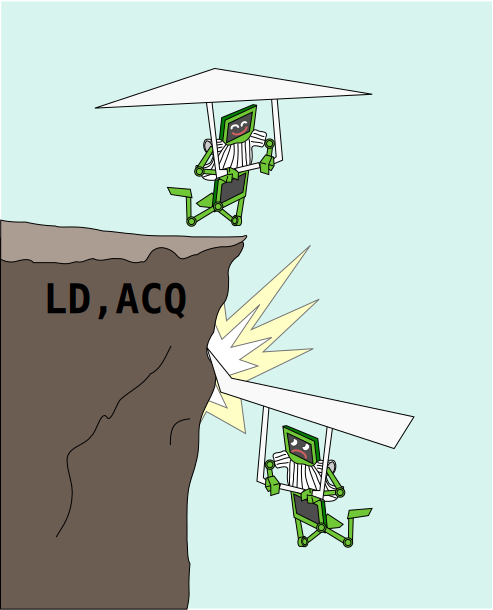
\includegraphics{cartoons/r-2014-LD-ACQ}}
\end{center}
\caption{Half Memory Barrier}
\ContributedBy{Figure}{fig:app:whymb:Half Memory Barrier}{Melissa Brossard}
\end{figure}

이 half-memory fence 들은 오퍼레이션들을 크리티컬 섹션에 안전하게 집어넣을 수
있으므로 크리티컬 섹션에 유용합니다만, 이 오퍼레이션들이 삐져나오게 되면 매우
위험합니다.
IA64 는 이 기능을 제공하는 CPU 들 중 하나\footnote{
	ARMv8 은 최근 load-acquire 와 store-release 인스트럭션들을
	추가했습니다.}
로써 리눅스의 락 획득과 해제에 연관된 메모리 오퍼레이션 순서 의미를 정의합니다.
크리티컬 섹션은 오퍼레이션들을 집어넣기 안전하지만 바깥으로 삐져나오면
치명적이기에 이 half-memory fence 들은 크리티컬 섹션에 유용합니다.
\iffalse

These half-memory fences are useful for critical sections, since
it is safe to push operations into a critical section, but can be
fatal to allow them to bleed out.
However, as one of the only CPUs with this property,\footnote{
	ARMv8 has recently added load-acquire and store-release instructions.}
IA64 defines
Linux's semantics of memory ordering associated with lock acquisition
and release.
\fi

IA64 {\tt mf} 인스트럭션이 리눅스 커널의 {\tt smp\_rmb()}, {\tt smp\_mb()},
그리고 {\tt smp\_wmb()} 기능을 위해 사용됩니다.
아, 그리고 모순되는 루머들이 있긴 하지만, ``mf'' 는 정말로 ``memory fence'' 의
약자입니다.

마지막으로, IA64 는 ``release'' 오퍼레이션과 ``mf'' 인스트럭션들에 글로벌한
전체 순서를 제공합니다.
이는 한 코드 조각이 한 액세스가 일어난 것으로 본다면, 그 뒤의 코드 조각들도
역시 그 앞의 액세스가 일어난 것으로 보게 되는 타동성의 개념을 제공합니다.
이는 모든 코드 조각들이 올바르게 메모리 배리어들을 사용했다는 가정 하의
이야기입니다.
\iffalse

The IA64 {\tt mf} instruction is used for the {\tt smp\_rmb()},
{\tt smp\_mb()}, and {\tt smp\_wmb()} primitives in the Linux kernel.
Oh, and despite rumors to the contrary, the ``mf'' mnemonic really
does stand for ``memory fence''.

Finally, IA64 offers a global total order for ``release'' operations,
including the ``mf'' instruction.
This provides the notion of transitivity, where if a given code fragment
sees a given access as having happened, any later code fragment will
also see that earlier access as having happened.
Assuming, that is, that all the code fragments involved correctly use
memory barriers.
\fi

\subsection{MIPS}

MIPS 메모리 모델~\cite[Table 6.6]{MIPSvII-A-2015} 은 ARM, IA64, 그리고 Power 와
흡사해서 완화된 순서를 기본으로 합니다만 의존성을 지켜줍니다.
MPIS 는 다양한 종류의 메모리 배리어 인스트럭션들을 갖습니다만,  ARM64 추가
인스트럭션들처럼 하드웨어 관점이 아니라 리눅스 커널과 C++11
표준~\cite{RichardSmith2015N4527} 에서 제공되는 사용예 관점으로 분류되어
있습니다:
\iffalse

The MIPS memory model~\cite[Table 6.6]{MIPSvII-A-2015}
appears to resemble that of ARM, IA64, and Power,
being weakly ordered by default, but respecting dependencies.
MIPS has a wide variety of memory-barrier instructions, but ties them
not to hardware considerations, but rather to the use cases provided
by the Linux kernel and the C++11 standard~\cite{RichardSmith2015N4527}
in a manner similar to the ARM64 additions:
\fi

\begin{description}
\item[SYNC]
	메모리 참조 외에도 여러 하드웨어 오퍼레이션들을 위한 전체 배리어
	\iffalse

	Full barrier for a number of hardware operations in addition
	to memory references.
	\fi
\item[SYNC\_WMB]
	리눅스 커널의 \co{smp_wbm()} 구현을 위해 사용될 수 있는 쓰기 메모리
	배리어.
	\iffalse

	Write memory barrier, which can be used to implement the
	\co{smp_wmb()} primitive in the Linux kernel.
	\fi
\item[SYNC\_MB]
	메모리 오퍼레이션들에만 적용되는 전체 메모리 배리어.
	이 기능은 리눅스 커널의 \co{smp_mb()} 와 C++
	\co{atomic_thread_fence(memory_order_seq_cst)} 의 구현에 사용될 수
	있습니다.
	\iffalse

	Full memory barrier, but only for memory operations.
	This may be used to implement the Linux-kernel \co{smp_mb()}
	and the C++ \co{atomic_thread_fence(memory_order_seq_cst)}.
	\fi
\item[SYNC\_ACQUIRE]
	리눅스 커널의 \co{smp_load_acquire()} 와 C++
	\co{atomic_load_explicit(..., memory_order_acquire)} 구현에 사용될 수
	있는 Acquire 메모리 배리어.
	\iffalse

	Acquire memory barrier, which may be used to implement the
	Linux-kernel \co{smp_load_acquire()} and the C++
	\co{atomic_load_explicit(..., memory_order_acquire)}.
	\fi
\item[SYNC\_RELEASE]
	리눅스 커널의 \co{smp_store_release()} 와 C++
	\co{atomic_store_explicit(..., memory_order_release)} 의 구현에 사용될
	수 있는 Release 메모리 배리어.
	\iffalse

	Release memory barrier, which may be used to implement the
	Linux-kernel \co{smp_store_release()} and the C++
	\co{atomic_store_explicit(..., memory_order_release)}.
	\fi
\item[SYNC\_RMB]
	리눅스 커널의 \co{smp_rmb()} 구현에 사용될 수 있는 읽기 메모리 배리어.
	\iffalse

	Read memory barrier, which can be used to implement the
	\co{smp_rmb()} primitive in the Linux kernel.
	\fi
\end{description}

MIPS 아키텍쳐에 대한 비공식적 토의들은 MIPS 가 ARM 과 Power 의 그것과 유사한
타동성과 누적성을 가짐을 알려줍니다.
하지만, 다른 MIPS 구현은 다른 메모리 순서 특성을 가질 수 있으므로, 당신이
사용하고 있는 특정 MIPS 구현을 위해서는 문서를 참고하는게 좋습니다.
\iffalse

Informal discussions with MIPS architects indicates that MIPS has a
definition of transitivity or cumulativity similar to that of
ARM and Power.
However, it appears that different MIPS implementations can have
different memory-ordering properties, so it is important to consult
the documentation for the specific MIPS implementation you are using.
\fi

\subsection{PA-RISC}

PA-RISC 아키텍쳐는 로드와 스토어의 완전한 재배치를 허용하지만, 실제 CPU 들은
순서를 지킵켜니다~\cite{GerryKane96a}.
이는 리눅스 커널의 메모리 순서 기능들이 어떤 코드도 만들어내지 않을 것임을
의미합니다만, 실제로는 메모리 배리어 전후로 코드를 재배치 할 수 있는 컴파일러
최적화를 막기 위해 gcc 의 {\tt memory} 한정사를 사용합니다.
\iffalse

Although the PA-RISC architecture permits full reordering of loads and
stores, actual CPUs run fully ordered~\cite{GerryKane96a}.
This means that the Linux kernel's memory-ordering primitives generate
no code, however, they do use the gcc {\tt memory} attribute to disable
compiler optimizations that would reorder code across the memory
barrier.
\fi

\subsection{POWER / PowerPC}
\label{sec:app:whymb:POWER / PowerPC}

POWER 와 PowerPC\textsuperscript{\textregistered} CPU 계열은 다양한 메모리
배리어 인스트럭션들을 가지고 있습니다~\cite{PowerPC94,MichaelLyons02a}:
\begin{enumerate}
\item	{\tt sync} 는 모든 앞의 오퍼레이션들이 뒤의 오퍼레이션이 하나라도
	시작하기 전에 완료된 {\em 것처럼 보이게} 합니다.
	따라서 이 인스트럭션은 상당히 비용이 비쌉니다.
\item	{\tt lwsync} (light-weight sync) 는 로드 오퍼레이션들을 뒤의 로드와
	스토어 오퍼레이션들에 대해 순서 맞추며, 스토어 오퍼레이션 역시 순서를
	맞춰줍니다.
	하지만, 스토어 오퍼레이션들을 뒤의 로드들에 대해 순서맞추지는 {\em
	않습니다}.
	흥미롭게도, {\tt lwsync} 인스트럭션은 zSeries, 그리고 우연히도, SPARC
	TSO 와 같은 순서 규칙을 강제합니다.
	\co{lwsync} 인스트럭션은 load-acquire 와 store-release 오퍼레이션을
	구현하는데 사용될 수도 있습니다.
\item	{\tt eieio} (enforce in-order execution of I/O, in case you were
	wondering) 은 앞의 모든 캐싱 기능한 스토어들을 뒤의 스토어들 이전에
	완료된 것으로 나타나게 합니다.
	하지만, 캐싱 가능한 메모리로의 스토어들은 캐싱 불가능한 메모리로의
	스토어들과는 별개로 순서지어지는데, 이는 {\tt eieio} 가 MMIO 스토어가
	스핀락 해제 뒤로 재배치 되는 현상도 막지 않는다는 뜻입니다.
\item	{\tt isync} 는 뒤의 인스트럭션이 하나라도 실행을 시작하기 이전에 앞의
	인스트럭션들이 완료된 것으로 나타나게 만듭니다.
	이는 앞의 인스트럭션들은 그들이 만들 수 있는 어떤 트랩도 이미
	일어났거나 일어나지 않도록 보장될 만큼 충분히 진행되었어야 하며, 이
	인스트럭션들의 어떤 사이드 이펙트들 (예를 들어, 페이지 테이블의 변경)
	도 뒤의 인스트럭션들에게 보여야 함을 의미합니다.
\end{enumerate}
\iffalse

The POWER and PowerPC\textsuperscript{\textregistered}
CPU families have a wide variety of memory-barrier
instructions~\cite{PowerPC94,MichaelLyons02a}:
\begin{enumerate}
\item	{\tt sync} causes all preceding operations to {\em appear to have}
	completed before any subsequent operations are started.
	This instruction is therefore quite expensive.
\item	{\tt lwsync} (light-weight sync) orders loads with respect to
	subsequent loads and stores, and also orders stores.
	However, it does {\em not} order stores with respect to subsequent
	loads.
	Interestingly enough, the {\tt lwsync} instruction enforces
	the same ordering as does zSeries, and coincidentally,
	SPARC TSO.
	The \co{lwsync} instruction may be used to implement
	load-acquire and store-release operations.
\item	{\tt eieio} (enforce in-order execution of I/O, in case you
	were wondering) causes all preceding cacheable stores to appear
	to have completed before all subsequent stores.
	However, stores to cacheable memory are ordered separately from
	stores to non-cacheable memory, which means that {\tt eieio}
	will not force an MMIO store to precede a spinlock release.
\item	{\tt isync} forces all preceding instructions to appear to have
	completed before any subsequent instructions start execution.
	This means that the preceding instructions must have progressed
	far enough that any traps they might generate have either happened
	or are guaranteed not to happen, and that any side-effects of
	these instructions (for example, page-table changes) are seen by the
	subsequent instructions.
\end{enumerate}
\fi

불행히도, 이 인스트럭션들 중 어떤 것도 {\em 모든} 스토어들을 순서 맞추지만 {\tt
sync} 인스트럭션처럼 큰 오버헤드의 많은 동작을 요하지는 않는, 리눅스의 {\tt
wbm()} 기능과 일치하지 않습니다.
하지만 선택의 여지가 없습니다: {\tt wmb()} 와 {\tt mb()} 의 ppc64 버전은 좀
무겁지만 {\tt sync} 인스트럭션을 사용하게 되어 있습니다.
하지만, 리눅스의 {\tt smp\_wmb()} 인스트럭션은 (어차피 드라이버가 MMIO 의
순서를 UP 커널 에서도 SMP 커널에서도 알아서 순서를 맞춰야 하므로) MMIO 에
사용하지 않기 때문에, 가벼운 {\tt eieio} 인스트럭션으로 구현되어 있습니다.
이 인스트럭션은 다섯개 모음의 약자라 좀 독특해 보일 수 있습니다.
{\tt smp\_mb()} 인스트럭션 또한 {\tt sync} 인스트럭션으로 정의되어 있습니다만,
{\tt smp\_rmb()} 와 {\tt rmb()} 는 가벼운 {\tt lwsync} 인스트럭션으로 정의되어
있습니다.
\iffalse

Unfortunately, none of these instructions line up exactly with Linux's
{\tt wmb()} primitive, which requires {\em all} stores to be ordered,
but does not require the other high-overhead actions of the {\tt sync}
instruction.
But there is no choice: ppc64 versions of {\tt wmb()} and {\tt mb()} are
defined to be the heavyweight {\tt sync} instruction.
However, Linux's {\tt smp\_wmb()} instruction is never used for MMIO
(since a driver must carefully order MMIOs in UP as well as
SMP kernels, after all), so it is defined to be the lighter weight
{\tt eieio} instruction.
This instruction may well be unique in having a five-vowel mnemonic.
The {\tt smp\_mb()} instruction is also defined to be the {\tt sync}
instruction, but both {\tt smp\_rmb()} and {\tt rmb()} are defined to
be the lighter-weight {\tt lwsync} instruction.
\fi

Power 는 타동성을 얻기 위해 사용될 수 있는, ``누적성'' 을 가지고 있습니다.
제대로 사용된다면, 앞의 코드 조각의 결과를 보는 코드는 이 앞의 코드 조각이 봤던
결과 역시 볼 수 있을 것입니다.
더 자세한 건 McKenney 와 Silvera의 작업물~\cite{PaulEMcKenneyN2745r2009} 에서
볼 수 있습니다.

Power \co{isync} 인스트럭션이 ARM \co{ISB} 인스트럭션으로 대체된다는 점을
제외하고는, Power 는 ARM 에서 하는 것과 같은 방식으로 컨트롤 의존성을
지켜줍니다.
\iffalse

Power features ``cumulativity'', which can be used to obtain
transitivity.
When used properly, any code seeing the results of an earlier
code fragment will also see the accesses that this earlier code
fragment itself saw.
Much more detail is available from
McKenney and Silvera~\cite{PaulEMcKenneyN2745r2009}.

Power respects control dependencies in much the same way that ARM
does, with the exception that the Power \co{isync} instruction
is substituted for the ARM \co{ISB} instruction.
\fi

POWER 아키텍쳐의 많은 멤버들이 일관성을 지키지 않는 인스트럭션 캐시를 가지고
있어서, 인스트럭션이 위치하는 메모리로의 스토어는 인스트럭션 캐시에 제대로
반영되지 않을 수 있습니다.
감사하게도, 오늘날에는 적은 사람들만이 스스로를 수정하는 코드를 작성합니다만,
JIT 들과 컴파일러들은 항상 그 짓을 합니다.
더욱이, 최근에 수행된 프로그램을 다시 컴파일 하는 행위는 CPU 의 관점에서는
스스로를 수정하는 코드처럼 보입니다.
{\tt icbl} (instruction cache block invalidate) 인스트럭션은 인스트럭션
캐시에서 특정 캐시 라인을 무효화 하게 하므로, 이런 상황에 사용될 수 있을
것입니다.
\iffalse

Many members of the POWER architecture have incoherent instruction
caches, so that a store to memory will not necessarily be reflected
in the instruction cache.
Thankfully, few people write self-modifying code these days, but JITs
and compilers do it all the time.
Furthermore, recompiling a recently run program looks just like
self-modifying code from the CPU's viewpoint.
The {\tt icbi} instruction (instruction cache block invalidate)
invalidates a specified cache line from
the instruction cache, and may be used in these situations.
\fi

\subsection{SPARC RMO, PSO, and TSO}

Solaris on SPARC uses TSO (total-store order), as does Linux when built for
the ``sparc'' 32-bit architecture.
However, a 64-bit Linux kernel (the ``sparc64'' architecture)
runs SPARC in RMO (relaxed-memory order) mode~\cite{SPARC94}.
The SPARC architecture also offers an intermediate PSO (partial store
order).
Any program that runs in RMO will also run in either PSO or TSO, and similarly,
a program that runs in PSO will also run in TSO.
Moving a shared-memory parallel program in the other direction may
require careful insertion of memory barriers, although, as noted earlier,
programs that make standard use of synchronization primitives need not
worry about memory barriers.

SPARC has a very flexible memory-barrier instruction~\cite{SPARC94}
that permits fine-grained control of ordering:
\begin{itemize}
\item	{\tt StoreStore}: order preceding stores before subsequent stores.
	(This option is used by the Linux {\tt smp\_wmb()} primitive.)
\item	{\tt LoadStore}: order preceding loads before subsequent stores.
\item	{\tt StoreLoad}: order preceding stores before subsequent loads.
\item	{\tt LoadLoad}: order preceding loads before subsequent loads.
	(This option is used by the Linux {\tt smp\_rmb()} primitive.)
\item	{\tt Sync}: fully complete all preceding operations before starting
	any subsequent operations.
\item	{\tt MemIssue}: complete preceding memory operations before subsequent
	memory operations, important for some instances of memory-mapped
	I/O.
\item	{\tt Lookaside}: same as MemIssue, but only applies to preceding stores
	and subsequent loads, and even then only for stores and loads that
	access the same memory location.
\end{itemize}

The Linux {\tt smp\_mb()} primitive uses the first four options together,
as in
{\tt membar \#LoadLoad | \#LoadStore | \#StoreStore | \#StoreLoad},
thus fully ordering memory operations.

So, why is {\tt membar \#MemIssue} needed?
Because a {\tt membar \#StoreLoad} could permit a subsequent
load to get its value from a write buffer, which would be
disastrous if the write was to an MMIO register that induced side effects
on the value to be read.
In contrast, {\tt membar \#MemIssue} would wait until the write buffers
were flushed before permitting the loads to execute,
thereby ensuring that the load actually gets its value from the MMIO register.
Drivers could instead use {\tt membar \#Sync}, but the lighter-weight
{\tt membar \#MemIssue} is preferred in cases where the additional function
of the more-expensive {\tt membar \#Sync} are not required.

The {\tt membar \#Lookaside} is a lighter-weight version of
{\tt membar \#MemIssue}, which is useful when writing to a given MMIO register
affects the value that will next be read from that register.
However, the heavier-weight {\tt membar \#MemIssue} must be used when
a write to a given MMIO register affects the value that will next be
read from {\em some other} MMIO register.

It is not clear why SPARC does not define {\tt wmb()} to be
{\tt membar \#MemIssue} and {\tt smb\_wmb()} to be
{\tt membar \#StoreStore},
as the current definitions seem vulnerable to bugs in some drivers.
It is quite possible that all the SPARC CPUs that Linux runs on
implement a more conservative memory-ordering model than the architecture
would permit.

SPARC requires a {\tt flush} instruction be used between the time that
an instruction is stored and executed~\cite{SPARC94}.
This is needed to flush any prior value for that location from
the SPARC's instruction cache.
Note that {\tt flush} takes an address, and will flush only that address
from the instruction cache.
On SMP systems, all CPUs' caches are flushed, but there is no
convenient way to determine when the off-CPU flushes complete,
though there is a reference to an implementation note.

\subsection{x86}

Since the x86 CPUs provide ``process ordering'' so that all CPUs agree
on the order of a given CPU's writes to memory, the {\tt smp\_wmb()} primitive
is a no-op for the CPU~\cite{IntelXeonV3-96a}.
However, a compiler directive is required to
prevent the compiler from performing optimizations that would result
in reordering across the {\tt smp\_wmb()} primitive.

On the other hand, x86 CPUs have traditionally given
no ordering guarantees for loads, so
the {\tt smp\_mb()} and {\tt smp\_rmb()} primitives expand to {\tt lock;addl}.
This atomic instruction acts as a barrier to both loads and stores.

Intel has also published a memory model for
x86~\cite{Intelx86MemoryOrdering2007}.
It turns out that Intel's actual CPUs enforced tighter ordering than
was claimed in the previous specifications, so this model is in effect
simply mandating the earlier de-facto behavior.
Even more recently, Intel published an updated memory model for
x86~\cite[Section 8.2]{Intel64IA32v3A2011}, which mandates a total global order
for stores, although individual CPUs are still permitted to see their
own stores as having happened earlier than this total global order
would indicate.
This exception to the total ordering is needed to allow important
hardware optimizations involving store buffers.
In addition, memory ordering obeys causality, so that if CPU~0 sees a
store by CPU~1, then CPU~0 is guaranteed to see all stores that CPU~1
saw prior to its store.
Software may use atomic operations to override these hardware optimizations,
which is one reason that atomic operations tend to be more expensive
than their non-atomic counterparts.
This total store order is \emph{not} guaranteed on older processors.

It is also important to note that atomic instructions operating
on a given memory location should all be of the same
size~\cite[Section 8.1.2.2]{Intel64IA32v3A2011}.
For example, if you write a program where one CPU atomically increments
a byte while another CPU executes a 4-byte atomic increment on
that same location, you are on your own.

However, note that some SSE instructions are weakly ordered ({\tt clflush}
and non-temporal move instructions~\cite{IntelXeonV2b-96a}).
CPUs that have SSE can use {\tt mfence} for {\tt smp\_mb()},
{\tt lfence} for {\tt smp\_rmb()}, and {\tt sfence} for {\tt smp\_wmb()}.

A few versions of the x86 CPU have a mode bit that enables out-of-order
stores, and for these CPUs, {\tt smp\_wmb()} must also be defined to
be {\tt lock;addl}.

Although newer x86 implementations accommodate self-modifying code
without any special instructions, to be fully compatible with
past and potential future x86 implementations, a given CPU must
execute a jump instruction or a serializing instruction (e.g., \co{cpuid})
between modifying the code and executing
it~\cite[Section 8.1.3]{Intel64IA32v3A2011}.

\subsection{zSeries}

The zSeries machines make up the IBM\textsuperscript{\texttrademark}
mainframe family, previously
known as the 360, 370, and 390~\cite{IBMzSeries04a}.
Parallelism came late to zSeries, but given that these mainframes first
shipped in the mid 1960s, this is not saying much.
The {\tt bcr 15,0} instruction is used for the Linux {\tt smp\_mb()},
{\tt smp\_rmb()}, and {\tt smp\_wmb()} primitives.
It also has comparatively strong memory-ordering semantics, as shown in
Table~\ref{tab:app:whymb:Summary of Memory Ordering}, which should allow the
{\tt smp\_wmb()} primitive to be a {\tt nop} (and by the time you read this,
this change may well have happened).
The table actually understates the situation, as the zSeries memory model
is otherwise sequentially consistent, meaning that all CPUs
will agree on the order of unrelated stores from different CPUs.

As with most CPUs, the zSeries architecture does not guarantee a
cache-coherent instruction stream, hence,
self-modifying code must execute a serializing instruction between updating
the instructions and executing them.
That said, many actual zSeries machines do in fact accommodate self-modifying
code without serializing instructions.
The zSeries instruction set provides a large set of serializing instructions,
including compare-and-swap, some types of branches (for example, the
aforementioned {\tt bcr 15,0} instruction), and test-and-set,
among others.

\section{Are Memory Barriers Forever?}
\label{sec:app:whymb:Are Memory Barriers Forever?}

There have been a number of recent systems that are significantly less
aggressive about out-of-order execution in general and re-ordering
memory references in particular.
Will this trend continue to the point where memory barriers are a thing
of the past?

The argument in favor would cite proposed massively multi-threaded hardware
architectures, so that each thread would wait until memory was ready,
with tens, hundreds, or even thousands of other threads making progress
in the meantime.
In such an architecture, there would be no need for memory barriers,
because a given thread would simply wait for all outstanding operations
to complete before proceeding to the next instruction.
Because there would be potentially thousands of other threads, the
CPU would be completely utilized, so no CPU time would be wasted.

The argument against would cite the extremely limited number of applications
capable of scaling up to a thousand threads, as well as increasingly
severe realtime requirements, which are in the tens of microseconds
for some applications.
The realtime-response requirements are difficult enough to meet as is,
and would be even more difficult to meet given the extremely low
single-threaded throughput implied by the massive multi-threaded
scenarios.

Another argument in favor would cite increasingly sophisticated
latency-hiding hardware implementation techniques that might well allow
the CPU to provide the illusion of fully sequentially consistent
execution while still providing almost all of the performance advantages
of out-of-order execution.
A counter-argument would cite the increasingly severe power-efficiency
requirements presented both by battery-operated devices and by
environmental responsibility.

Who is right?
We have no clue, so are preparing to live with either scenario.

\section{Advice to Hardware Designers}
\label{sec:app:whymb:Advice to Hardware Designers}

There are any number of things that hardware designers can do
to make the lives of software people difficult.
Here is a list of a few such things that we have encountered in
the past, presented here in the hope that it might help prevent
future such problems:
\begin{enumerate}
\item	I/O devices that ignore cache coherence.

	This charming misfeature can result in DMAs from memory
	missing recent changes to the output buffer, or, just as
	bad, cause input buffers to be overwritten by the contents
	of CPU caches just after the DMA completes.
	To make your system work in face of such misbehavior,
	you must carefully flush the CPU caches of any location
	in any DMA buffer before presenting that buffer to the
	I/O device.
	Similarly, you need to flush the CPU caches of any location
	in any DMA buffer after DMA to that buffer completes.
	And even then, you need to be \emph{very} careful to avoid
	pointer bugs, as even a misplaced read to an input buffer
	can result in corrupting the data input!

\item	External busses that fail to transmit cache-coherence data.

	This is an even more painful variant of the above problem,
	but causes groups of devices---and even memory itself---to
	fail to respect cache coherence.
	It is my painful duty to inform you that as embedded systems
	move to multicore architectures, we will no doubt see a fair
	number of such problems arise.
	Hopefully these problems will clear up by the year 2015.

\item	Device interrupts that ignore cache coherence.

	This might sound innocent enough --- after all, interrupts
	aren't memory references, are they?
	But imagine a CPU with a split cache, one bank of which is
	extremely busy, therefore holding onto the last cacheline
	of the input buffer.
	If the corresponding I/O-complete interrupt reaches this
	CPU, then that CPU's memory reference to the last cache
	line of the buffer could return old data, again resulting
	in data corruption, but in a form that will be invisible
	in a later crash dump.
	By the time the system gets around to dumping the offending
	input buffer, the DMA will most likely have completed.

\item	Inter-processor interrupts (IPIs) that ignore cache coherence.

	This can be problematic if the IPI reaches its destination
	before all of the cache lines in the corresponding message
	buffer have been committed to memory.

\item	Context switches that get ahead of cache coherence.

	If memory accesses can complete too wildly out of order,
	then context switches can be quite harrowing.
	If the task flits from one CPU to another before all the
	memory accesses visible to the source CPU make it to the
	destination CPU, then the task could easily see the corresponding
	variables revert to prior values, which can fatally confuse
	most algorithms.

\item	Overly kind simulators and emulators.

	It is difficult to write simulators or emulators that force
	memory re-ordering, so software that runs just fine in
	these environments can get a nasty surprise when it first
	runs on the real hardware.
	Unfortunately, it is still the rule that the hardware is more
	devious than are the simulators and emulators, but we hope that
	this situation changes.
\end{enumerate}

Again, we encourage hardware designers to avoid these practices!
